% 150 câu đã gỡ khỏi ngân hàng (chuyen_dang) — chép lại vào file dạng để khôi phục

% từ: cau-hoi/lop10/0D0_Xac_suat/0D0-1-3_Dem_phan_tu_khong_gian_mau_bien_co.tex
\begin{bt}%[0D0V1-3]%[ma:5587eb25]
	Cho tập $Q = \left\{1; 2; 3; 4; 5; 6\right\}$. Từ tập $Q$ có thể lập được bao nhiêu số tự nhiên có $3$ chữ số khác nhau. Tính số phần tử  của biến cố sao cho số được chọn nhỏ hơn $345$.
	\shortans{50} 
	\loigiai{ 
		Gọi  $A$ là biến cố: \lq\lq Số được chọn nhỏ hơn $345$\rq\rq.\\
		Số  tự nhiên có ba chữ số thuộc $A$ là $\overline{abc}$, với $a$, $b$, $c$ thuộc $Q = \left\{1; 2; 3; 4; 5; 6\right\}$ và đôi một khác nhau.
		\begin{itemize}
			 \item Trường hợp $a = 3$.\\
			 $+$ Nếu $b = 4$ thì $c \in \{1; 2\}$. Có $2$ số tự nhiên thỏa mãn.\\
			$+$ Nếu $b \in \{1; 2\}$ thì  $b$ có $2$ cách chọn và $c$ có $4$ cách chọn. Có $2 \cdot 4 = 8$ số tự nhiên thỏa mãn.\\
			Trường hợp  này có $2 + 8 = 10$ số thỏa mãn.
			\item Trường hợp $a \in \{1;  2\}$.\\
			Khi đó $a$ có $2$ cách chọn, $b$ có $5$  cách chọn và $c$ có $4$ cách chọn. Vậy có $2\cdot 5\cdot 4 = 40$ số tự nhiên thỏa mãn.
		\end{itemize}
		Theo quy tắc cộng ta có $ 10 + 40 = 50$ số  tự nhiên thỏa mãn.
		Do  đó $n\left(A\right) = 50$.
	} 
\end{bt}

% từ: cau-hoi/lop10/0D1_Menh_de_Tap_hop/0D1-1-4_Menh_de_keo_theo_menh_de_dao_menh_de_tuong_du.tex
\begin{bt}%[0D1H1-4]%[ma:7d466243]
	Cho tam giác $ABC$. Xét hai mệnh đề $P\colon $ ``tam giác $ABC$ vuông'' và $Q\colon$ ``$AB^2+AC^2=BC^2$''. Phát biểu và cho biết mệnh đề sau đúng hay sai.
	\begin{listEX}[2]
		\item $P \Rightarrow Q$.
		\item $Q \Rightarrow P$.
	\end{listEX}
	\loigiai{
		\begin{listEX}
			\item Mệnh đề $P \Rightarrow Q$ là ``Nếu tam giác $ABC$ vuông thì $AB^2+AC^2=BC^2$''.\\
			Mênh đề $P \Rightarrow Q$ sai vì chưa chắc tam giác đã vuông tại $A$.
			\item Mệnh đề $Q \Rightarrow P$ là ``Nếu tam giác $ABC$ có $AB^2+AC^2=BC^2$ thì tam giác vuông''.\\
			Mệnh đề $Q \Rightarrow P$ đúng (theo định lí Pitago).
		\end{listEX}
	}
\end{bt}

% từ: cau-hoi/lop10/0D1_Menh_de_Tap_hop/0D1-2-1_Tap_hop_va_phan_tu_cua_tap_hop.tex
\begin{ex}%[0D1N2-1]%[ma:fc41e07f]
	Ký hiệu nào sau  đây đúng với định nghĩa \lq\lq$3$ là một số tự nhiên\rq\rq?
	 \choice
		{$3  \subset \mathbb{N}$}
		{\True $3  \in \mathbb{N}$}
		{$3 \not\in  \mathbb{N}$}
		{$3 \leq  \mathbb{N}$}
	\loigiai{ 
		Đáp án $3 \subset \mathbb{N}$ sai vì ký hiệu \lq\lq$\subset$\rq\rq\, chỉ dùng cho hai tập hợp mà không dùng  cho \lq\lq$3$\rq\rq\, là một số.\\
		Hai đáp án $3 \not\in \mathbb{N}$ và $3 \leq \mathbb{N}$ đều  sai vì ta không muốn so sánh số với tập hợp.
	 }
\end{ex}

% từ: cau-hoi/lop10/0D1_Menh_de_Tap_hop/0D1-2-1_Tap_hop_va_phan_tu_cua_tap_hop.tex
\begin{bt}%[0D1N2-1]%[ma:39da5f17]
	Biểu diễn các tập hợp sau bằng biểu đồ Ven.
	\begin{multicols}{2}
	\begin{enumerate}
		\item $A=\{0; 1; 2; 3\}$;
		\item $B=\{\text{Lan}; \text{Huệ}; \text{Trang} \}$		
	\end{enumerate}
	\end{multicols}
	\loigiai{
		\begin{enumerate}
			\item Biểu đồ Ven biểu diễn tập hợp $\mathrm{A}=\{0;1;2;3\}$ là 
			\begin{center}
				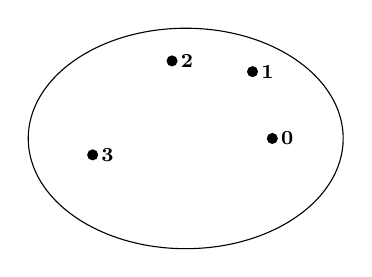
\begin{tikzpicture}[>=stealth,line join=round,line cap=round,font=\footnotesize,scale=1]
					\draw (0,0) ellipse (2 and 1.4);
					\foreach \goc/\ra/\lb in {0/1.1/0,45/1.2/1,100/1/2,190/1.2/3}{
						\fill (0,0)+(\goc:\ra)circle(2pt)node[right]{$\mathbf{\lb}$};
					}				
				\end{tikzpicture}
			\end{center}
			\item Biểu đồ Ven biểu diễn tập hợp $\mathrm{A}=\{\text{Lan};\text{Huệ};\text{Trang}\}$ là 
			\begin{center}
				\begin{tikzpicture}[>=stealth,line join=round,line cap=round,font=\footnotesize,scale=1]
					\draw (0,0) ellipse (2 and 1.4);
					\foreach \goc/\ra/\lb in {0/1.1/Lan,100/1.2/Huệ,180/1/Trang}{
						\fill (0,0)+(\goc:\ra)circle(2pt)node[below]{\lb};
					}				
				\end{tikzpicture}
			\end{center}		
		\end{enumerate}
	}
\end{bt}

% từ: cau-hoi/lop10/0D1_Menh_de_Tap_hop/0D1-2-3_Ky_hieu_khoang_doan_nua_khoang.tex
\begin{bt}%[0D1Y2-3]%[0D1B3-1]%[ma:1eb8dd1b]
	Cho hai  tập hợp $A=[1;4]$ và $B=(3;6)$.
	\begin{enumerate}
		\item Biểu  diễn tập $A$ và tập $B$ trên từng trục số.
		 \item Xác định các tập hợp $A\cup B$, $A\cap B$.
	\end{enumerate}
	 \loigiai{
		\begin{enumerate}
			\item Tập hợp $A$ 
			\begin{center}
				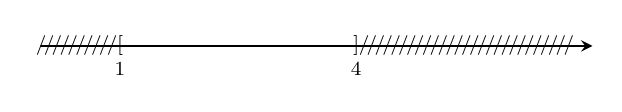
\begin{tikzpicture}[font=\footnotesize,line cap=round,line join=round,thick]
						\node  at (1,0) {$[$};
						 \node at (4,0) {$]$};
						\draw[-stealth]  (0,0)--(1,0) node[below=3pt]{$1$}--(4,0) node[below=3pt]{$4$}--(7,0);
						\foreach \x in {0,.1,.2,...,.9} 
						\draw (\x,0)  node{$/$};
						 \foreach \y in {4.1,4.2,...,6.7}
						\draw (\y,0)  node{$/$};
					\end{tikzpicture}
			\end{center}
			Tập hợp $B$ 
			\begin{center}
				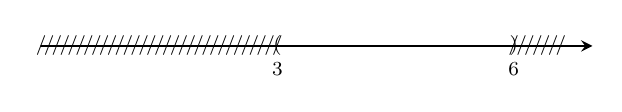
\begin{tikzpicture}[font=\footnotesize,line cap=round,line join=round,thick]
						\node  at (3,0) {$($};
						\node at  (6,0) {$)$};
						\draw[-stealth]  (0,0)--(3,0) node[below=3pt]{$3$}--(6,0) node[below=3pt]{$6$}--(7,0);
						\foreach \x  in {0,.1,.2,...,3}
						\draw  (\x,0) node{$/$};
						 \foreach \y in {6,6.1,...,6.7}
						 \draw (\y,0) node{$/$};
					\end{tikzpicture}
			\end{center}
			\item $A\cup  B = [1;6)$, $A\cap B= (3;4]$.
		\end{enumerate}
	} 
\end{bt}

% từ: cau-hoi/lop10/0D1_Menh_de_Tap_hop/0D1-3-1_Giao_va_hop_cua_hai_tap_hop_roi_rac.tex
\begin{ex}%[0D1K3-1]%[ma:848e9758]
	Cho hai tập hợp $A=\left\{x\in \mathbb{R}\big|\left(x^2-1 \right)\left(x^2-3x+4  \right)=0 \right\}$ và $B=\left\{x\in \mathbb{Z}\big|\left| x \right|\leq 2 \right\}$. Tìm tập hợp $A\cup B$.
	\choice 
		 {\True $\left\{-2,-1,0,1,2 \right\}$}
		{$\left\{-2,-1,0,1,2, -4  \right\}$}
		{$\left\{-1, 1  \right\}$}
		{$\left\{-2, 0,  2\right\}$}
	 \loigiai{
		Ta có $A=\left\{-1, 1\right\}, B=\left\{-2, -1, 0, 1,  2\right\}$. Suy ra $A\cup B =\left\{-2, -1, 0, 1, 2\right\}$.
	} 
\end{ex}

% từ: cau-hoi/lop10/0D2_BPT_va_he_BPT_bac_nhat_hai_an/0D2-1-2_Mien_nghiem_cua_BPT_bac_nhat_hai_an.tex
\begin{ex}%[0D2H1-2]%[ma:68e1172e]
	Đường thẳng $d\colon 2x-y=2$ chia mặt phẳng tọa độ thành hai miền I, II có bờ là đường thẳng $d$. Xác định miền nghiệm của bất phương  trình $2x-y\ge 2$.
	\begin{center}
		\begin{tikzpicture}[line join=round,line cap=round,>=stealth]
				\tikzset{every  node/.style={scale=0.9}}
				\draw[->] (-1.1,0)--(3.1,0) node[below left]  {$x$};
				 \draw[->] (0,-2.5)--(0,3.1) node[below left] {$y$};
				\draw (0,0)  node [below left] {$O$};
				 \foreach \x/\nx in {1/1,2/2}
				\draw[thin]  (\x,1pt)--(\x,-1pt) node [below] {$\nx$};
				 \foreach \y/\ny in {-2/-2,-1/-1,1/1,2/2}
				\draw[thin] (1pt,\y)--(-1pt,\y) node [left] {$\ny$}; 
				\begin{scope}
					\clip (-1,-2.5)  rectangle (3,3);
					 \draw[samples=200,domain=-1:3,smooth,variable=\x] plot (\x,{2*(\x)+-2});
				\end{scope}
				 \node [right,rotate=65] at (1,.5){$2x-y=2$};
				\path (0.5,1.5) node [above]{II}; 
				\path (2,0.5)  node [above]{I};
			\end{tikzpicture}
	\end{center}
	 \choice
		{Nửa  mặt phẳng I không kể đường thẳng $d$}
		{\True Nửa mặt phẳng I kể cả đường  thẳng $d$}
		{Nửa  mặt phẳng II kể cả đường thẳng $d$}
		{Nửa mặt phẳng II  không kể đường thẳng $d$}
	 \loigiai{
		Thay tọa độ điểm $O(0;0)$ vào bất phương trình đã cho $2x-y\ge 2$, ta có $2\cdot0 -0\ge 2$ là mệnh đề sai. Do vậy  miền nghiệm của bất phương trình đã cho là miền I không chứa điểm $O$, kể cả bờ $d$.
	 }
\end{ex}

% từ: cau-hoi/lop10/0D2_BPT_va_he_BPT_bac_nhat_hai_an/0D2-1-2_Mien_nghiem_cua_BPT_bac_nhat_hai_an.tex
\begin{ex}%[0D2H1-2]%[ma:edc5ab6b]
	Miền nghiệm (miền không gạch sọc) của  bất phương trình $3x+y\ge 3$ là
	 \choice
		{\True \begin{tikzpicture}[line join=round,line cap=round,>=stealth,thick]
		\tikzset{every  node/.style={scale=0.9}}
		\begin{scope}
			\clip (-1,-1)  rectangle (2,4);
			\fill[pattern=north  east lines]
				 (-1/3,4)--(-1,4)--(-1,-1)--(4/3,-1)--cycle;
			\draw (-1,6)--(2,-3); 
		\end{scope}
		\draw[->] (-1,0)--(2,0) node[below]{$x$}; 
		\draw[->]  (0,-1)--(0,4) node[left]{$y$};
		\draw  (0,0) node[below left]{$O$};
		\fill[black] 
			 (0,3) node[right]{$3$}circle (1pt)
			(1,0)  node[above right]{$1$}circle (1pt);
	\end{tikzpicture}
		} 
		{\begin{tikzpicture}[line join=round,line cap=round,>=stealth,thick]
		\tikzset{every  node/.style={scale=0.9}}
		\begin{scope}
			\clip  (-2,-1) rectangle (1,4);
			\fill[pattern=north east  lines]
				 (1/3,4)--(1,4)--(1,-1)--(-4/3,-1)--cycle;
			\draw  (1,6)--(-2,-3);
		\end{scope}
		\draw[->]  (-2,0)--(1,0) node[below]{$x$};
		 \draw[->] (0,-1)--(0,4) node[left]{$y$};
		\draw (0,0)  node[above right]{$O$};
		\fill[black] 
			(0,3) node[left]{$3$}circle  (1pt)
			(-1,0) node[above  left]{$-1$}circle (1pt);
	\end{tikzpicture}
		 }
		{\begin{tikzpicture}[line join=round,line cap=round,>=stealth,thick]
		\tikzset{every  node/.style={scale=0.9}}
		\begin{scope}
			\clip (-2,-1)  rectangle (1,4);
			\fill[pattern=north  east lines]
				(1/3,4)--(-2,4)--(-2,-1)--(-4/3,-1)--cycle; 
			\draw  (1,6)--(-2,-3);
		\end{scope}
		\draw[->]  (-2,0)--(1,0) node[below]{$x$};
		\draw[->]  (0,-1)--(0,4) node[left]{$y$};
		\draw (0,0) node[above right]{$O$}; 
		 \fill[black]
			(0,3) node[right]{$3$}circle  (1pt)
			(-1,0)  node[below right]{$-1$}circle (1pt);
	\end{tikzpicture}
		 }
		{\begin{tikzpicture}[line join=round,line cap=round,>=stealth,thick]
		\tikzset{every  node/.style={scale=0.9}}
		\begin{scope}
			 \clip (-2,1) rectangle (1,-4);
			 \fill[pattern=north east lines]
				(-4/3,1)--(-2,1)--(-2,-4)--(1/3,-4)--cycle; 
			 \draw (1,-6)--(-2,3);
		\end{scope}
		\draw[->]  (-2,0)--(1,0) node[below]{$x$};
		\draw[->]  (0,-4)--(0,1) node[left]{$y$};
		\draw (0,0)  node[above right]{$O$};
		 \fill[black]
			(0,-3) node[right]{$-3$}circle  (1pt)
			(-1,0) node[above  right]{$-1$}circle (1pt);
	\end{tikzpicture}
		 }
	 \loigiai{
	Đường thẳng đi qua điểm có tọa độ $(0;3)$, $(1;0)$, mặt khác tọa độ điểm $O$ không thuộc miền nghiệm nên chọn phương án: Nửa mặt phẳng bờ là đường  thẳng $d\colon3x+y=3$ (kể cả bờ $d$) chứa điểm $M(2;1)$.}
\end{ex}

% từ: cau-hoi/lop10/0D2_BPT_va_he_BPT_bac_nhat_hai_an/0D2-1-2_Mien_nghiem_cua_BPT_bac_nhat_hai_an.tex
\begin{ex}%[0D2H1-2]%[ma:12f7ec86]
	Biểu diễn  miền nghiệm của bất phương trình $2x-3y-6\le 0$ trên mặt phẳng tọa độ $Oxy$ là phần không gạch sọc trong hình nào sau đây?
	\choice 
		{\True 
		\begin{tikzpicture}[line join=round,line cap=round,>=stealth,thick]
				\tikzset{every  node/.style={scale=0.9}}
				\begin{scope}
					\clip (-2,-3)  rectangle (4,1.5);
					 \fill[pattern=north west lines] (-3,-4)--(6,-4)--(6,2)--cycle;
					 \draw (5.25,1.5)--(-1.5,-3);
				\end{scope}
				\draw[->]  (-2,0)--(4,0) node[below]{$x$};
				\draw[->] (0,-3)--(0,1.5)  node[left]{$y$};
				\draw (0,0) node[below  left]{$O$};
				\foreach \x in {-1,1,2,3} 
				\draw[thin] (\x,1pt)--(\x,-1pt) node [below]  {$\x$};
				 \foreach \y in {-2,-1,1}
				 \draw[thin] (1pt,\y)--(-1pt,\y) node [left] {$\y$};
			\end{tikzpicture}
		 }
		{ 
		\begin{tikzpicture}[line join=round,line cap=round,>=stealth,thick]
				 \tikzset{every node/.style={scale=0.9}}
				\begin{scope}
					\clip (-2,-1.5) rectangle (4,3); 
					\fill[pattern=north east lines] (-3,4)--(6,4)--(6,-2)--cycle; 
					 \draw (-1.5,3)--(5.25,-1.5);
				\end{scope}
				 \draw[->] (-2,0)--(4,0) node[below]{$x$};
				\draw[->] (0,-1.5)--(0,3) node[left]{$y$}; 
				\draw (0,0)  node[below left]{$O$};
				\foreach \x in  {-2,-1,1,2,3}
				\draw[thin] (\x,1pt)--(\x,-1pt)  node [below] {$\x$};
				\foreach \y  in {-1,1,2}
				\draw[thin]  (1pt,\y)--(-1pt,\y) node [left] {$\y$};
			\end{tikzpicture}
		} 
		 {
		\begin{tikzpicture}[line join=round,line cap=round,>=stealth,thick]
				\tikzset{every node/.style={scale=0.9}} 
				\begin{scope}
					 \clip (-2,-3) rectangle (4,1.5);
					\fill[pattern=north west  lines] (-3,-4)--(-3,2)--(6,2)--cycle;
					 \draw (5.25,1.5)--(-1.5,-3);
				\end{scope}
				\draw[->] (-2,0)--(4,0) node[below]{$x$}; 
				 \draw[->] (0,-3)--(0,1.5) node[left]{$y$};
				 \draw (0,0) node[below left]{$O$};
				 \foreach \x in {-1,1,2,3}
				\draw[thin] (\x,1pt)--(\x,-1pt) node [below] {$\x$}; 
				\foreach \y in {-2,-1,1} 
				 \draw[thin] (1pt,\y)--(-1pt,\y) node [left] {$\y$};
			\end{tikzpicture}
		 }
		 {
		\begin{tikzpicture}[line join=round,line cap=round,>=stealth,thick]
				\tikzset{every  node/.style={scale=0.9}}
				\begin{scope}
					 \clip (-2,-1.5) rectangle (4,3);
					\fill[pattern=north  east lines] (-3,4)--(-3,-2)--(6,-2)--cycle;
					\draw  (-1.5,3)--(5.25,-1.5);
				\end{scope}
				\draw[->]  (-2,0)--(4,0) node[below]{$x$};
				\draw[->] (0,-1.5)--(0,3)  node[left]{$y$};
				 \draw (0,0) node[below left]{$O$};
				\foreach \x  in {-1,1,2,3}
				\draw[thin] (\x,1pt)--(\x,-1pt) node [below] {$\x$}; 
				\foreach \y  in {-1,1,2}
				\draw[thin] (1pt,\y)--(-1pt,\y)  node [left] {$\y$};
			\end{tikzpicture}
		} 
	\loigiai{ 
		Đường thẳng $d\colon 2x-3y-6=0$ đi qua hai điểm  $(0;-2)$, $(3;0)$.\\
		Xét điểm $O(0;0)\notin d$, ta có $2\cdot0  -3\cdot0-6=-6<0$.\\
		Do đó $O(0;0)$ thuộc miền nghiệm của  bất phương trình $2x-3y-6\le 0$.\\
		Vậy phần không gạch sọc (chứa điểm $O$) trong hình dưới  đây là miền nghiệm của bất phương trình $2x-3y-6\le 0$.
		\begin{center}
			\begin{tikzpicture}[line join=round,line cap=round,>=stealth,thick]
					 \tikzset{every node/.style={scale=0.9}}
					\begin{scope}
						\clip (-2,-3) rectangle (4,1.5); 
						\fill[pattern=north  west lines] (-3,-4)--(6,-4)--(6,2)--cycle;
						 \draw (5.25,1.5)--(-1.5,-3);
					\end{scope}
					 \draw[->] (-2,0)--(4,0) node[below]{$x$};
					 \draw[->] (0,-3)--(0,1.5) node[left]{$y$};
					\draw (0,0)  node[below left]{$O$};
					\foreach  \x in {-1,1,2,3}
					\draw[thin] (\x,1pt)--(\x,-1pt) node [below]  {$\x$};
					\foreach \y in  {-2,-1,1}
					\draw[thin]  (1pt,\y)--(-1pt,\y) node [left] {$\y$};
				\end{tikzpicture}
		\end{center}
	 }
\end{ex}

% từ: cau-hoi/lop10/0D2_BPT_va_he_BPT_bac_nhat_hai_an/0D2-1-2_Mien_nghiem_cua_BPT_bac_nhat_hai_an.tex
\begin{bt}%[0D2H1-2]%[Tex hóa SGK CD-CT,T7/22, Đoàn Minh Tân]%[ma:49773c94]
	\immini{Tìm bất phương trình có miền nghiệm là miền không gạch chéo (kể cả bờ $d$) trong hình sau (mỗi ô vuông có cạnh là $1$ đơn vị).}
	{
		\begin{tikzpicture}[scale=0.7, font=\footnotesize, line join=round, line cap=round,>=stealth]
			\def \xmin{-2};
			\def \xmax{7};
			\def \ymin{-5};
			\def \ymax{3};
			\draw[line width=1,->] (\xmin, 0.) -- (\xmax,0.) node[anchor=north] {$x$};
			\draw[line width=1,->] (0.,\ymin) -- (0.,\ymax) node[anchor=west] {$y$};
			\clip(\xmin-0.1,\ymin-0.1) rectangle (\xmax+0.1,\ymax+0.1);
			\fill[pattern=north east lines,opacity=0.4] (-3,4.5) plot[smooth,domain=-3:7] (\x,{(\x)/2-3})--(7,-5)--(-3,-5)--cycle;
			\draw[smooth] plot[domain=\xmin:\xmax] (\x,{(\x)/2-3});
			\draw[step=1,gray,very thin] (-3,-5) grid (7,3);
			\draw (-2,-4) node[above]{$d$};
		\end{tikzpicture}
	}
	\loigiai{
		Đường thẳng $d\colon y=ax+b$ đi qua hai điểm $A(0,-3)$ và $B(2,-2)$.\\
		Ta có $\heva{& -3=b\\ & -2=2a+b}\Leftrightarrow \heva{& a=\dfrac{1}{2}\\ & b=-3}\Rightarrow d\colon y=\dfrac{1}{2}x-3\Leftrightarrow x-2y-6=0$.\\
		Xét điểm $O(0;0)$, ta có $0-2\cdot 0-6=-6<0$.\\
		Vậy miền không gách chéo (kể cả bờ $d$) là nghiệm của bất phương trình $x-2y-6\le 0$.
	}
\end{bt}

% từ: cau-hoi/lop10/0D3_Ham_so_bac_hai_va_do_thi/0D3-1-1_Xac_dinh_mot_ham_so.tex
\begin{ex}%[0D3N1-1]%[ma:ea269b0d]
	Đồ  thị của hàm số $y=f(x)=\heva{&2x+1 &\text{khi} && x\le 2\\&-3 &\text{khi} && x>2}$ đi qua điểm nào sau đây?
	 \choice
		 {$(0;-3)$}
		 {$(3;7)$}
		 {$(2;-3)$}
		{\True  $(0;1)$}
	\loigiai{ 
		Thử lần lượt từng phương án A, B, C, D  với chú ý về điều kiện ta được:\\
		$f(0)=2\cdot0+1=1 \ne-3$, đồ thị không đi  qua điểm $(0;-3)$.\\
		$f(3)=-3\ne 7$, đồ  thị không đi qua điểm $(3;7)$.\\
		$f(2)=2\cdot2+1=5\ne-3$, đồ  thị không đi qua điểm $(2;-3)$.\\
	$f(0)=2\cdot 0+1=1$,  đồ thị đi qua điểm $(0;1)$.}
\end{ex}

% từ: cau-hoi/lop10/0D3_Ham_so_bac_hai_va_do_thi/0D3-1-1_Xac_dinh_mot_ham_so.tex
\begin{ex}%[0D3H1-1]%[ma:864b0e56]
	Cho hàm số bậc nhất $y=ax+b$. Tìm $a$  và $b$, biết rằng đồ thị hàm số đi qua điểm $M(-1;1)$ và cắt trục hoành tại điểm có hoành độ là $5$.\\
	\choice 
		{$a=\dfrac{1}{6}$; $b=\dfrac{5}{6}$} 
		{$a=-\dfrac{1}{6}$; $b=-\dfrac{5}{6}$} 
		{$a=\dfrac{1}{6}$; $b=-\dfrac{5}{6}$} 
		{\True  $a=-\dfrac{1}{6}$; $b=\dfrac{5}{6}$}
	\loigiai{ 
	Theo  đề ta có $\heva{&1=-a+b\\ &0=5a+b} \Leftrightarrow \heva{&a=-\dfrac{1}{6}\\ &b=\dfrac{5}{6}.}$}
\end{ex}

% từ: cau-hoi/lop10/0D3_Ham_so_bac_hai_va_do_thi/0D3-1-3_Gia_tri_cua_ham_so.tex
\begin{bt}%[0D3H1-3]%[Huỳnh Đức Vũ]%[0D2B1]%[ma:7d7b1b64]
	Cho hàm số $f(x)=\heva{&3x-2 &\text{với } &x\ge 1 \\&1-2x^2 &\text{với } &x<1}$. Tính $f(1), f(2), f(0), f(-3)$.
	\loigiai{
		Ta có $f(1)=1, f(2)=4, f(0)=1, f(-3)=-17$.
	}
\end{bt}

% từ: cau-hoi/lop10/0D3_Ham_so_bac_hai_va_do_thi/0D3-1-3_Gia_tri_cua_ham_so.tex
\begin{bt}%[0D3H1-3]%[Huỳnh Đức Vũ]%[0D2B1]%[ma:f99f3423]
	Cho hàm số $f(x)=\heva{&\sqrt{5-x} &\text{với } x<3 \\&\sqrt{x+5} &\text{với } x \ge 3}$. Tính $f(-4), f(1), f(4)$.
	\loigiai{
		Ta có  $f(-4)=3, f(1)=2, f(4)=3$.
	}
\end{bt}

% từ: cau-hoi/lop10/0D3_Ham_so_bac_hai_va_do_thi/0D3-1-4_Do_thi_cua_ham_so.tex
\begin{ex}%[0D3N1-4]%[ma:8ef6e986]
	Cho hàm số $y=\heva{&2x+1 &\text{khi}\ x\le 2\\ &x^2-3 &\text{khi}\ x>2}$. Trong các điểm sau đây, điểm  nào thuộc đồ thị hàm số?
	 \choice
		{\True  $(0;1)$}
		{$(0;-3)$} 
		{$(3;7)$} 
		 {$(-3;6)$}
	 \loigiai{
		Điểm $(0;1)$ thuộc đồ thị hàm số. 
	} 
\end{ex}

% từ: cau-hoi/lop10/0D3_Ham_so_bac_hai_va_do_thi/0D3-1-4_Do_thi_cua_ham_so.tex
\begin{bt}%[0D3H1-4]%[ma:f3dc844e]
	Vẽ đồ thị hàm số $y=2x+4$
	\loigiai{
		\immini{
			Tập xác định $\mathscr{D}=\mathbb{R}$\\
			Do $a=2>0$ nên hàm số đồng biến trên $\mathbb{R}$.\\
			Bảng biến thiên\\
			\begin{center}
				
\begin{tikzpicture}
				\tkzTabInit[nocadre=false,lgt=1.2,espcl=2.5,deltacl=0.6]
				{$x$ /0.6, $y$ /2}
				{$-\infty$,$+\infty$}
				\tkzTabVar{-/$-\infty$,+/$+\infty$}
				\end{tikzpicture}
			\end{center}
			Lấy tọa độ các điểm $ M(0;4) $, $ N(-2;0) $. Vẽ đường thẳng đi qua $ M $, $ N $.
		}{
			\begin{tikzpicture}[scale=0.6, font=\footnotesize,
			line join=round, line cap=round, >=stealth]
			\def\xt{-4} \def\xp{4} \def\yt{6} \def\yd{-2} % x_trái, x_phải, y_trên, y_dưới (giới hạn)
			\draw[->] (\xt,0)--(\xp,0) node [below]{$x$};
			\draw[->] (0,\yd)--(0,\yt) node [left]{$y$};
			\node at (0,0) [below left]{$O$};
			\node at (-2,0) [above left]{$-2$};
			\node at (0,4) [left]{$4$};
			\clip (\xt-0.1,\yd+0.1) rectangle (\xp-0.1,\yt-0.1);
			\draw[smooth,samples=300] plot(\x,{2*(\x)+4});
			\end{tikzpicture}
		}
	}
\end{bt}

% từ: cau-hoi/lop10/0D3_Ham_so_bac_hai_va_do_thi/0D3-1-4_Do_thi_cua_ham_so.tex
\begin{bt}%[0D3H1-4]%[Tex hóa SGK CD-CT,T7/22, Đoàn Minh Tân]%[ma:267d622e]
	Vẽ đồ thị hàm số $y=f(x)=|x-4|$.
	\loigiai{
		Hàm số này còn được viết lại như sau $|x-4|=\heva{& x-4 & \text{ với } x-4\ge 0\\ & -(x-4) & \text{ với } x-4<0}=\heva{& x-4 & \text{với } x\ge 4\\ & -x+4& \text{với } x<4.}$\\
		Ta vẽ đồ thị hàm số $g(x)=x-4$ và giữ lại phần đồ thị ứng với $x\ge 4$, đồng thời vẽ đồ thị hàm số $h(x)=-x+4$ và giữ phần đồ thị với $x<4$. Ta được đồ thị cần tìm như hình vẽ sau
		\begin{center}
			\begin{tikzpicture}[scale=1, font=\footnotesize, line join=round, line cap=round,>=stealth]
				\def \xmin{-2};
				\def \xmax{9};
				\def \ymin{-2};
				\def \ymax{5};
				\draw[->] (\xmin, 0.) -- (\xmax,0.) node[anchor=north] {$x$};
				\draw[->] (0.,\ymin) -- (0.,\ymax) node[anchor=west] {$y$};
				\clip(\xmin-0.1,\ymin-0.1) rectangle (\xmax+0.1,\ymax+0.1);
				\draw[smooth] plot[domain=4:9] (\x,{\x-4});
				\draw[dashed] plot[domain=-2:4] (\x,{\x-4});
				\draw[smooth] plot[domain=-2:4] (\x,{(4-(\x)});
				\draw[dashed] plot[domain=4:9] (\x,{(4-(\x)});
				\foreach \i in {-2,-1,1,2,3,4,5,6,7,8}
				\draw[fill=black] (\i,0) circle(1pt) node[below]{$\i$};
				\foreach \j in {-1,1,2,3,4}
				\draw[fill=black] (0,\j) circle(1pt) node[left]{$\j$};
				\draw[fill=black] (0,0) circle(1pt) node[below left]{$O$} (4,3) node[above]{$y=|x-4|$} (0.5,-1) node[right]{$g(x)=x-4$} (5,-1) node[right]{$h(x)=-x+4$};
				
			\end{tikzpicture}
		\end{center}
	}
\end{bt}

% từ: cau-hoi/lop10/0D3_Ham_so_bac_hai_va_do_thi/0D3-1-5_Tinh_dong_bien_nghich_bien.tex
\begin{bt}%[0D3H1-5]%[Huỳnh Đức Vũ]%[0D2G1]%[ma:e301869b]
	Tìm tất cả các giá trị của tham số $m$ để hàm số $y=\dfrac{m+1}{x}$ đồng biến trên từng khoảng xác định.
	\loigiai{
		Tập xác định $\mathscr{D}=(-\infty;0)\cup (0;+\infty)$.\\
		Với mọi  $x_1$, $x_2\in \mathbb{R}\setminus\{0\}$, $x_1\ne x_2$, ta có  $$\dfrac{f(x_1)-f(x_2)}{x_1-x_2}=\dfrac{\dfrac{m+1}{x_1}-\dfrac{m+1}{x_2}}{x_1-x_2}=\dfrac{-(m+1)}{x_1x_2}.$$
		Nhận thấy trên từng khoảng xác định $(-\infty;0)$, $(0;+\infty)$ thì tích $x_1x_2>0$ nên hàm số đã cho đồng biến trên từng khoảng xác định khi và chỉ khi  $$\dfrac{f(x_1)-f(x_2)}{x_1-x_2}>0\Leftrightarrow -(m+1)>0\Leftrightarrow m<-1.$$
		Vậy với $m<-1$ thì hàm số đã cho đồng biến trên từng khoảng xác định.
	}
\end{bt}

% từ: cau-hoi/lop10/0D3_Ham_so_bac_hai_va_do_thi/0D3-2-1_Xac_dinh_ham_so_bac_hai.tex
\begin{ex}%[0D3N2-1]%[ma:09c35be4]
	Cho hàm số $y=x^2-2x-3$. Khẳng định nào sau đây là  đúng?
	\choice 
		{Đồ thị hàm số là một đường  thẳng}
		{\True Đồ thị hàm  số là một Parabol}
		{Hàm số đồng biến trên $\mathbb{R}$} 
		{Hàm  số nghịch biến trên $\mathbb{R}$}
	\loigiai{ 
		Do hàm số $y=x^2-2x-3$ là  hàm số bậc hai nên đồ thị hàm số là một Parabol.
	 }
\end{ex}

% từ: cau-hoi/lop10/0D3_Ham_so_bac_hai_va_do_thi/0D3-2-1_Xac_dinh_ham_so_bac_hai.tex
\begin{ex}%[0D3H2-1]%[ma:0321fbc9]
	\immini{Đường parabol trong hình vẽ bên có  thể là đồ thị của hàm số nào trong các hàm số sau
	 \choice
		 {$y=-x^2+2x-2$}
		 {\True $y=x^2-2x-2$}
		{$y=x^2+2x-2$} 
		 {$y=-x^2-2x-2$}
		}{ 
		\begin{tikzpicture}[line join=round,line cap=round,font=\footnotesize,scale=0.7,>=stealth]
				 \draw[-stealth](-1.5,0)--(4,0) node[above]{$x$};
				 \draw[-stealth](0,-3.3)--(0,2) node[right]{$y$};
				 \draw[smooth,samples=100,domain=-1.1:3.1] plot (\x,{(\x)^2-2*\x-2)});
				\fill (0,0)  circle (1pt) node[above left]{$O$};
			\end{tikzpicture}
		 }
	\loigiai{ 
		Dựa vào đồ thị ta thấy Parabol có $a>0$, hoành  độ đỉnh $x=-\dfrac{b}{2a}>0$.\\
		Nên hàm số $y=x^2-2x-2$ có đồ thị phù hợp với hình  vẽ.
	} 
\end{ex}

% từ: cau-hoi/lop10/0D3_Ham_so_bac_hai_va_do_thi/0D3-2-1_Xac_dinh_ham_so_bac_hai.tex
\begin{bt}%[0D3H2-1]%%[Dự án đề kiểm tra HK1 NH22-23 Lê Hùng Thắng]%[Nguyễn Du - tp HCM]%[ma:08332e0b]
\immini{
Cho hàm số $y=ax^2+bx+2$ $(a \neq 0)$ có đồ thị như hình bên. Hãy xác định các giá trị $a$ và $b$.}
{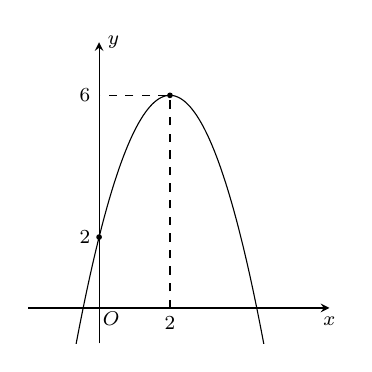
\begin{tikzpicture}[scale=0.45,font=\footnotesize,samples=200,>=stealth]
\draw[->] (-2,0)--(6.5,0) node[below]{$x$};
\draw[->] (0,-1)--(0,7.5) node[right]{$y$};
\node at (0,0) [below right=-2pt]{$O$};
\clip (-1,-1) rectangle (5.1,6.6);
\draw plot[domain=-1:5.1](\x,{-(\x)^2+4*\x+2});
\fill (0,2) circle(2.3pt) node[left]{$2$};
\fill (2,6) circle(2.3pt);
\draw[dashed] (2,0)node[below]{$2$}|-(0,6)node[left]{$6$};
\end{tikzpicture}
}
\loigiai{
Vì đồ thị là Parabol đi qua điểm $(2;6)$ và có trục đối xứng là $x=2$ nên ta có
\[\heva{&\dfrac{-b}{2a}=2 \\& 6=4a+2b+2} \Leftrightarrow \heva{&4a+b=0 \\&4a+2b=4} \Leftrightarrow \heva{&a=-1 \\& b=4.}\]
}
\end{bt}

% từ: cau-hoi/lop10/0D3_Ham_so_bac_hai_va_do_thi/0D3-2-2_Bang_bien_thien_tinh_don_dieu_max_min.tex
\begin{ex}%[0D3H2-2]%[ma:0225e689]
	 \immini[thm]{
	 Hàm số nào có bảng biến thiên như hình đưới đây?
	\choice 
		{$y=-x^2+4x-3$} 
		 {$y=2x^2-8x+7$}
		 {\True$y=x^2-4x+5$}
		 {$y=\dfrac{1}{2}x^2-2x+1$}
		 }{
		
\begin{tikzpicture}
				\tkzTabInit[nocadre=true,lgt=1,espcl=2.5,deltacl=0.5] 
					{$x$/0.7,$y$/2} 
					{$-\infty$,$2$,$+\infty$} 
				 \tkzTabVar{+/$+\infty$,-/$1$,+/$+\infty$}
			\end{tikzpicture}
		 }
	 \loigiai{
		Từ bảng biến  thiên ta loại $y=-x^2+4x-3$.\\
		Gọi $A\left(x_A; y_A\right)$ là đỉnh của  parabol, ta có:
		$\heva{&x_A=2\\&y_A=1}$.\\ 
		Suy  ra ta loại $y=2 x^2-8 x+7$ và $y=\dfrac{1}{2}x^2-2x+1$.
	} 
\end{ex}

% từ: cau-hoi/lop10/0D3_Ham_so_bac_hai_va_do_thi/0D3-2-2_Bang_bien_thien_tinh_don_dieu_max_min.tex
\begin{bt}%[0D3H2-2]%[Dự án đề kiểm tra Toán 10 HK1 NH24-25- Đoàn Minh Tâm]%[THPT Mạc Đĩnh Chi - TP.HCM]%[ma:dea3d434]
	Hãy lập bảng biến thiên của hàm số $y=3x^2+6x-9$. Từ đó tìm các khoảng đồng biến, nghịch biến và tập giá trị của hàm số $y=3x^2+6x-9$.
	\loigiai{
		Hàm số $y=3 x^2+6 x-9$ có đồ thị là $(P)$ với đinh $S(-1 ;-12)$.
		\begin{center}
			
\begin{tikzpicture}[>=stealth]
				\tkzTabInit[nocadre=false,lgt=1,espcl=2,deltacl=0.5]{$x$/.7 ,$y'$/.7,$y$/2}
				{$-\infty$ , $-1$ , $+\infty$}
				\tkzTabLine{ , - , $0$ , + , }
				\tkzTabVar{+/$+\infty$ , -/$-12$ , +/$+\infty$}
			\end{tikzpicture}
		\end{center}
		Hàm số đồng biến trên khoảng $(-1 ;+\infty)$, hàm số nghịch biến trên khoảng $(-\infty ;-1)$.\\
		Tập giá trị của hàm số $T=[-12 ;+\infty)$.
	}
\end{bt}

% từ: cau-hoi/lop10/0D3_Ham_so_bac_hai_va_do_thi/0D3-2-2_Bang_bien_thien_tinh_don_dieu_max_min.tex
\begin{bt}%[0D3V2-2]%[Dự án đề kiểm tra Toán 10 GHKI NH23-24 - Nguyễn Văn Sang]%[THPT Võ Văn Kiệt - Tp HCM]%[ma:afd553af]
	Cho hàm số $f(x)= \heva{&\dfrac{2 \sqrt{x+2}-3}{x-1} & \text { khi } x \geq 2 \\& x^2+m^2-2 m & \text { khi } x<2}$ với $m$ là tham số thực.\\
	Đặt $A=f(1)+f(2)$, xác định $m$ để $A$ đạt giá trị nhỏ nhất.
	\loigiai{
		Ta có
		\begin{itemize}
			\item $f(1)=m^2-2m+1$.
			\item $f(2)=\dfrac{2 \sqrt{2+2}-3}{2-1}=1$.
			\item $A=f(1)+f(2)=m^2-2m+1+1=(m-1)^2+1\geq 1, \forall m\in \mathbb{R}$.\\
			Vậy giá trị nhỏ nhất của $A=1$ khi $m-1=0 \Leftrightarrow m=1$.
		\end{itemize}
	}
\end{bt}

% từ: cau-hoi/lop10/0D3_Ham_so_bac_hai_va_do_thi/0D3-2-2_Bang_bien_thien_tinh_don_dieu_max_min.tex
\begin{bt}%[0D3H2-2]%[ma:4849c278]
	\immini
	{
		Cho đồ thị của hàm số bậc hai như hình bên.
		\begin{enumerate}
			\item Tìm toạ độ đỉnh của đồ thị.
			\item Tìm khoảng đồng biến và khoảng nghịch biến của hàm số.
			\item Tìm giá trị lớn nhất của hàm số.
			\item Tìm tập xác định và tập giá trị của hàm số.
		\end{enumerate}
	}
	{
		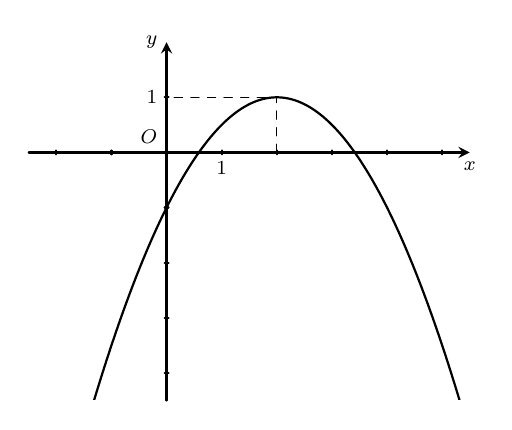
\begin{tikzpicture}[join=round, cap=round,>=stealth,thick, font = \footnotesize, scale = .7]
			\def \xmin{-2.5} 		\def \xmax{5.5}
			\def \ymin{-4.5}	\def \ymax{2}
			\draw[->] (\xmin,0)--(\xmax,0) node[below] {$x$}; 
			\draw[->] (0,\ymin)--(0,\ymax) node[left] {$y$}; 
			\fill (0,0) circle (1pt) node [above left] {$O$}; 
			\foreach \x in {-2,-1,1,2,3,4,5} 
			\draw (\x,1pt)--(\x,-1pt); 
			\foreach \y in {-4,-3,-2,-1,1} 
			\draw (1pt,\y)--(-1pt,\y);
			\path (1,0) node[below]{$1$}
			(0,1) node[left]{$1$}
			; 
			\draw[dashed,thin](2,0) |- (0,1);
			\begin{scope}
				\clip (\xmin+0.01,\ymin+0.01) rectangle (\xmax-0.01,\ymax-0.01); 
				\draw plot[samples=350,domain=\xmin+0.01:\xmax-0.01,smooth,variable=\x] (\x,{(-1/2)*(\x)^2 + 2*(\x) - 1});
			\end{scope}
		\end{tikzpicture}
	}
	\loigiai
	{
		\begin{enumerate}
			\item Toạ độ đỉnh của đồ thị hàm số là $I(2; 1)$.
			\item Hàm số đồng biến trên khoảng $(-\infty; 2)$ và nghịch biến trên khoảng $(2;+\infty)$.
			\item Hàm số có giá trị lớn nhất là $1$, đạt được khi $x=2$.
			\item Tập xác định của hàm số là $\mathbb{R}$. Tập giá trị của hàm số là $(-\infty; 1]$.
		\end{enumerate}
	}
\end{bt}

% từ: cau-hoi/lop10/0D3_Ham_so_bac_hai_va_do_thi/0D3-2-3_Do_thi_cua_ham_so_bac_hai.tex
\begin{ex}%[0D3N2-3]%[ma:3d2e8b24]
	\immini{Cho  đồ thị hàm số sau.
	Điểm thuộc đồ thị hàm  số mà có hoành độ bằng $2$ là
	 \choice
		{$(2;0)$} 
		{\True $(2;3)$} 
		{$(3;2)$} 
		{$(2;-3)$}}{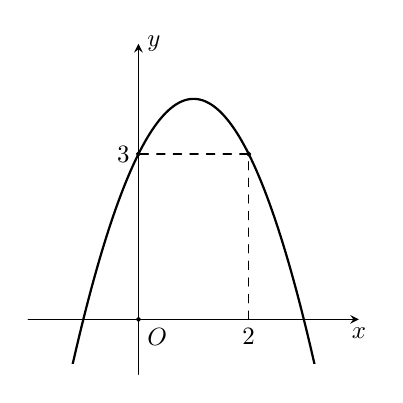
\begin{tikzpicture}[scale=0.7,>=stealth,line join=round,line cap=round,smooth,samples=450,declare function={xmin=-2; xmax=4; ymin=-1; ymax=5;}]
		 \path (0,0) node[below right]{$O$}
			(0,3) node[left]{$3$} 
			(2,0) node[below]{$2$}; 
		 \draw[->] (xmin,0)--(xmax,0) node[below]{$x$};
		 \draw[->] (0,ymin)--(0,ymax) node[right]{$y$};
		\clip  (xmin+.2,ymin+.2) rectangle (xmax-.2,ymax-.2);
		\draw[domain=xmin:xmax,smooth,thick,variable=\x,black] plot ({\x},{-\x*\x + 2*\x  + 3});
		\draw[dashed] (2,0) -- (2,3) --  (0,3);
		 \path[fill=black,draw] (0,3) circle (1pt);
		\path[fill=black,draw] (2,3) circle  (1pt);
		\path[fill=black,draw] (0,0)  circle (1pt);
	\end{tikzpicture}
		} 
	\loigiai{Dựa vào đồ thị ta thấy điểm thuộc đồ thị hàm số có hoành độ bằng $2$ là điểm  $(2;3)$.}
\end{ex}

% từ: cau-hoi/lop10/0D3_Ham_so_bac_hai_va_do_thi/0D3-2-3_Do_thi_cua_ham_so_bac_hai.tex
\begin{ex}%[0D3H2-3]%[ma:f367b437]
	\immini[thm]{ 
	Hàm số nào có đồ  thị như hình vẽ bên dưới?
	\choice 
		 {\True $y=-x^2+4x-3$}
		{$y=-x^2-4x-3$} 
		 {$y=-2x^2-x-3$}
		{$y=x^2-4x-3$} 
		 }{
		\begin{tikzpicture}[>=stealth,x=1.0cm,y=1.0cm,scale=0.8]
				\draw[->] (-1,0) -- (4,0) node[below] {\scriptsize  $x$};
				\draw[->] (0,-2.5) --  (0,2) node[right] {\scriptsize $y$};
				\draw[dashed,thin]  (0,1)--(2,1)--(2,0);
				 \draw (0,1) node[left]{\scriptsize $1$}
					(0,0)  node[below left]{\scriptsize O}
					 (2,0) node[below]{\scriptsize $2$};
				\draw[domain=0.2:3.8,samples=150] plot  (\x,{-(\x)^2+4*(\x)-3});
			\end{tikzpicture}
		} 
	 \loigiai{
		Đồ thị có  bề lõm quay xuống dưới nên $a<0$. Trục đối xứng $x=2$.\\
		Vậy đồ thị đã cho là đồ thị hàm số $y=-x^2+4x-3$. 
	 }
\end{ex}

% từ: cau-hoi/lop10/0D3_Ham_so_bac_hai_va_do_thi/0D3-2-3_Do_thi_cua_ham_so_bac_hai.tex
\begin{ex}%[0D3H2-3]%[ma:0b994c0e]
	\immini[thm]{Đồ  thị hình bên dưới là đồ thị của hàm số nào?
	\choice 
		{$y=2x^2-4x-2$} 
		 {$y=-x^2-2x+3$}
		 {\True$y=x^2-2x-1$}
		 {$y=x^2+2x-2$}
		 }{
		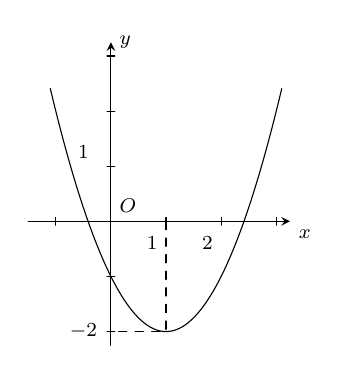
\begin{tikzpicture}[line cap=round,line join=round,font=\footnotesize,>=stealth,scale=0.7]
				 \tikzset{label style/.style={font=\footnotesize}}
				\draw[->] (-1.5,0)--(3.25,0)  node[below right] {$x$};
				\draw[->]  (0,-2.25)--(0,3.25) node[right] {$y$};
				\node (0,0)  [above right]{$ O $};
				\foreach \x in  {-1,1,2,3}
				\draw[shift={(\x,0)},color=black] (0pt,2pt) -- (0pt,-2pt); 
				\node at (.75,-0.4) {$1$}; 
				\node at (1.75,-0.4) {$2$}; 
				\foreach  \y in {-2,-1,1,2,3}
				\draw[shift={(0,\y)},color=black] (2pt,0pt) -- (-2pt,0pt); 
				\node at (-0.5,1.25)  {$1$};
				 \node at (-0.5,-2) {$-2$};
				 \draw[dashed](1,0)--(1,-2)--(0,-2);
				\draw [domain=-1.1:3.1,samples=100]  plot (\x,{(\x)*(\x)-2*(\x) - 1});
			\end{tikzpicture}
		 }
	 \loigiai{
		 Đồ thị cắt trục $Oy$ tại điểm có tung độ bằng $-1\Rightarrow c=-1$. Suy ra $y=ax^2+bx-1$.\\
		Đồ thị nhận $I\left(1;-2\right)$ làm đỉnh nên $\heva{&\dfrac{-b}{2a}=1\\ &-2=a\cdot 1^2+b\cdot 1-1}\Leftrightarrow\heva{&2a+b=0\\  &a+b=-1}\Leftrightarrow\heva{&a=1\\ &b=-2.}$\\
		Vậy $y=x^2-2x-1$. 
	} 
\end{ex}

% từ: cau-hoi/lop10/0D3_Ham_so_bac_hai_va_do_thi/0D3-2-3_Do_thi_cua_ham_so_bac_hai.tex
\begin{ex}%[0D3H2-3]%[ma:f70cb732]
	Nếu hàm số $y=ax^2+bx+c$ có $a>0$; $ b>0$ và $c<0$ thì  đồ thị hàm số của nó có dạng
	 \choice
		{\True 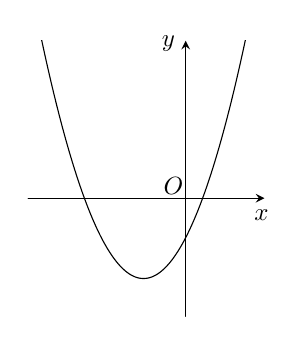
\begin{tikzpicture}[font=\footnotesize,line join=round,line cap=round,>=stealth]
		\tikzset{declare function={xmin=-2;  xmax=1; ymin=-1.5; ymax=2;
			 f (\x)=1.81*(\x)^2+1.94*(\x)-0.5;
			 },
			 smooth,samples=450
		 }
		\draw[->]  (xmin,0)--(xmax,0) node[shift={(-100:7pt)},font=\normalsize]{$ x $};
		\draw[->] (0,ymin)--(0,ymax) node[shift={(190:7pt)},font=\normalsize]{$  y $};
		\fill (0,0) node[shift={(135:7pt)},font=\normalsize]{$ O  $};
		\clip (xmin,ymin) rectangle (xmax,ymax); 
		\draw plot[domain=xmin:xmax] (\x,{f (\x)}); 
	\end{tikzpicture}
		} 
		{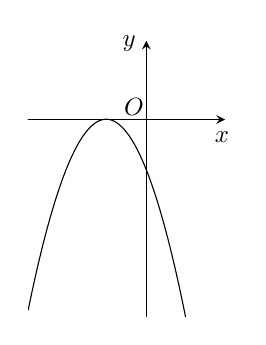
\begin{tikzpicture}[font=\footnotesize,line join=round,line cap=round,>=stealth]
		\tikzset{declare function={xmin=-1.5; xmax=1; ymin=-2.5;  ymax=1;
			f (\x)=-2.47*(\x)^2-2.52*(\x)-0.64; 
			 },
			smooth,samples=450 
		} 
		\draw[->]  (xmin,0)--(xmax,0) node[shift={(-100:7pt)},font=\normalsize]{$ x $};
		\draw[->] (0,ymin)--(0,ymax) node[shift={(190:7pt)},font=\normalsize]{$ y $}; 
		 \fill (0,0) node[shift={(135:7pt)},font=\normalsize]{$ O $};
		\clip  (xmin,ymin) rectangle (xmax,ymax);
		\draw  plot[domain=xmin:xmax] (\x,{f (\x)});
	\end{tikzpicture}
		} 
		{\begin{tikzpicture}[font=\footnotesize,line join=round,line cap=round,>=stealth]
		 \tikzset{declare function={xmin=-1.5; xmax=2.5; ymin=-2; ymax=2.5;
			 f (\x)=-1.3*(\x)^2+1.3*(\x)+1.6;
			 },
			 smooth,samples=450
		} 
		\draw[->] (xmin,0)--(xmax,0)  node[shift={(-100:7pt)},font=\normalsize]{$ x $};
		\draw[->] (0,ymin)--(0,ymax) node[shift={(190:7pt)},font=\normalsize]{$ y  $};
		\fill (0,0) node[shift={(135:7pt)},font=\normalsize]{$  O $};
		 \clip (xmin,ymin) rectangle (xmax,ymax);
		\draw plot[domain=xmin:xmax]  (\x,{f (\x)});
	\end{tikzpicture}
		} 
		{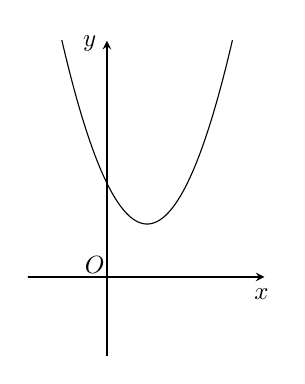
\begin{tikzpicture}[font=\footnotesize,line join=round,line cap=round,>=stealth]
		\tikzset{declare function={xmin=-1; xmax=2;  ymin=-1; ymax=3;
			f  (\x)=1.99*(\x)^2-2.03*(\x)+1.19;
			 },
			smooth,samples=450 
		} 
		\draw[->] (xmin,0)--(xmax,0) node[shift={(-100:7pt)},font=\normalsize]{$ x  $};
		\draw[->]  (0,ymin)--(0,ymax) node[shift={(190:7pt)},font=\normalsize]{$ y $};
		\fill (0,0) node[shift={(135:7pt)},font=\normalsize]{$ O  $};
		 \clip (xmin,ymin) rectangle (xmax,ymax);
		\draw plot[domain=xmin:xmax] (\x,{f  (\x)});
	\end{tikzpicture}
		 }
	\loigiai{ 
		Đồ thị hàm số $a>0$ nên bề lõm đồ thị quay lên và $c<0$ nên đồ thị cắt trục $Oy$ phía dưới $Ox $ nên  ta chọn
		\begin{center}
			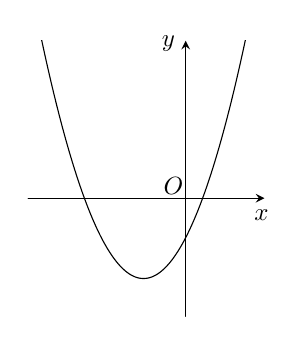
\begin{tikzpicture}[font=\footnotesize,line join=round,line cap=round,>=stealth]
					 \tikzset{declare function={xmin=-2; xmax=1; ymin=-1.5; ymax=2;
						f (\x)=1.81*(\x)^2+1.94*(\x)-0.5; 
						 },
						smooth,samples=450 
					 }
					\draw[->] (xmin,0)--(xmax,0) node[shift={(-100:7pt)},font=\normalsize]{$ x  $};
					\draw[->] (0,ymin)--(0,ymax) node[shift={(190:7pt)},font=\normalsize]{$ y  $};
					\fill  (0,0) node[shift={(135:7pt)},font=\normalsize]{$ O $};
					\clip  (xmin,ymin) rectangle (xmax,ymax);
					\draw  plot[domain=xmin:xmax] (\x,{f (\x)});
				\end{tikzpicture}
		\end{center}
	} 
\end{ex}

% từ: cau-hoi/lop10/0D3_Ham_so_bac_hai_va_do_thi/0D3-2-4_Bai_toan_ve_su_tuong_giao.tex
\begin{ex}%[0D3N2-4]%[ma:4c55d3b3]
	 \immini[thm]{Cho hàm số $y=ax^2+bx+c$ có đồ thị $(P)$ như hình vẽ. Khẳng định nào sau đây là \textbf{sai}?
	\choice 
		{Hàm  số đồng biến trên khoảng $(-\infty;3)$}
		{$(P)$ có  đỉnh là $I(3;4)$}
		{\True $(P)$ cắt trục tung tại điểm có tung độ  bằng $4$}
		{$(P)$ cắt trục hoành tại  hai điểm phân biệt}}
		 {
		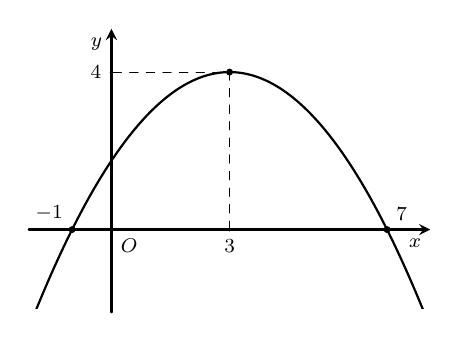
\begin{tikzpicture}[scale=0.5,line join=round,font=\footnotesize,line cap=round,>=stealth,thick]
				\tikzset{every  node/.style={scale=0.9}}
				\draw[->] (-2.1,0)--(8.1,0) node[below left] {$x$}; 
				 \draw[->] (0,-2.1)--(0,5.1) node[below left] {$y$};
				\draw (0,0) node  [below right] {$O$};
				\foreach \x/\nx in  {3/3}
				\draw[thin] (\x,1pt)--(\x,-1pt) node [below] {$\nx$}; 
				\foreach \y/\ny  in {4/4}
				\draw[thin] (1pt,\y)--(-1pt,\y) node  [left] {$\ny$};
				\draw[dashed,thin](3,0)--(3,4)--(0,4); 
				\begin{scope}
					 \clip (-2,-2) rectangle (8,5);
					 \draw[samples=200,domain=-2:8,smooth,variable=\x] plot (\x,{-0.25*(\x)^2+1.5*(\x)+1.75});
					\path (-1,0)  node[above left]{$-1$};
					\path (7,0) node[above  right]{$7$};
				\end{scope}
				\fill (3,4)  circle (2.5pt);
				\fill (-1,0)  circle (2.5pt);
				\fill (7,0)  circle (2.5pt);
			\end{tikzpicture}
		 }
	\loigiai{ 
		Dựa vào đồ thị ta thấy $(P)$ cắt  trục tung tại điểm có tung độ $y<4$.
	 }
\end{ex}

% từ: cau-hoi/lop10/0D3_Ham_so_bac_hai_va_do_thi/0D3-2-6_Toan_thuc_te_ung_dung_ham_so_bac_hai.tex
\begin{bt}%[0D3H2-6] % KIEM_TRA%[ma:8b4fe489]
		\immini{
			Nhà bác An có một mảnh đất nhỏ trồng rau có dạng hình thang vuông với các kích thước được cho như hình vẽ. Tìm $x$ để diện tích khoảng đất này không vượt quá $7{,}5 \mathrm{\,m}^2$.}
		{\vspace{-0.5cm}
			\begin{tikzpicture}[scale=1, font=\footnotesize, line join=round, line cap=round]
				\foreach \x\y\t in {0/0/A, 0/-2/B, 2.6/-2/C, 4/0/D}
				\coordinate (\t) at (\x,\y);
				\draw (C)--(D);
				\draw (A)--(B) node[pos=0.5,left]{$x-4 \;(\mathrm{m})$};
				\draw (C)--(B) node[pos=0.5,below]{$x-3 \;(\mathrm{m})$};
				\draw (A)--(D) node[pos=0.5,above]{$2x-5 \;(\mathrm{m})$};
				\path pic[draw,angle radius=4]{right angle=A--B--C};
				\path pic[draw,angle radius=4]{right angle=B--A--D};
		\end{tikzpicture}}
		\loigiai{
			Điều kiện của biến số $x$ là $\heva{&x-4>0\\&2x-5>0\\&x-3>0} \Leftrightarrow x>4$.\\
			Diện tích mảnh đất trồng rau của bác An là 
			$$S(x)=\dfrac{(2x-5)+(x-3)}{2}\cdot (x-4)=\dfrac{3}{2}x^2-10x+16 \mathrm{\;(m^2)}.$$
			Diện tích trồng rau đó không vượt quá $7{,}5 \mathrm{\,m}^2$ nghĩa là
			$$\dfrac{3}{2}x^2-10x+16  \leq  7{,}5 
			\Leftrightarrow \dfrac{3}{2}x^2-10x+\dfrac{17}{2}  \leq  0.$$
			Cho $\dfrac{3}{2}x^2-10x+\dfrac{17}{2} = 0 \Leftrightarrow \hoac{&x=1\\&x=\dfrac{17}{3}.}$\\
			Bảng xét dấu
			\begin{center}
				\begin{tikzpicture}
					\tkzTabInit[nocadre=true,lgt=1.2,espcl=2.,deltacl=0.4]
					{$x$/1, $f'(x)$/0.9}
					{$-\infty$, $1$, $4$, $\dfrac{17}{3}$, $+\infty$}
					\tkzTabLine{,+,0,-,,-,0,+,}
					\path (0.2,0) coordinate (t);
					\fill[pattern=north east lines]
					(T11) rectangle ($(N32)$);
					\draw ($(N31)$)--($(N32)$);
				\end{tikzpicture}
			\end{center}
			Vậy với $4 <x \leq \dfrac{17}{3}$ thì mảnh đất trồng rau của bác An không vượt quá $7{,}5 \mathrm{\,m}^2$.
		}
	\end{bt}

% từ: cau-hoi/lop10/0D6_Thong_ke/0D6-1-1_Tinh_va_uoc_luong_sai_so_tuyet_doi_tuong_doi.tex
\begin{ex}%[0D6H1-1][H]%[Nguyễn Văn Cường (Cường NV) - Dự án bài giảng K10 - K11]%[ma:a2832ffa]
Biết mảnh đất hình chữ nhật có chiều dài $x=23$ m $\pm 0{,}01$ m và chiều rộng $y = 15$ m $\pm 0{,}01$ m. Xét tính đúng sai của các khẳng định sau
\choiceTF[t]
{Độ dài lớn nhất của chiều dài hình chữ nhật là $23$ m}
{\True Chiều rộng của hình chữ nhật nằm trong khoảng $14{,}99$ m đến $15{,}01$ m}
{Chu vi của hình chữ nhật là $96$ m $\pm 0{,}01$ m}
{Diện tích của hình chữ nhật là $345$m $\pm 0{,}0001$ m}
\loigiai{
\begin{itemchoice}
\itemch Độ dài lớn nhất của chiều dài hình chữ nhật là $23{,}01$ m.
\itemch Do chiều rộng $y = 15$ m $\pm 0{,}01$ m nên chiều rộng của hình chữ nhật nằm trong khoảng $14{,}99$ m đến $15{,}01$ m.
\itemch Chu vi hình chữ nhật là
\[P = 2(x+y) = 2(23 + 15) \pm 2(0{,}01 + 0{,}01) = 96\,\text{m} \pm 0{,}04\,\text{m}.\]
\itemch Diện tích của hình chữ nhật là 
\[S = xy = (23 \pm 0{,}01) \cdot (15 \pm 0{,}01) = 23 \cdot 15 \pm (23 \cdot 0{,}01 + 15 \cdot 0{,}01 + 0{,}01^2) = 345\,\text{m} \pm 0{,}3801\,\text{m}.\]
\end{itemchoice}
}
\end{ex}

% từ: cau-hoi/lop10/0D7_Bat_phuong_trinh_bac_2_mot_an/0D7-1-3_Bai_toan_xet_dau_biet_BXD_do_thi.tex
\begin{bt}%[0D7N1-3]%[ID]%[Dự án đề kiểm tra HKII NH22-23- Nguyễn Văn Sang]%[THPT TRẦN QUANG KHẢI]%[ma:5091e2bb]
\immini
{
Dựa vào đồ thị của hàm số bậc hai trong hình vẽ, em hãy xét dấu của tam thức bậc hai $f(x)$.
}
{
\begin{tikzpicture}[>=stealth,x=1cm,y=1cm,scale=.75]
	\draw[->] (-5,0) -- (1.5,0) node[below] {$x$};
	\draw[->] (0,-2) -- (0,3) node[left] { $y$};
	\fill (0,0)circle (1.5pt) node[below left]{ $O$};
	\fill (-4,0)circle (1.5pt) node[below left]{$-4$};
	\fill (-1,0)circle (1.5pt) node[below left]{$-1$};
	\draw (-2.5,2.25)node[above]{$f(x)$};
	\draw[samples=150,smooth,domain=-4.5:-0.5] plot(\x,{-(\x)^2-5*\x-4});
\end{tikzpicture}
}
\loigiai{
	Dựa vào đồ thị hàm số $y=f(x)$ ta có bảng xét dấu như sau
\begin{center}
	
\begin{tikzpicture}
		\tkzTabInit[lgt=2,espcl=2,deltacl=0.5]
		{$x$/1 ,$f(x)$/1}
		{$-\infty$ , $-4$ , $-1$, $+\infty$}
		\tkzTabLine{,-,0,+,0,-,}
	\end{tikzpicture}
\end{center}
Vậy
\begin{itemize}
	\item  $f(x)>0$ với mọi $x\in \left(-4;-1 \right) $.
	\item  $f(x)<0$ với mọi $x\in \left(-\infty;-4\right)\cup \left(-1;+\infty\right) $.
	\item $f(x)=0$ tại $x=-1$ và $x=-4$.
\end{itemize}
}
\end{bt}

% từ: cau-hoi/lop10/0D7_Bat_phuong_trinh_bac_2_mot_an/0D7-1-3_Bai_toan_xet_dau_biet_BXD_do_thi.tex
\begin{bt}%[0D7H1-3]%[Tex hóa SGK CD-CT,T7/22, Tuấn Nguyễn]%Bài 1%[ma:15b6ecb8]
	Dựa vào đồ thị của hàm số bậc hai $y=f(x)$ sau đây, hãy xét dấu của tam thức bậc hai $f(x)$
	\begin{listEX}[2]
		\item \begin{tikzpicture}[scale=1,font=\footnotesize,line cap=round,line join=round,>=stealth]
			\def\a{1} \def\b{-3.5} \def\c{1.5} % Hệ số
			\def\xt{-1} \def\xp{4} \def\yt{2} \def\yd{-2} % x_trái, x_phải, y_trên, y_dưới (giới hạn)
			\draw[->] (\xt,0)--(\xp,0) node [below]{$x$};
			\draw[->] (0,\yd)--(0,\yt) node [left]{$y$};
			\node at (0,0) [below left]{$O$};
			\clip (\xt-0.1,\yd+0.1) rectangle (\xp-0.1,\yt-0.1);
			\draw[smooth,samples=300] plot(\x,{\a*(\x)^2+\b*(\x)+\c});
			\draw[fill=black] (.5,0) node[shift={(-90:.4)}]{$\tfrac{1}{2}$} circle(1pt);\draw[fill=black]  (3,0) node[shift={(-90:.4)}]{$3$} circle(1pt);
			\draw (3,1.5) node[shift={(180:.5)}]{$y=f(x)$};
		\end{tikzpicture}
		\item \begin{tikzpicture}[scale=.6,font=\footnotesize,line cap=round,line join=round,>=stealth]
			\def\a{-1/4} \def\b{2/4} \def\c{15/4} % Hệ số
			\def\xt{-4} \def\xp{6} \def\yt{5} \def\yd{-2} % x_trái, x_phải, y_trên, y_dưới (giới hạn)
			\draw[->] (\xt,0)--(\xp,0) node [below]{$x$};
			\draw[->] (0,\yd)--(0,\yt) node [left]{$y$};
			\node at (0,0) [below left]{$O$};
			\clip (\xt-0.1,\yd+0.1) rectangle (\xp-0.1,\yt-0.1);
			\draw[smooth,samples=300,domain=-3.5:5.2] plot(\x,{\a*(\x)^2+\b*(\x)+\c});
			\draw[fill=black]  (-3,0) node[shift={(-80:.4)}]{$-3$} circle(1pt);\draw[fill=black]  (5,0) node[shift={(-90:.4)}]{$5$} circle(1pt);
			\draw (4.5,-1) node[shift={(-90:.4)}]{$y=f(x)$};
		\end{tikzpicture}
		\item \begin{tikzpicture}[scale=.6,font=\footnotesize,line cap=round,line join=round,>=stealth]
			\def\a{1/3} \def\b{-6/3} \def\c{9/3} % Hệ số
			\def\xt{-1} \def\xp{6} \def\yt{5} \def\yd{-1} % x_trái, x_phải, y_trên, y_dưới (giới hạn)
			\draw[->] (\xt,0)--(\xp,0) node [below]{$x$};
			\draw[->] (0,\yd)--(0,\yt) node [left]{$y$};
			\node at (0,0) [below left]{$O$};
			\clip (\xt-0.1,\yd+0.1) rectangle (\xp-0.1,\yt-0.1);
			\draw[smooth,samples=300,domain=-.3:6] plot(\x,{\a*(\x)^2+\b*(\x)+\c});
			\draw[fill=black]  (3,0) node[shift={(-90:.4)}]{$3$} circle(1pt);
			\draw (1,3.5) node[shift={(0:.4)}]{$y=f(x)$};
		\end{tikzpicture}
		\item \begin{tikzpicture}[scale=1,font=\footnotesize,line cap=round,line join=round,>=stealth]
			\def\a{-1} \def\b{-2} \def\c{-1.5} % Hệ số
			\def\xt{-3} \def\xp{1} \def\yt{1} \def\yd{-3} % x_trái, x_phải, y_trên, y_dưới (giới hạn)
			\draw[->] (\xt,0)--(\xp,0) node [below]{$x$};
			\draw[->] (0,\yd)--(0,\yt) node [left]{$y$};
			\node at (0,0) [below left]{$O$};
			\clip (\xt-0.1,\yd+0.1) rectangle (\xp-0.1,\yt-0.1);
			\draw[smooth,samples=300,domain=-3.5:5.8] plot(\x,{\a*(\x)^2+\b*(\x)+\c});
			\draw (-2.5,-2.5) node[shift={(0:1)}]{$y=f(x)$};
		\end{tikzpicture}
	\end{listEX}
	\loigiai{
		\begin{enumerate}
			\item $f(x)$ dương trong hai khoảng $\left(-\infty;\dfrac{1}{2}\right)$ và $(3;+\infty)$, âm trong khoảng $\left(\dfrac{1}{2};3\right)$.
			\item $f(x)$ dương trong khoảng $(-3;5)$, âm trong hai khoảng $(-\infty;-3)$ và $(5;+\infty)$.
			\item $f(x)$ dương với mọi $x \ne 3$.
			\item $f(x)$ âm với mọi $x \in \mathbb{R}$.
		\end{enumerate}
	}
\end{bt}

% từ: cau-hoi/lop10/0D7_Bat_phuong_trinh_bac_2_mot_an/0D7-2-6_Bai_toan_co_tham_so.tex
\begin{ex}%[0D7N2-6]%[ma:1391103d]
	Có bao nhiêu giá trị nguyên âm của tham số $m$ để  hàm số $y=\sqrt{x^2-2mx-2m+3}$ có tập xác định là $\mathbb{R}$.
	 \choice
		{$4$} 
		 {$6$}
		{\True  $3$}
		{$5$} 
	 \loigiai{
		Hàm số $y=\sqrt{x^2-2mx-2m+3}$ có  tập xác định là $\mathbb{R}$ khi $x^2-2mx-2m+3 \geq 0$ với mọi $x \in \mathbb{R}$\\
		$\Leftrightarrow \heva{ 
		&\Delta' \leq  0\\
		 &a>0}
		\Leftrightarrow  \heva{
		 &m^2+2m-3 \leq 0\\
		&1>0} 
		\Leftrightarrow -3 \leq m \leq  1$.\\
		Do  $m$ nguyên âm nên $m \in\{-3;-2;-1\}$.\\
		 Vậy có $3$ giá trị nguyên âm của $m$ thỏa yêu cầu bài toán.
	} 
\end{ex}

% từ: cau-hoi/lop10/0D7_Bat_phuong_trinh_bac_2_mot_an/0D7-2-6_Bai_toan_co_tham_so.tex
\begin{ex}%[0D7V2-6]%[ma:163207e1]
	Cho $f(x)=x^2-2(m+1)x+4$ với $m$ là tham số thực. 
	\choiceTF 
		{\True $f(x)$ là tam thức bậc hai với mọi  giá trị của tham số $m$}
		{\True Khi $m=1$ thì hàm số $y=\sqrt{f(x)}$ có tập xác  định là $\mathbb{R}$}
		{Khi $m=-\dfrac{1}{2}$ thì  $f(x)<0,\forall x\in[-2;3]$}
		{Có $2$ giá trị nguyên  âm của tham số $m$ để $f(x)>0,\forall x\in\mathbb{R}$}
	 \loigiai{
		\begin{itemchoice}
			\itemch \textbf{Đúng}. 
			 \itemch \textbf{Đúng}. \\
			Với $m=1$ thì $y=\sqrt{f(x)}=\sqrt{x^2-4x+4}$ có ĐKXĐ  $x^2-4x+4\ge 0 \Leftrightarrow x\in \mathbb{R}$.
			\itemch  \textbf{Sai}. \\
			Với  $m=-\dfrac{1}{2}$ thì $f(x)=x^2-x+4<0 \Leftrightarrow x\in \varnothing$.
			 \itemch \textbf{Sai}. \\
			$f(x)>0,\forall x\in\mathbb{R} \Leftrightarrow \heva{&a>0  \\ &\Delta<0} \Leftrightarrow 4(m+1)^2-16<0 \Leftrightarrow -3<m<1$. \\
			Vậy có $3$ giá trị  nguyên $m\in\{-2;-1;0\}$.
		\end{itemchoice}
	 }
\end{ex}

% từ: cau-hoi/lop10/0D7_Bat_phuong_trinh_bac_2_mot_an/0D7-2-6_Bai_toan_co_tham_so.tex
\begin{bt}%[0D7V2-6]%[ma:219f3f33]
	Có bao nhiêu giá trị nguyên của tham số $m$, hàm  số $y=\sqrt{x^2-2mx+m-1}$ có tập xác định là $\mathbb{R}$?
	\loigiai{ 
		Để hàm số $y=\sqrt{x^2-2mx+m-1}$  có tập xác định là $\mathbb{R}$ thì \[x^2-2mx+m-1\ge 0,\,\forall x\in \mathbb{R}\Leftrightarrow\heva{&{a > 0} \\
		&{\Delta  \le 0}&}\Leftrightarrow\heva{&1>0\\&m^2-m+1\leq 0\;(*)}.\]
		 Vì $\left(m-\dfrac{1}{2}\right)^2+\dfrac{3}{4}>0,\,\forall x$ nên (*) vô nghiệm.\\
		Vậy không tồn tại giá trị của tham số $m$ để thoả mãn yêu cầu bài  toán.
	 }
\end{bt}

% từ: cau-hoi/lop10/0D7_Bat_phuong_trinh_bac_2_mot_an/0D7-3-2_Phuong_trinh_can.tex
\begin{ex}%[0D7V3-2]%[ma:ec08b1cd]
	Cho phương trình $\sqrt{2x^2 +  x - 6} = x+2\quad (1)$. Khi đó
	 \choiceTF
		{Bình phương hai vế của phương trình $(1)$ ta được phương trình $x^2 + 3x  - 10 = 0$}
		{Điều kiện  xác định của phương trình là $x\ge 3$}
		{\True Phương trình $(1)$ có hai nghiệm  phân biệt}
		 {\True Tổng các nghiệm của phương trình $(1)$ là $3$}
	 \loigiai{
		Bình phương hai vế của phương trình $(1)$ ta được 
		 \[
		2x^2 + x - 6 = (x+2)^2 \Leftrightarrow x^2 - 3x - 10 = 0 \Leftrightarrow \hoac{&x=5\\ & x  = -2.}
		\] 
		Thử lại  ta thấy $x=5$ và $x=-2$ đều thoả mãn. Vậy
		\begin{itemchoice}
			\itemch Bình phương hhai vế và thu gọn, ta được  phương trình $x^2 - 3x - 10 = 0$.
			 \itemch Phương trình xác định khi và chỉ khi
			\[ 
			 2x^2 + x - 6 \ge 0 \Leftrightarrow (x+2)(x-3)\ge 0 \Leftrightarrow \hoac{&x\ge 3\\ &x\le -2.}
			\] 
			\itemch Phương trình có hai nghiệm $-2$ và $5$. 
			\itemch  Ta có tổng các nghiệm là $5 + (-2) = 3$.
		\end{itemchoice}
	} 
\end{ex}

% từ: cau-hoi/lop10/0D7_Bat_phuong_trinh_bac_2_mot_an/0D7-3-3_Phuong_trinh_can_thuc_co_tham_so.tex
\begin{bt}%[0D7V3-3]%[ma:794f4560]
	Cho bất  phương trình $4\sqrt{(x+1)(3-x)}\le x^2-2x+m-3$. Có bao nhiêu giá trị nguyên của tham số $m\in (-2022;2023]$ để bất phương trình nghiệm đúng với $\forall x\in [-1;3]$?
	 \shortans{2012}
	 \loigiai{
		Với mọi $x\in [-1;3]$ ta  có $(x+1)(3-x)=-x^2+2x+3\ge 0$.\\
		Đặt $t=\sqrt{(x+1)(3-x)} \ge 0$, đồng  thời $\sqrt{(x+1)(3-x)}\le\dfrac{x+1+3-x}{2}=2$. Do đó, $t\in[0;2]$.\\
		Khi  đó bất phương trình trở thành $t^2+4t-m\le 0\Leftrightarrow m\ge t^2+4t$ với $t\in [0;2]$.\\
		Với $t\in [0;2]$ ta có  $0\le t^2+4t\le 12$.\\
		Do đó, $m\ge  12$.\\
		Vậy số giá trị nguyên của tham số $m$ là $2023-12+1=2012$. 
	 }
\end{bt}

% từ: cau-hoi/lop10/0D8_Dai_so_to_hop/0D8-3-2_Khai_trien_mot_nhi_thuc_Newton.tex
\begin{bt}%[0D8H3-2]%[ma:efdc8c9f]
	Khai triển  các đa thức sau:
	\begin{multicols}{2}
		\begin{enumerate}[a)]
			 \item $(x+1)^{5}$
			 \item $(x-1)^{5}$
			 \item $(x+2)^{5}$
			\item  $(2x+y)^{5}$
			 \item $(x-3y)^{5}$
			 \item $(2x+3y)^{5}$
		\end{enumerate}
	\end{multicols}
	\loigiai{ 
		\begin{enumerate}[a)]
			\item $(x+1)^{5}\\ 
			= \mathrm{C}_5^0 x^5  1^0 + \mathrm{C}_5^1 x^4 1^1 + \mathrm{C}_5^2 x^3 1^2 + \mathrm{C}_5^3 x^2 1^3 + \mathrm{C}_5^4 x^1 1^4 + \mathrm{C}_5^5 x^0 1^5\\
			 = x^{5}+5x^{4}+10x^{3}+10x^{2}+5x+1$.
			\item $(x-1)^{5}\\ 
			= \mathrm{C}_5^0 x^5 (-1)^0 + \mathrm{C}_5^1 x^4 (-1)^1 + \mathrm{C}_5^2 x^3 (-1)^2 +  \mathrm{C}_5^3 x^2 (-1)^3 + \mathrm{C}_5^4 x^1 (-1)^4 + \mathrm{C}_5^5 x^0 (-1)^5\\
			= x^{5}-5x^{4}+10x^{3}-10x^{2}+5x-1$. 
			\item  $(x+2)^{5}\\
			= \mathrm{C}_5^0 x^5  2^0 + \mathrm{C}_5^1 x^4 2^1 + \mathrm{C}_5^2 x^3 2^2 + \mathrm{C}_5^3 x^2 2^3 + \mathrm{C}_5^4 x^1 2^4 + \mathrm{C}_5^5 x^0 2^5\\
			= 1 \cdot x^5 \cdot  1 + 5 \cdot x^4 \cdot 2 + 10 \cdot x^3 \cdot 4 + 10 \cdot x^2 \cdot 8 + 5 \cdot x \cdot 16 + 1 \cdot 1 \cdot 32\\
			=  x^{5}+10x^{4}+40x^{3}+80x^{2}+80x+32$.
			\item $(2x+y)^{5}\\ 
			= \mathrm{C}_5^0 (2x)^5 y^0 + \mathrm{C}_5^1 (2x)^4 y^1 + \mathrm{C}_5^2 (2x)^3 y^2 + \mathrm{C}_5^3 (2x)^2 y^3 + \mathrm{C}_5^4 (2x)^1 y^4 + \mathrm{C}_5^5 (2x)^0 y^5\\ 
			= 1 \cdot 32x^5 \cdot 1 + 5 \cdot 16x^4 \cdot y + 10 \cdot 8x^3 \cdot y^2 +  10 \cdot 4x^2 \cdot y^3 + 5 \cdot 2x \cdot y^4 + 1 \cdot 1 \cdot y^5\\
			=  32x^{5}+80x^{4}y+80x^{3}y^{2}+40x^{2}y^{3}+10xy^{4}+y^{5}$.
			\item $(x-3y)^{5}\\ 
			= \mathrm{C}_5^0 x^5 (-3y)^0 + \mathrm{C}_5^1 x^4 (-3y)^1 + \mathrm{C}_5^2 x^3 (-3y)^2 + \mathrm{C}_5^3 x^2  (-3y)^3 + \mathrm{C}_5^4 x^1 (-3y)^4 + \mathrm{C}_5^5 x^0 (-3y)^5\\
			 = 1 \cdot x^5 \cdot 1 + 5 \cdot x^4 \cdot (-3y) + 10 \cdot x^3 \cdot (9y^2) + 10 \cdot x^2 \cdot (-27y^3) + 5 \cdot x \cdot (81y^4) + 1 \cdot 1 \cdot (-243y^5)\\
			 = x^{5}-15x^{4}y+90x^{3}y^{2}-270x^{2}y^{3}+405xy^{4}-243y^{5}$.
			\item $(2x+3y)^{5}\\ 
			= \mathrm{C}_5^0 (2x)^5 (3y)^0 + \mathrm{C}_5^1 (2x)^4 (3y)^1 + \mathrm{C}_5^2 (2x)^3 (3y)^2 + \mathrm{C}_5^3 (2x)^2 (3y)^3 + \mathrm{C}_5^4  (2x)^1 (3y)^4 + \mathrm{C}_5^5 (2x)^0 (3y)^5\\= 1 \cdot 32x^5 \cdot 1 + 5 \cdot 16x^4 \cdot 3y + 10 \cdot 8x^3 \cdot 9y^2 + 10 \cdot 4x^2 \cdot 27y^3 + 5 \cdot 2x \cdot 81y^4 + 1 \cdot 1 \cdot 243y^5\\
			= 32x^{5}+240x^{4}y+720x^{3}y^{2}+1080x^{2}y^{3}+810xy^{4}+243y^{5}$. 
		\end{enumerate}
	} 
\end{bt}

% từ: cau-hoi/lop10/0D8_Dai_so_to_hop/0D8-3-2_Khai_trien_mot_nhi_thuc_Newton.tex
\begin{bt}%[0D8V3-2]%[Dự án đề kiểm tra HKII NH22-23-Võ Thị Thùy Trang]%[THPT CU CHI]%[ma:c996795e]
	Khai triển và rút gọn biểu thức $P=(\sqrt{2}-\sqrt{5})^4+(\sqrt{2}+\sqrt{5})^4$.
	\loigiai{
		\begin{itemize}
			\item $\left(a+b\right)^4=a^4+4a^3b+6a^2b^2+4ab^3+b^4$
			\item $\left(a-b\right)^4=a^4-4a^3b+6a^2b^2-4ab^3+b^4$
			\item $\left(a-b\right)^4+\left(a+b\right)^4=2a^4+12a^2b^2+2b^4$
			\item $P=(\sqrt{2}-\sqrt{5})^4+(\sqrt{2}+\sqrt{5})^4=2\cdot \sqrt{2}^4+12\cdot \sqrt{2}^2\cdot \sqrt{5}^2+2\cdot \sqrt{5}^4=178$.
	\end{itemize}}
\end{bt}

% từ: cau-hoi/lop10/0H4_He_thuc_luong_trong_tam_giac/0H4-1-1_Xet_dau_cua_bieu_thuc_luong_giac.tex
\begin{ex}%[0H4N1-1]%[ma:ddc31bf4]
	 Chọn khẳng định đúng trong các khẳng định sau
	\choice { $\sin(180^\circ-x)=-\sin x$}{ $\cos(180^\circ-x)=-\sin x$}{  $\tan(180^{\circ}-x)=\cot x$}{\True $\cos(180^{\circ}-x)=-\cos x$}
	\loigiai{ 
		Công thức  lượng giác cơ bản là $\cos(180^{\circ}-x)=-\cos x$.
	} 
\end{ex}

% từ: cau-hoi/lop10/0H4_He_thuc_luong_trong_tam_giac/0H4-1-2_Tinh_cac_gia_tri_luong_giac.tex
\begin{bt}%[0H4V1-2]%[ma:afb2a128]
% nguon: Archive/2024/SP-K10-K11-LyVanHoang_TVN-023/11. C1-LuongGiac-lvhoang_TVN-023/dataC1K11/Bai-1-Dang-7-GTLG-GocLienQuanDacBiet.tex #1718
[MĐ3]
	Tính
	\begin{enumerate}
		\item $A=\sin ^2 5^{\circ}+\sin ^2 10^{\circ}+\sin ^2 15^{\circ}+\ldots+\sin ^2 85^{\circ}$ ($17$ số hạng).
		\item $B=\cos 5^{\circ}+\cos 10^{\circ}+\cos 15^{\circ}+\ldots+\cos 175^{\circ}$ ($35$ số hạng).
	\end{enumerate}
	\loigiai{
		\begin{enumerate}
			\item Vận dụng $\sin \left(90^{\circ}-\alpha\right)=\cos \alpha$.\\
			Ta có $\sin 85^{\circ}=\cos 5^{\circ}$,  $\sin 80^{\circ}=\cos 10^{\circ}$, $\sin 75^{\circ}=\cos 15^{\circ}, \ldots, \sin 50^{\circ}=\cos 40^{\circ}$.
			\begin{eqnarray*}
				A & =&\left(\sin ^2 5^{\circ}+\cos ^2 5^{\circ}\right)+\left(\sin ^2 10^{\circ}+\cos ^2 10^{\circ}\right)+\ldots+\left(\sin ^2 40^{\circ}+\cos ^2 40^{\circ}\right)+\sin ^2 45^{\circ} \\
				& =&\underbrace{1+1+\ldots+1}_{\text {8 số 1 }}+\left(\dfrac{\sqrt{2}}{2}\right)^2=\dfrac{17}{2} .
			\end{eqnarray*}
			\item Vận dụng $\cos \left(180^{\circ}-\alpha\right)=-\cos \alpha$.\\
			Ta có $\cos 175^{\circ}=-\cos 5^{\circ}, \cos 170^{\circ}=-\cos 10^{\circ}$, $\cos 165^{\circ}=-\cos 15^{\circ}, \ldots, \cos 95^{\circ}=-\cos 85^{\circ}$.
			\begin{eqnarray*}
				B&=&\left(\cos 5^{\circ}+\cos 175^{\circ}\right)+\left(\cos 10^{\circ}+\cos 170^{\circ}\right)+\ldots+\left(\cos 85^{\circ}+\cos 95^{\circ}\right)+\cos 90^{\circ}\\
				&=&\underbrace{0+0+\ldots+0}_{17 \text { số } 0}+\cos 90^{\circ}=0.
			\end{eqnarray*}
		\end{enumerate} 
	}
\end{bt}

% từ: cau-hoi/lop10/0H4_He_thuc_luong_trong_tam_giac/0H4-2-2_Bai_toan_co_dung_cong_thuc_dien_tich.tex
\begin{bt}%[0H4V2-2]%[ma:8b34a15c]
	Cho tam giác $ABC$ có hai trung tuyến $BM$  và $CN$ hợp với nhau một góc $120^{\circ}$. Biết $BM=12$, $CN=15$. Tính chu vi của tam giác $ABC$ (kết quả là tròn đến hàng đơn vị).
	\begin{center}
		\begin{tikzpicture}[declare function={a = 5; goc = 65; b = 0.65*a;}]
				 \path
					 (goc:b) coordinate (A)
					(0,0) coordinate (B) 
					(a,0) coordinate (C); 
				\path (barycentric cs:A=1,B=1,C=1)  coordinate (G);
				\path  ($(A)!0.5!(B)$) coordinate (N);
				 \path ($(A)!0.5!(C)$) coordinate (M);
				\foreach \x/\y/\z in {B/G/C}{ 
					\path (\y) pic[draw,angle  radius=20pt,angle eccentricity=0.5,"$120^\circ$"]{angle = \x--\y--\z};
				 }
				\draw (A)--(B)--(C)--cycle; 
				\draw  (M)--(B)
					 (C)--(N);
				\foreach  \t/\g in {A/90,B/-90,C/-90,M/60,N/120,G/90}{
					\draw[fill=white] (\t) circle (1pt) node[shift={(\g:7pt)},font=\scriptsize]{$  \t $};
				} 
			\end{tikzpicture}
	\end{center}
	\loigiai{ 
		\begin{itemize}
			\item Gọi $BM\cap CN=G \Rightarrow G$ là trọng tâm  của tam giác $ABC$.
			\[\Rightarrow GB=\dfrac{2}{3}  BM=8,~ GC=\dfrac{2}{3} CN=10\Rightarrow GM=4,~ GN=5.\]
			Áp dụng  định lý cos trong tam giác $GBC$ có
			\[BC^2=GB^2+GC^2-2GB\cdot GC\cdot \cos 120^{\circ}=244\Rightarrow BC=2\sqrt{61}.\] 
			\item  Ta có $\widehat{BGN}=180^{\circ}-\widehat{BGC}=60^{\circ}$, $\widehat{MGC}=180^{\circ}-\widehat{BGC}=60^{\circ}$.\\
			Áp dụng định lý côsin,  ta được
			\[BN^2=GB^2+GN^2-2GB\cdot GN\cdot \cos 60^{\circ}=49\Rightarrow BN=7\Rightarrow  AB=2BN=14.\]
			\[MC^2=GM^2+GC^2-2GM\cdot GC\cdot \cos 60^{\circ}=76\Rightarrow MC=2\sqrt{19} \Rightarrow  AC=2MC=4\sqrt{19}.\]
		\end{itemize}
		Vậy chu vi của  tam giác $ABC$ là $AB+BC+CA=14+2\sqrt{61}+4\sqrt{19}=47{,}06\approx 47$.
	} 
\end{bt}

% từ: cau-hoi/lop10/0H5_Vecto_chua_xet_toa_do/0H5-2-6_Toan_thuc_te_ap_dung_tong_hieu_vecto.tex
\begin{bt}%[0H5V2-6]%[Đề ôn tập số 02-Tổng hiệu hai véc-tơ]%[Nguyễn Trung Kiên, dự án BG10]%[ma:b65f862b]
	\immini
	{Hai tàu cao tốc cùng xuất phát từ cùng một bến $A$ và chuyển động thẳng đều theo hai hướng. Tàu thứ nhất chạy với vận tốc là $18$ hải lý/giờ, tàu thứ hai chạy với vận tốc $16$ hải lý/giờ (một hải lý bằng $1{,}852$ km). Sau $2$ giờ, tàu thứ nhất đến vị trí $B$, tàu thứ hai đến vị trí $C$ và góc $\widehat{BAC}=50^\circ$. Tính $\left|\overrightarrow{AB} -\overrightarrow{AC}\right|$ (làm tròn đến hàng đơn vị theo đơn vị hải lý).}
	{\begin{tikzpicture}[font=\footnotesize, line join=round, line cap=round, >=stealth, scale=1]
			\def\a{4.5}
			\path (0,0) coordinate(A)
			(0:\a) coordinate(B)
			(50:{8/9*\a}) coordinate(C);
			\draw[->] (A)--(B);
			\draw[->] (A)--(C);
			\draw (B)--(C);
			\path (0,0) node{\hypersetup{hidelinks}\href{NhomToanLaTeX}{ }};
			\path pic["$50^\circ$" rotate=15, draw, angle radius=0.9 cm]{angle=B--A--C};
			\foreach \i/\j in {A/180, B/-90, C/90} \fill (\i) node[shift={(\j:3mm)}]{$\i$} circle(1pt);
	\end{tikzpicture}}
	\shortans{29}
	\loigiai{
		Do hai tàu chuyển động thẳng đều nên $\overrightarrow{AB}$ cùng hướng với véc-tơ vận tốc $\overrightarrow{v}_1$ của tàu thứ nhất, $\overrightarrow{AC}$ cùng hướng với véc-tơ vận tốc $\overrightarrow{v}_2$ của tàu thứ hai. Ta có
		\begin{itemize}
			\item $AB=2\left|\overrightarrow{v}_1\right| = 36$ hải lý.
			\item $AC=2\left|\overrightarrow{v}_2\right| = 32$ hải lý.
		\end{itemize}
		Khi đó $\left|\overrightarrow{AB} -\overrightarrow{AC}\right| = \left|\overrightarrow{CB}\right| = BC$.\\
		Tam giác $ABC$, có $$BC=\sqrt{AB^2+AC^2-2AB\cdot AC\cdot \cos\widehat{BAC}} = \sqrt{36^2+32^2-2\cdot 36\cdot 32 \cdot \cos{50^\circ}}\approx 29.$$
		Vậy $\left|\overrightarrow{AB} -\overrightarrow{AC}\right| = \left|\overrightarrow{CB}\right| = BC \approx 29$ hải lý.}
\end{bt}

% từ: cau-hoi/lop10/0H9_Phuong_phap_toa_do_trong_mat_phang/0H9-1-3_Toa_do_diem_va_vecto_tren_he_truc_Oxy.tex
\begin{bt}%[0H9H1-3]%[ma:06dd9f89]
	Trong mặt phẳng toạ độ $Oxy$, cho tứ giác $ABCD$ có $A(x_A;y_A)$, $B(x_B;y_B)$, $C(x_C;y_C)$, $D(x_D;y_D)$. Chứng minh tứ giác $ABCD$ là hình bình hành khi và chỉ khi $x_A+x_C=x_B+x_D$ và $y_A+y_C=y_B+y_D$.
	\loigiai{
		Tứ giác $ABCD$ là hình bình hành khi và chỉ khi
		$$
		\overrightarrow{AB}=\overrightarrow{DC} \Leftrightarrow \heva{&x_B-x_A=x_C-x_D\\&y_B-y_A=y_C-y_D} \Leftrightarrow \heva{&x_B+x_D=x_C+x_A\\&y_B+y_D=y_C+y_A.}
		$$
	}
\end{bt}

% từ: cau-hoi/lop10/0H9_Phuong_phap_toa_do_trong_mat_phang/0H9-1-3_Toa_do_diem_va_vecto_tren_he_truc_Oxy.tex
\begin{bt}%[0H9H1-3]%[Tex hóa SGK CD-CT,T7/22, Lê Minh Thiện Anh]%[ma:af6a5b57]
	Cho ba điểm $A(1;1)$, $B(2;4)$, $C(4;4)$.
	\begin{enumerate}
		\item Tìm tọa độ điểm $D$ sao cho $ABCD$ là một hình bình 	hành.
		\item Tìm tọa độ giao điểm hai đường chéo của hình bình hành $ABCD$.
	\end{enumerate}
	\loigiai{
		\begin{enumerate}
			\item $ABCD$ là hình bình hành $\Leftrightarrow \overrightarrow{AB}=\overrightarrow{DC}$.\\
			Đặt toạ độ của $D(x_D;y_D)$, ta có $\overrightarrow{AB}=\overrightarrow{DC} \Leftrightarrow \heva{&2-1=4-x_D\\&4-1=4-y_D} \Leftrightarrow \heva{&x_D=3\\&y_D=1.}$\\
			Vậy $D(3;1)$.
			\item Gọi $M$ là giao điểm hai đường chéo của hình bình hành $ABCD$.\\
			Ta có $M$ là trung điểm $AC$, suy ra $M(2{,}5;2{,}5)$.
		\end{enumerate}
	}
\end{bt}

% từ: cau-hoi/lop10/0H9_Phuong_phap_toa_do_trong_mat_phang/0H9-2-2_Tim_goc_nho_tich_vo_huong.tex
\begin{bt}%[0H9N2-2]%[Dự án đề kiểm tra HKII NH22-23 - Thành Đức Trung]%[Sở Bắc Giang]%[ma:ff898f8a]
Cho hai véc-tơ $\overrightarrow{a}=(3;1)$, $\overrightarrow{b}=(2;4)$. Tính góc giữa hai véc-tơ $\overrightarrow{a}$ và $\overrightarrow{b}$.
\loigiai
{
Ta có $\cos \left(\overrightarrow{a},\overrightarrow{b}\right)=\dfrac{\overrightarrow{a}\cdot\overrightarrow{b}}{\left|\overrightarrow{a}\right|\cdot\left|\overrightarrow{b}\right|}=\dfrac{3\cdot2+1\cdot4}{\sqrt{3^2+1^2}\cdot\sqrt{2^2+4^2}}=\dfrac {\sqrt 2}{2} \Rightarrow \left(\overrightarrow{a},\overrightarrow{b}\right)=45^{\circ}$. \\
Vậy góc giữa hai véc-tơ $\overrightarrow{a}$ và $\overrightarrow{b}$ là $45^{\circ}$.
}
\end{bt}

% từ: cau-hoi/lop10/0H9_Phuong_phap_toa_do_trong_mat_phang/0H9-3-2_Phuong_trinh_duong_thang.tex
\begin{bt}%[0H9H3-2]%[ma:55083182]
Trong mặt phẳng toạ độ, cho hai điểm $A(-1 ; 0)$ và $B(3 ; 1)$.
\begin{enumerate}[a)]
\item Viết phương trình đường tròn tâm $A$ và đi qua $B$.
\item Viết phương trình tồng quát của đường thẳng $A B$.
\item Viết phương trình đường tròn tâm $O$ và tiếp xúc với đường thẳng $AB$.
\end{enumerate}
\loigiai{
\begin{enumerate}[a)]
\item Viết phương trình đường tròn tâm $A$ và đi qua $B$.\\
Phương trình đường tròn $(C)$ có tâm $A(-1 ; 0)$ và bán kính\\ $R=AB=\sqrt{(3+1)^2+(1-0)^2}=\sqrt{17}$:
		\[(C): (x+1)^2+y^2=17\]
\item Viết phương trình tổng quát của đường thẳng $AB$.\\
		Ta có $\overrightarrow{AB}=(4;1)$.\\
		Phương trình tổng quát $AB$ đi qua điểm $A(-1 ;0)$ và có một vectơ pháp tuyến là $\overrightarrow{n}=(1 ; -4)$:\\
		\[d: 1(x+1)-4(y-0)=0\]
		\[d: x-4y+1=0\]
\item Viết phương trình đường tròn tâm $O$ và tiếp xúc với đường thẳng $AB$.\\
	Ta có $d(O,AB)=\dfrac{\left| 0 -4.0+1 \right|}{\sqrt{1^2+(-4)^2}}=\dfrac{\sqrt{17}}{17}$.\\
	Phương trình đường tròn tâm $O(0;0)$ có bán kính $R=d(O,AB)=\dfrac{\sqrt{17}}{17}$:\\
	\[(C): (x-0)^2+(y-0)^2=\dfrac{1}{17}\]
	\[(C): x^2+y^2=\dfrac{1}{17}\]
\end{enumerate}
}
\end{bt}

% từ: cau-hoi/lop10/0H9_Phuong_phap_toa_do_trong_mat_phang/0H9-3-2_Phuong_trinh_duong_thang.tex
\begin{bt}%[0H9H3-2]%[Dự án đề kiểm tra GHKII NH22-23- Thầy Hóa]%[THPT Tây Thạnh]%[ma:b0f7e4dd]
Trong mặt phẳng $Oxy$, cho tam giác $ABC$ có tọa độ các đỉnh là $A(2;3)$, $B(4;5)$ và $C(6;5)$.
\begin{enumerate}
	\item Tính độ dài đoạn thẳng $AB$ và số đo góc $B$ trong tam giác $ABC$.
	\item Tìm tọa độ điểm $D\left(m;m^2-6m-4\right)$ sao cho tứ giác $ABCD$ là hình thang có hai đáy là $BC$, $AD$.
	\item Lập phương trình tham số của trung tuyến $AM$.
\end{enumerate}
\loigiai{
\begin{enumerate}
	\item Ta có $\begin{aligned}[t]
		&\overrightarrow{AB}=(2;2)\Rightarrow AB=\sqrt{2^2+2^2}=2\sqrt{2};\\
		&\overrightarrow{AC}=(4;2)\Rightarrow AC=\sqrt{4^2+2^2}=2\sqrt{5};\\
		&\overrightarrow{BC}=(2;0)\Rightarrow BC=\sqrt{2^2+0^2}=2.
	\end{aligned}$\\
	Áp dụng định lý cô-sin, ta có
	\allowdisplaybreaks
	\begin{eqnarray*}
		\cos B&=&\dfrac{BC^2+AB^2-AC^2}{2\cdot BC\cdot AB}\\
		&=&\dfrac{4+8-20}{2\cdot 2\cdot 2\sqrt{2}}\\
		&=&\dfrac{-1}{\sqrt{2}}.
	\end{eqnarray*}
	Suy ra $\widehat{B}=135^\circ$.
	\item Ta có $\overrightarrow{AD}=\left(m-2;m^2-6m-7\right)$.\\
	Vì $ABCD$ là hình thang có $BC\parallel AD$ nên $\overrightarrow{AD}=k\overrightarrow{BC}\ (k\neq 0)$. Do đó
	\[m^2-6m-7=0\Leftrightarrow \hoac{&m=-1\\&m=7.} \]
	\begin{itemize}
		\item Với $m=-1\Rightarrow D(-1;3)$.
		\item Với $m=7\Rightarrow D(7;3)$.
	\end{itemize}
	Vậy có 2 điểm $D$ thỏa mãn yêu cầu bài toán là $D(-1;3)$ và $D(7;3)$.
	\item Vì $M$ là trung điểm của $BC$ nên $M(5;5)$.\\
	Ta có $\overrightarrow{AM}=(3;2)$. Phương trình tham số của đường thẳng $AM$
	\[AM\colon\heva{&x=2+3t\\&y=3+2t}\ (t\in\mathbb{R}). \]
\end{enumerate}
}
\end{bt}

% từ: cau-hoi/lop10/0H9_Phuong_phap_toa_do_trong_mat_phang/0H9-3-4_Bai_toan_ve_goc_giua_hai_duong_thang.tex
\begin{ex}%[0H9Y3-4]%[ma:b9da320d]
	Người ta quy ước góc giữa hai đường  thẳng song song hoặc trùng nhau là
	 \choice
		 {$180^\circ$}
		 {$120^\circ$}
		 {$90^\circ$}
		{\True  $0^\circ$}
	\loigiai{ 
		Góc giữa hai  đường thẳng song song hoặc trùng nhau là $0^\circ$.
	 }
\end{ex}

% từ: cau-hoi/lop10/0H9_Phuong_phap_toa_do_trong_mat_phang/0H9-3-7_Bai_toan_dung_cho_tam_giac_tu_giac.tex
\begin{ex}%[0H9H3-7]%[0H9H3-4]%[0H9H2-4]%[0H9N1-3]%[ma:a6a4a6db]
	Trong mặt phẳng tọa độ $Oxy$, cho ba điểm $A(1;-1)$, $B(5;-3)$ và $C(2;0)$. Xét tính đúng  sai của mỗi khẳng định dưới đây.
	 \choiceTF
		{\True  Độ dài của đoạn thẳng $AB=\sqrt{20}$}
		{Tọa độ trọng tâm của tam giác $ABC$ là $G\left(\dfrac{8}{3};\dfrac{4}{3}\right)$} 
		 {Tam giác $ABC$ là tam giác vuông tại $A$}
		{\True Diện tích của tam giác $ABC$ là  $3$ (đvdt)}
	\loigiai{ 
		\begin{itemchoice}
			\itemch \textbf{Đúng}. Vì $\overrightarrow{AB}=(4;-2)\Rightarrow AB=\sqrt{4^2+(-2)^2}=\sqrt{20}$. 
			\itemch \textbf{Sai}. Vì tọa độ trọng tâm $G$ của tam  giác $ABC$ là $\heva{&x_{G}=\dfrac{1+5+2}{3}\\&y_{G}=\dfrac{-1+(-3)+0}{3}}
			 \Rightarrow G\left(\dfrac{8}{3};-\dfrac{4}{3}\right)$.
			\itemch \textbf{Sai}. Vì $\heva{&\overrightarrow{AC}=(1;1)\\&\overrightarrow{BC}=(-3;3)} 
			\Rightarrow  \heva{&AC=\sqrt{1^2+1^2}=\sqrt{2}\\&BC=\sqrt{(2-5)^2+(0+3)^2}=\sqrt{18}.}$\\
			Hoặc sử dụng tích vô hướng của 2 vec-tơ $\overrightarrow{AC}\cdot\overrightarrow{BC}=1\cdot (-3)+1\cdot  3=0$.\\
			Suy ra $AC^2+BC^2=AB^2=20$ nên tam giác $ABC$ là tam  giác vuông tại $C$.
			\itemch \textbf{Đúng}. Vì tam giác $ABC$ là tam  giác vuông tại $C$ nên $S_{\triangle ABC}=\dfrac{1}{2}\cdot CA\cdot CB=\dfrac{\sqrt{2}\cdot\sqrt{18}}{2}=3$.
		\end{itemchoice}
	 }
\end{ex}

% từ: cau-hoi/lop10/0H9_Phuong_phap_toa_do_trong_mat_phang/0H9-3-8_Bai_toan_thuc_te_PP_toa_do_hoa.tex
\begin{bt}%[0H9V3-8]%[Tex hóa SGK CD,T8/22, Phạm Doãn Lê Bình]%[ma:2df1e4f5]
	\immini{
		Để tham gia một phòng tập thể dục, người tập phải trả một khoản phí tham gia ban đầu và phí sử dụng phòng tập. Đường thẳng $\Delta$ ở hình bên biểu thị tổng chi phí (đơn vị: triệu đồng) tham gia một phòng tập thể dục theo thời gian tập của một người (đơn vị: tháng).
		\begin{enumerate}
			\item Viết phương trình của đường thẳng $\Delta$.
			\item Cho biết giao điểm của đường thẳng $\Delta$ với trục tung trong tình huống này có ý nghĩa gì.
			\item Tính tổng chi phí mà người đó phải trả khi tham gia phòng tập thể dục với thời gian $12$ tháng.
		\end{enumerate}
	}{
		\begin{tikzpicture}[scale=0.7, font=\footnotesize, line join=round, line cap=round, >=stealth,x=0.4cm,y=0.6cm]
			\draw[->](0,-0.5)--(0,8.5) node[left]{$y$};
			\draw[->](-0.5,0)--(13,0) node[above]{$x$};
			\draw (0,0) node [below left] {$O$};
			\foreach \x in {1,2,3,...,12}
			\draw[shift={(\x,0)},color=black] (0pt,2pt) -- (0pt,-2pt);
			\foreach \y in {1,2,3,...,8}
			\draw[shift={(0,\y)},color=black] (2pt,0pt) -- (-2pt,0pt);
			\draw[fill=black] (0,1.5) circle (1pt) node[left] {$1.5$} (7,5) circle (1pt);
			\draw[dashed] (7,0) node[below]{$7$}--(7,5)--(0,5) node[left]{$5$};
			\draw (1,0) node[below]{$1$} (12,0) node[below]{$12$}
			(0,1) node[left]{$1$} (12,8)node{$\Delta$};
			\draw (6,-1) node{Tháng} (-3,4) node[rotate=90]{Chi phí (triệu đồng)};
			\draw[samples=100,smooth,domain=0:12] plot (\x,{0.5*(\x)+1.5});
		\end{tikzpicture} 
	}
	\loigiai{
		\begin{enumerate}
			\item Đường thẳng $\Delta$ đi qua hai điểm lần lượt có tọa độ $(0 ; 1.5)$ và $(7 ; 5)$ nên $\Delta$ có phương trình là
			\begin{eqnarray*}
				& & \dfrac{x-0}{7-0}=\dfrac{y-1.5}{5-1.5} \Leftrightarrow \dfrac{x}{7} = \dfrac{y-1.5}{3.5}\\
				& \Leftrightarrow & \dfrac{x}{7}=\dfrac{2y-3}{7} \Leftrightarrow x=2y-3\\
				& \Leftrightarrow & y = \dfrac{1}{2}x+\dfrac{3}{2}.
			\end{eqnarray*}
			\item Giao điểm của đường thẳng $\Delta$ với trục $O y$ ứng với $x=0$. \\
			Thời điểm $x=0$ cho biết mức phí ban đầu lắp đặt để sử dụng phòng tập. \\
			Khi $x=0$ thì $y=1.5$, vì vậy chi phí tham gia phòng tập ban đầu là $1{,}5$ triệu đồng.
			\item $12$ tháng đầu tiên ứng với $x=12$. Do đó: $y=\dfrac{1}{2}\cdot12+\dfrac{3}{2}=7{,}5$.\\
			Vậy tổng chi phí tham gia và sử dụng phòng tập trong $12$ tháng đầu tiên là $7{,}5$ triệu đồng.
		\end{enumerate}
	}
\end{bt}

% từ: cau-hoi/lop10/0H9_Phuong_phap_toa_do_trong_mat_phang/0H9-3-8_Bai_toan_thuc_te_PP_toa_do_hoa.tex
\begin{bt}%[0H9V3-8]%[ma:d0f72bcf]
	\immini{
		Để tham gia một phòng tập thể dục, người tập phải trả một khoản phí tham gia ban đầu và phí sử dụng phòng tập. Đường thẳng $\Delta$ ở hình bên biểu thị tổng chi phí (đơn vị: triệu đồng) tham gia một phòng tập thể dục theo thời gian tập của một người (đơn vị: tháng).
		\begin{enumerate}
			\item Viết phương trình của đường thẳng $\Delta$.
			\item Cho biết giao điểm của đường thẳng $\Delta$ với trục tung trong tình huống này có ý nghĩa gì?
			\item Tính tổng chi phí mà người đó phải trả khi tham gia phòng tập thể dục với thời gian $12$ tháng.
		\end{enumerate}
	}{
		\begin{tikzpicture}[scale=0.7, font=\footnotesize, line join=round, line cap=round, >=stealth,x=0.7cm,y=0.7cm]
			\draw[->](0,-0.5)--(0,8.5) node[left]{$y$};
			\draw[->](-0.5,0)--(13,0) node[above]{$x$};
			\draw (0,0) node [below left] {$O$};
			\foreach \x in {1,2,3,...,12}
			\draw[shift={(\x,0)},color=black] (0pt,2pt) -- (0pt,-2pt);
			\foreach \y in {1,2,3,...,8}
			\draw[shift={(0,\y)},color=black] (2pt,0pt) -- (-2pt,0pt);
			\draw[fill=black] (0,1.5) circle (1pt) node[left] {$1.5$} (7,5) circle (1pt);
			\draw[dashed] (7,0) node[below]{$7$}--(7,5)--(0,5) node[left]{$5$};
			\draw (1,0) node[below]{$1$} (12,0) node[below]{$12$}
			(0,1) node[left]{$1$} (12,8)node{$\Delta$};
			\draw (6,-1.5) node{Tháng} (-3,4) node[rotate=90]{Chi phí (triệu đồng)};
			\draw[samples=100,smooth,domain=0:12] plot (\x,{0.5*(\x)+1.5});
		\end{tikzpicture} 
	}
	\loigiai{
		\begin{enumerate}
			\item Đường thẳng $\Delta$ đi qua hai điểm lần lượt có tọa độ $(0 ; 1.5)$ và $(7 ; 5)$ nên $\Delta$ có phương trình là
			\begin{eqnarray*}
				& & \dfrac{x-0}{7-0}=\dfrac{y-1.5}{5-1.5} \Leftrightarrow \dfrac{x}{7} = \dfrac{y-1.5}{3.5}\\
				& \Leftrightarrow & \dfrac{x}{7}=\dfrac{2y-3}{7} \Leftrightarrow x=2y-3\\
				& \Leftrightarrow & y = \dfrac{1}{2}x+\dfrac{3}{2}.
			\end{eqnarray*}
			\item Giao điểm của đường thẳng $\Delta$ với trục $O y$ ứng với $x=0$. \\
			Thời điểm $x=0$ cho biết mức phí ban đầu lắp đặt để sử dụng phòng tập. \\
			Khi $x=0$ thì $y=1.5$, vì vậy chi phí tham gia phòng tập ban đầu là $1{,}5$ triệu đồng.
			\item $12$ tháng đầu tiên ứng với $x=12$. Do đó: $y=\dfrac{1}{2}\cdot12+\dfrac{3}{2}=7{,}5$.\\
			Vậy tổng chi phí tham gia và sử dụng phòng tập trong $12$ tháng đầu tiên là $7{,}5$ triệu đồng.
		\end{enumerate}
	}
\end{bt}

% từ: cau-hoi/lop10/0H9_Phuong_phap_toa_do_trong_mat_phang/0H9-4-1_Tim_tam_ban_kinh_va_dieu_kien_la_duong_tron.tex
\begin{bt}%[0H9H4-1] % KIEM_TRA%[ma:d00c06fe]
	Trong hệ tọa độ ${Oxy}$ cho ${A}_{1}(-{a} ; 0), {A}_{2}({a} ; 0)$. Gọi $({C})$ là đường tròn thay đổi luôn qua $A_{1}$ và $A_{2} ; MM^{\prime}$ là đường kính của $(C)$ và luôn vuông góc trục $O y$. Chứng minh rằng 2 điểm $M$ và $M^{\prime}$ luôn di động trên cùng một hypebol.
	\begin{center}
		\begin{tikzpicture}[line join =round] %câu 63
			\coordinate (O) at (0,0);
			\coordinate (I) at (0,1);
			\coordinate (M2) at (2,1);
			\coordinate (M1) at (-2,1);
			\coordinate (A1) at (-1.73205,0);
			\coordinate (A2) at (1.73205,0);
			\draw (I) circle (2) (M1)--(M2) (I)--(A1);
			\draw[-stealth] (-3,0)--(3,0)node[above]{$x$};
			\draw[-stealth] (0,-2)--(0,4)node[left]{$y$};
			\fill (M2) node[above right] {$M$} circle (1.5pt);
			\fill (M1) node[above left] {$M'$} circle (1.5pt);
			\fill (A1) node[below left] {$A_1$} circle (1.5pt);
			\fill (A2) node[below right] {$A_2$} circle (1.5pt);
			\node[below left] at (0,0) {$O$};
			\node at (-1,0.7) {$R$};
		\end{tikzpicture}
	\end{center}
\end{bt}

% từ: cau-hoi/lop10/0H9_Phuong_phap_toa_do_trong_mat_phang/0H9-5-0_Bai_toan_tong_hop_thuc_te_PP_toa_do_hoa_3_duo.tex
\begin{bt}%[0H9V5-0]%[ma:7edeadb1]
	Để cắt một bảng hiệu quảng cáo hình elip có  trục lớn bằng $80$ cm và trục nhỏ bẳng $40$ cm từ một tấm ván ép hình chữ nhật $ABCD$ có kích thước $80$ cm $40$ cm. Người ta vẽ hình elip đó lên tấm ván ép (như hình vẽ) bằng một vòng dây qua hai cái đinh ghim vào hai tiêu điểm. Hỏi phải lấy vòng dây có độ dài là bao nhiêu cm (làm tròn đến hàng đơn vị).
	\begin{center}
		\begin{tikzpicture}[scale=0.7,font=\footnotesize,line join=round,line cap=round,>=stealth]
				\def\xmin{-5}\def\xmax{5}\def\ymin{-3}\def\ymax{3}\pgfmathsetmacro\c{2*sqrt (3)} 
				\draw[->] (\xmin-0.2,0)--(\xmax+0.2,0) node[below] {\footnotesize $x$}; 
				\draw[->] (0,\ymin-0.2)--(0,\ymax+0.2)  node[right] {$y$};
				\draw (0,0) node [below left]  {$O$};
				\clip (\xmin,\ymin)  rectangle (\xmax,\ymax);
				 \path
					(-4,0) coordinate (A_1) node[below left]{$-a$} 
					 (4,0) coordinate (A_2) node[below right]{$a$}
					 (0,-2) coordinate (B_1) node[below left]{$-b$}
					(0,2)  coordinate (B_2) node[above left]{$b$}
					(-\c,0) coordinate  (F_1) node[above]{$-c$}
					 (\c,0) coordinate (F_2) node[above left]{$c$}
					(3,1.32)  coordinate (M)
					 (-4,2) coordinate (A)
					 (-4,-2) coordinate (D)
					(4,2) coordinate  (B)
					 (4,-2) coordinate (C);
				\draw 
					 (0,0) ellipse (4cm and 2cm)
					(A)--(B)--(C)--(D)--(A) 
					 (F_1)--(M)--(F_2)--cycle;
				\fill (M) node[above]{$M$} circle (1.5pt); 
				\foreach \x/\g  in {F_1/-90,F_2/-90,A/135,B/45,C/-45,D/-135}
				\fill (\x)  circle (1.5pt)
					 ($(\x)+(\g:4mm)$) node{$\x$};
			\end{tikzpicture}
	\end{center}
	 \loigiai{
		Ta có $\heva{&2a=80\\& 2b=40}\Leftrightarrow \heva{&a=40\\&b=20}$. 
		Khi đó $c=\sqrt{a^2-b^2}=20\sqrt{3}$. 
		\begin{itemize}
			\item Tiêu điểm $F_1(-20\sqrt{3};0)$ và $F_2(20\sqrt{3};0)$.\\ 
			Do đó hai đinh cách  mép tấm ván là $F_1A_1=F_2A_2=40-20\sqrt{3}\approx 5{,}36$ cm.
			\item  Đỉnh $B_2(0;40)$.
			 \item $MF_1=\sqrt{(20\sqrt{3})^2+40^2}=20\sqrt{7}$ cm.
			\item Vòng dây có độ dài $F_1F_2+MF_1+MF_2=40\sqrt{3}+40\sqrt{7}\approx 175$  cm.
		\end{itemize}
	 }
\end{bt}

% từ: cau-hoi/lop10/0H9_Phuong_phap_toa_do_trong_mat_phang/0H9-5-0_Bai_toan_tong_hop_thuc_te_PP_toa_do_hoa_3_duo.tex
\begin{bt}%[0H9H5-0]%[ma:ae52a4c1]
Một cột trụ hình hypebol (H.7.36), có chiều cao $6$ m, chỗ nhỏ nhất ở chính giữa và rộng $0{,}8$ m, đỉnh cột và đáy cột đều rộng $1$ m. Tính độ rộng của cột ở độ cao $5$ m (tính theo đơn vị mét và làm tròn tới hai chữ số sau dấu phầy).
	\[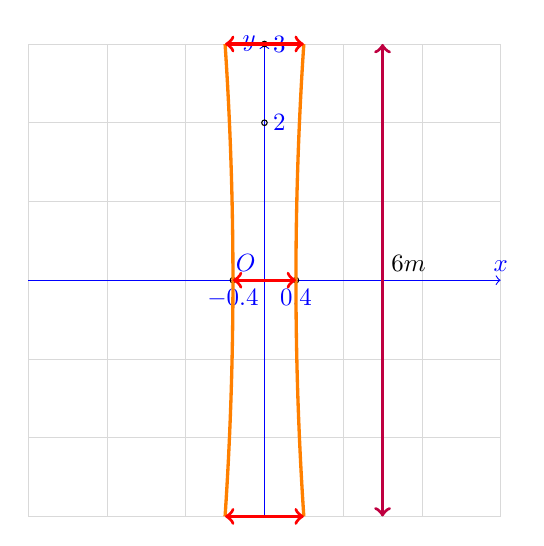
\begin{tikzpicture}[scale=1]
			\draw[step=1,gray, very thin,opacity=0.3](-3,-3) grid (3,3);
			\draw [->,blue] (-3,0) -- (3,0) node[above] {$x$};
			\draw [->,blue] (0,-3) -- (0,3) node[left] {$y$};
			\foreach \x in {-0.4,0.4} {\draw (\x,0) node[below,blue] {$\x$} circle (1pt);}
			\foreach \y in {2,3} {\draw (0,\y) node[right,blue] {$\y$} circle (1pt);}
			\draw (0,0) node [above left,blue]{$O$};
			\draw[smooth,orange, very thick] plot[domain=-3:3] ({(1/90)*(\x)^2+(2/5)}, \x);
			\draw[smooth,orange, very thick] plot[domain=-3:3] ({(-1/90)*(\x)^2-(2/5)}, \x);
			\draw[<->,red,very thick] (-0.4,0) -- (0.4,0);
			\draw[<->,red,very thick] (-0.5,3) -- (0.5,3);
			\draw[<->,red,very thick] (-0.5,-3) -- (0.5,-3);
			\draw[<->,purple,very thick] (1.5,-3) -- (1.5,3);
			\draw (1.5,0) node[above right] {$6 \text{m}$};
			\end{tikzpicture}\]
\loigiai{
Gắn hệ trục tọa độ $Oxy$ vào cột trụ hình Hypebol đã cho như hình trên.\\
Tiếp theo ta tìm phương trình của cột trụ hình Hypebol này.\\
Gọi phương trình của cột trụ là
$$\dfrac{x^{2}}{a^{2}}-\dfrac{y^{2}}{b^{2}}=1$$
Vì $Oy$ là đường trung trực của đoạn thẳng $0,8$ m nên $Oy$ chia đoạn thẳng $0,8$ m thành hai đoạn bằng nhau, mỗi đoạn $0,4$ m, tức Hypebol đi qua hai điểm $A_1(-0,4;0), A_2(0,4;0)$.\\
Khi đó ta có 
$$\dfrac{{0{,}4}^{2}}{a^{2}}-\dfrac{0^{2}}{b^{2}}=1$$
$$\Leftrightarrow \dfrac{{0{,}4}^{2}}{a^{2}}=1$$
$$\Leftrightarrow a=0{,}4.$$
(vì $a>0$)\\
Lúc này ta được phương trình Hypebol: $$\dfrac{x^{2}}{0{,}16}-\dfrac{y^{2}}{b^{2}}=1$$
Vì $Oy$ là đường trung trực của đoạn thẳng $1$ m nên $Oy$ chia đoạn thẳng $1$ m thành hai đoạn bằng nhau, mỗi đoạn $0,5$ m, tức Hypebol đi qua hai điểm $B_1(-0,5;3), B_2(0,5;3)$.\\
Khi đó ta có
$$\dfrac{{0{,}5}^{2}}{0{,}16}-\dfrac{3^{2}}{b^{2}}=1$$
$$\Leftrightarrow \dfrac{3^{2}}{b^{2}}=\dfrac{9}{16}$$
$$\Leftrightarrow b=4.$$
(vì $b>0$)\\
Vậy ta đã tìm được phương trình Hypebol của cột trụ:
$$\dfrac{x^{2}}{0{,}16}-\dfrac{y^{2}}{16}=1$$
Khi cột trụ ở độ cao $5$ m thì
$$\dfrac{x^{2}}{0{,}16}-\dfrac{5^{2}}{16}=1$$
$$\Leftrightarrow \dfrac{x^{2}}{0{,}16}=\dfrac{41}{16}$$
$$\Leftrightarrow x^{2}=\dfrac{41}{100}$$
$$\Leftrightarrow |x|=\dfrac{\sqrt{41}}{10}$$
Vậy độ rộng của cột ở độ cao $5$ m là $2.|x|=2.\dfrac{\sqrt{41}}{10}=\dfrac{\sqrt{41}}{5} \approx 1,28 \;$ m.
}
\end{bt}

% từ: cau-hoi/lop11/1D1_Ham_so_luong_giac_va_phuong_trinh_luong/1D1-1-3_So_do_cua_mot_goc_luong_giac.tex
\begin{ex}%[1D1B1-3]%[ma:129d079a]
	Hàm số  lượng giác nào dưới đây là hàm số chẵn?
	 \choice
		{$y=\sin  2x$}
		{\True $y=\cos  3x$}
		{$y=\cot  3x $}
		{$y=\tan 2x  $}
	 \loigiai{
	\begin{itemize}
		\item Hàm số $y=f(x)=\cos 3x$  là hàm số chẵn.\\
		Thật vậy, tập  xác định của nó là $\mathscr{D}=\mathbb{R}$.\\
		Với mọi $x\in \mathscr{D}$ thì $-x\in\mathscr{D}$; $f(-x)=\cos(-3x)=\cos  3x=f(x)$.
		\item Các hàm số $y=\sin2x$, $y=\cot  3x$, $y=\tan 2x$ là các hàm số lẻ.
	\end{itemize}
	 }
\end{ex}

% từ: cau-hoi/lop11/1D1_Ham_so_luong_giac_va_phuong_trinh_luong/1D1-2-3_Bien_doi_rut_gon_bieu_thuc_luong_giac_chung_m.tex
\begin{ex}%[1D1N2-3]%[ma:349c267a]
	Tính $ L=\tan20^\circ \cdot  \tan45^\circ\cdot \tan70^\circ$.
	\choice 
		 {$ 0$}
		{\True $  1$}
		{$-1$} 
		{$ 2$} 
	 \loigiai{ Ta có
		\allowdisplaybreaks\begin{eqnarray*}
		L&=&\tan20^\circ \cdot \tan45^\circ\cdot  \tan70^\circ\\
		&=& \left(\tan 20^\circ\tan 70^\circ\right)\tan 45^\circ\\ 
		 &=& \left(\tan 20^\circ \cot 20^\circ \right)\tan 45^\circ\\
		 &=&1.
\end{eqnarray*}}
\end{ex}

% từ: cau-hoi/lop11/1D1_Ham_so_luong_giac_va_phuong_trinh_luong/1D1-2-3_Bien_doi_rut_gon_bieu_thuc_luong_giac_chung_m.tex
\begin{ex}%[1D1H2-3]%[ma:16d24767]
	Không dùng máy  tính cầm tay. Hãy tính các giá trị lượng giác sau:
	\begin{listEX}[2]
		\item  $\cos 795^{\circ}$
		\item  $\tan \dfrac{7\pi}{12}$
	\end{listEX}
	\loigiai{ 
		\begin{listEX}
			\item Tính $\cos  795^\circ$.\\
			Vì $795^\circ = 75^\circ + 2 \cdot 360^\circ = 30^\circ + 45^\circ + 2 \cdot 360^\circ$ nên\\ 
			 $\cos 795^\circ = \cos 75^\circ = \cos (30^\circ + 45^\circ) = \cos 30^\circ \cos 45^\circ - \sin 30^\circ \sin 45^\circ = \dfrac{\sqrt{6}-\sqrt{2}}{4}$.
			\item Tính $\tan  \dfrac{7\pi}{12}$.\\
			$\tan \dfrac{7\pi}{12} = \tan \left(\dfrac{\pi}{3} + \dfrac{\pi}{4}\right) = \dfrac{\tan \dfrac{\pi}{3} + \tan \dfrac{\pi}{4}}{1 -  \tan \dfrac{\pi}{3} \tan \dfrac{\pi}{4}} = \dfrac{\sqrt{3} + 1}{1 - \sqrt{3}} = -2 - \sqrt{3}$.\\
		\end{listEX}
	 }
\end{ex}

% từ: cau-hoi/lop11/1D1_Ham_so_luong_giac_va_phuong_trinh_luong/1D1-2-3_Bien_doi_rut_gon_bieu_thuc_luong_giac_chung_m.tex
\begin{ex}%[1D1H2-3]%[ma:0198a1d3]
	Chứng minh các đẳng thức  sau không phụ thuộc vào biến $x$
	\begin{enumerate}
		 \item $A=-\sin ^4x+\cos ^4x+2\sin ^2x$.
		 \item $B=\sin ^4x+\cos ^2x\sin ^2x+\cos ^2x$.
		\item $B=\cos ^4x+\cos ^2x\sin ^2x+\sin  ^2x$.
	\end{enumerate}
	 \loigiai{
		\begin{enumerate}
			\item Ta có $\begin{aligned}
			-\sin ^4x+\cos ^4x+2\sin ^2x&=\left(\sin ^2x-\cos ^2x\right)\left(\sin ^2x+\cos ^2x\right)+2\sin ^2x\\ 
			 &=\sin ^2x+\cos ^2x=1.
		\end{aligned}$
		\item Ta có $\begin{aligned}
		B=&\sin ^4x+\cos ^2x\sin  ^2x+\cos ^2x=\sin ^2x\left(\sin ^2x+\cos ^2x\right)+\cos ^2x\\
		=&\sin ^2x+\cos ^2x=1. 
	\end{aligned}$
	\item Ta có $B=\cos ^4x+\cos ^2x\sin ^2x+\sin ^2x=\cos ^2x\left(\cos ^2x+\sin  ^2x\right)+\sin ^2x =\cos ^2x + \sin ^2x=1$.
	\end{enumerate}
} 
\end{ex}

% từ: cau-hoi/lop11/1D1_Ham_so_luong_giac_va_phuong_trinh_luong/1D1-2-3_Bien_doi_rut_gon_bieu_thuc_luong_giac_chung_m.tex
\begin{bt}%[1D1V2-3]%[ma:aee75aad]
% nguon: Archive/2024/SP-K10-K11-LyVanHoang_TVN-023/11. C1-LuongGiac-lvhoang_TVN-023/dataC1K11/Bai-1-Dang-8-RutGonBieuThucLuongGiac.tex #1826

	Tính giá trị biểu thức $A=\dfrac{\sin^2 a+2\sin a\cos a-2\cos^2 a}{2\sin^2 a-3\sin a\cos a+4\cos^2 a}$ khi $\cot a=-3$.
	\loigiai{
		Vì $\cot a=-3$ nên $\sin a\neq 0$. Chia cả tử và mẫu của $A$ cho $\sin a$, ta có 
		$$D=\dfrac{1+2\cot a-2\cot^2 a}{2-3\cot a+4\cot^2 a}=-\dfrac{23}{47}.$$
	}
\end{bt}

% từ: cau-hoi/lop11/1D1_Ham_so_luong_giac_va_phuong_trinh_luong/1D1-3-2_Ap_dung_cong_thuc_cong.tex
\begin{bt}%[1D1H3-2]%[ma:c571a3fd]
% nguon: Archive/SP_KhoLatex/ID6_old/1.3.1.tex #3104
%::Cau 1::
	
	Không dùng máy tính cầm tay, tính các giá trị lượng giác của các góc
	\begin{multicols}{2}
		\begin{enumerate}[a)]
		\item  $\dfrac{7\pi }{12}$;
		\item $-195^{\circ}  $.
		\end{enumerate}
	\end{multicols}
	\loigiai{
		\begin{enumerate}[a)]
		\item Ta có
		\begin{itemize}
			\item $\sin \dfrac{7\pi }{12}=\sin \left( \dfrac{\pi }{3}+\dfrac{\pi }{4} \right)=\sin \dfrac{\pi }{3}\cdot \cos \dfrac{\pi }{4}+\cos \dfrac{\pi }{3}\sin \dfrac{\pi }{4}=\dfrac{\sqrt{6}+\sqrt{2}}{4}$.\\
			\item $\cos \dfrac{7\pi }{12}=\cos \left( \dfrac{\pi }{3}+\dfrac{\pi }{4} \right)=\cos \dfrac{\pi }{3}\cdot\cos \dfrac{\pi }{4}-\sin \dfrac{\pi }{3}\sin \dfrac{\pi }{4}=\dfrac{\sqrt{2}-\sqrt{6}}{4}$.\\
			\item $\tan \dfrac{7\pi }{12}=\dfrac{\sqrt{2}+\sqrt{6}}{\sqrt{2}-\sqrt{6}}=-2-\sqrt{3}$.\\
		\end{itemize}
		\item  Ta có
		\begin{itemize}
			\item $\sin \left( -195^{\circ}  \right)=-\sin \left( 180^{\circ}  +15^{\circ}  \right)=\sin 15^{\circ}  =\sin \left( 45^{\circ}  -30^{\circ}  \right)=\dfrac{\sqrt{6}-\sqrt{2}}{4}$.\\
			\item $\cos \left( -195^{\circ}  \right)=\cos 195^{\circ}  =\cos \left( 180^{\circ}  +15^{\circ}  \right)=-\cos 15^{\circ}  =-\cos \left( 45^{\circ}  -30^{\circ}  \right)=\dfrac{\sqrt{6}+\sqrt{2}}{4}$.\\
			\item $\tan \left( -195^{\circ}  \right)=-2+\sqrt{3}.$
		\end{itemize}
	\end{enumerate}
	}
\end{bt}

% từ: cau-hoi/lop11/1D1_Ham_so_luong_giac_va_phuong_trinh_luong/1D1-3-3_Ap_dung_cong_thuc_nhan_doi_ha_bac.tex
\begin{ex}%[1D1H3-3]%[ma:f02f675a]
	Biết $\cos 2\alpha=\dfrac{5}{9}$, $0^\circ < \alpha < 90^\circ$. Khi đó 
	\choiceTF 
		{\True  $\sin\alpha=\dfrac{\sqrt{28}}{9}$}
		{\True  $\cos\alpha=\dfrac{\sqrt{53}}{9}$}
		{$\tan\alpha=\dfrac{\sqrt{371}}{53}$} 
		 {\True $\cot\alpha=\dfrac{\sqrt{371}}{14}$}
	 \loigiai{
		\begin{itemchoice}
			 \itemch \textbf{Đúng.} \\
			$\sin ^2\alpha=\dfrac{1-\cos  2\alpha}{2}=\dfrac{1-\left(\dfrac{5}{9}\right)^2}{2}=\dfrac{28}{81}\Rightarrow\sin\alpha=\pm\dfrac{\sqrt{28}}{9}$.\\
			Vì $0^\circ < \alpha <  90^\circ$ nên $\sin\alpha=\dfrac{\sqrt{28}}{9}$.
			 \itemch \textbf{Đúng.} \\
			$\cos ^2\alpha=1-\sin  ^2\alpha=1-\left(\dfrac{\sqrt{28}}{9}\right)^2=\dfrac{53}{81}\Rightarrow\cos\alpha=\pm\dfrac{\sqrt{53}}{81}$.\\
			Vì $0^\circ <  \alpha < 90^\circ$ nên $\cos\alpha=\dfrac{\sqrt{53}}{9}$.
			\itemch  \textbf{Sai.} \\
			$\tan\alpha=\dfrac{\sin\alpha}{\cos\alpha}=\dfrac{2\sqrt{371}}{53}$. 
			\itemch \textbf{Đúng.}  \\
			$\cot\alpha=\dfrac{1}{\tan\alpha}=\dfrac{\sqrt{371}}{14}$. 
		\end{itemchoice}
	} 
\end{ex}

% từ: cau-hoi/lop11/1D1_Ham_so_luong_giac_va_phuong_trinh_luong/1D1-3-3_Ap_dung_cong_thuc_nhan_doi_ha_bac.tex
\begin{bt}%[1D1H3-3]%[ma:161266ba]
% nguon: Archive/SP_KhoLatex/ID6_old/1K1-2-2.tex #3362
%[DCHT Toán 11 - KNTT -Nguyễn Thành Nhân]
Cho $\cos 2x=\dfrac{1}{3}$ Tính giá trị các biểu thức sau
\begin{listEX}[2]
\item $A=\sin^2x\cdot\cos^2x$.
\item $B=\dfrac{1+\sin^2x}{\cos^2x}$.
\item $C=\dfrac{1+\cot^2x}{1-\cot^2x}$.
\item $D=\sin^6x+\cos^6x$.
\end{listEX}
\loigiai{
\begin{enumerate}
\item $A=\dfrac{1}{2}\left(1-\cos 2x\right)\cdot\dfrac{1}{2}\left(1+\cos 2x\right)=\dfrac{1}{4}\left(1-\cos^22x\right)=\dfrac{1}{4}\left(1-\dfrac{1}{9}\right)=\dfrac{2}{9}$.
\item $B=\dfrac{1+\dfrac{1}{2}\left(1-\cos 2x\right)}{\dfrac{1}{2}\left(1+\cos 2x\right)}=\dfrac{3-\cos 2x}{1+\cos 2x}=\dfrac{3-\dfrac{1}{3}}{1+\dfrac{1}{3}}=2$.
\item $C=\dfrac{\sin^2x+\cos^2x}{\sin^2x-\cos^2x}=\dfrac{-1}{\cos 2x}=\dfrac{-1}{\dfrac{1}{3}}=-3$.
\item \begin{eqnarray*}
D&=&\left(\sin^2x+\cos^2x\right)^3-3\sin^2x\cos^2x\left(\sin^2x+\cos^2x\right)\\
&=&1-\dfrac{3}{4}\left(1-\cos^22x\right)=\dfrac{1}{4}+\dfrac{3}{4}\cos^22x\\
&=& \dfrac{1}{4}+\dfrac{3}{4}\cdot \dfrac{1}{9}=\dfrac{1}{3}.
\end{eqnarray*}
\end{enumerate}
}
\end{bt}

% từ: cau-hoi/lop11/1D1_Ham_so_luong_giac_va_phuong_trinh_luong/1D1-3-3_Ap_dung_cong_thuc_nhan_doi_ha_bac.tex
\begin{bt}%[1D1H3-3]%[ma:2e0704b2]
% nguon: Archive/SP_KhoLatex/ID6_old/1K1-2.tex #3588
%[Dự án 1 - TLDH - TeamTeXHoa - Huỳnh Xuân Tín]
	Cho $\cos 4 \alpha+2=6 \sin ^2 \alpha$ với $\dfrac{\pi}{2}<\alpha<\pi$. Tính tan $2 \alpha$.
	\loigiai{
		Ta có $\cos 4 \alpha+2=6 \sin ^2 \alpha \Leftrightarrow 2 \cos ^2 2 \alpha-1+2=3(1-\cos 2 \alpha)$\\
		$\Leftrightarrow 2 \cos ^2 2 \alpha+3 \cos 2 \alpha-2=0 \Leftrightarrow \cos 2 \alpha=\dfrac{1}{2}$.\\
		Ta có $1+\tan ^2 2 \alpha=\dfrac{1}{\cos ^2 2 \alpha} \Rightarrow \tan ^2 2 \alpha=\dfrac{1}{\cos ^2 2 \alpha}-1=3$.\\
		Vì $\dfrac{\pi}{2}<\alpha<\pi \Rightarrow \pi<\alpha<2 \pi$ nên $\sin 2 \alpha<0$. Mặt khác $\cos 2 \alpha>0$ do đó $\tan 2 \alpha<0$.\\
		Vậy $\tan 2 \alpha=-\sqrt{3}$.
	}	
\end{bt}

% từ: cau-hoi/lop11/1D1_Ham_so_luong_giac_va_phuong_trinh_luong/1D1-3-3_Ap_dung_cong_thuc_nhan_doi_ha_bac.tex
\begin{ex}%[1D1H3-3]%[ma:35d4a71a]
	Cho $\sin \alpha =\dfrac{1}{2}$.  Giá trị của $P=\cos 2\alpha+\sin \alpha$ bằng
	 \choice
		{\True  $1$}
		{$2$} 
		 {$\dfrac{1}{2}$}
		{$0$} 
	\loigiai{Ta  có \allowdisplaybreaks
		\begin{eqnarray*}
			 P&=&\cos 2\alpha +3\sin \alpha\\
			 &=&1-2\sin^2 \alpha+\sin \alpha \\
			&=&1-2\left(\dfrac{1}{2}\right)^2+\dfrac{1}{2}=1. 
		\end{eqnarray*}
	 }
\end{ex}

% từ: cau-hoi/lop11/1D1_Ham_so_luong_giac_va_phuong_trinh_luong/1D1-3-4_Ap_dung_cong_thuc_bien_doi_tich_tong.tex
\begin{bt}%[1D1H3-4]%[ma:0a505467]
% nguon: Archive/2024/TOAN_11_XE/TOAN_11_XE/data4/11C1/KNTT-1.2.tex #1146
%%[DCHT Toán 11 - KNTT -Nguyễn Thành Nhân]
	Rút gọn các biểu thức sau
	\begin{listEX}[2]
		\item $A=\cos 11x\cos 3x-\cos 17x\cos 9x$.
		\item $B=\sin 18x\cos 3x-\sin 19x\cos 4x$.
		\item $C=\sin x\sin 3x+\sin 4x\sin 8x$.
		\item $D=\sin 2x\sin 6x-\cos x\cos 3x$.
	\end{listEX}
	\loigiai{
		\begin{enumerate}
			\item $A=\dfrac{1}{2}\cos 14x+\dfrac{1}{2}\cos 8x-\dfrac{1}{2}\cos 26x-\dfrac{1}{2}\cos 8x=\dfrac{1}{2}\left(\cos 14x-\cos 26x\right)=\sin 15x\sin 12x$.
			\item $B=\dfrac{1}{2}\sin 21x+\dfrac{1}{2}\sin 15x-\dfrac{1}{2}\sin 23x-\dfrac{1}{2}\sin 15x=\dfrac{1}{2}\left(\sin 21x-\sin 23x\right)=-\cos 22x\sin x$.
			\item $C=-\dfrac{1}{2}\cos 4x+\dfrac{1}{2}\cos 2x-\dfrac{1}{2}\cos 12x+\dfrac{1}{2}\cos 4x=\dfrac{1}{2}\left(\cos 12x+\cos 2x\right)=\cos 7x\cos 5x$.
			\item $D=-\dfrac{1}{2}\cos 8x+\dfrac{1}{2}\cos 4x-\dfrac{1}{2}\cos 4x-\dfrac{1}{2}\cos 2x=-\dfrac{1}{2}\left(\cos 8x+\cos 2x\right)=-\cos 5x\cos 3x$.
		\end{enumerate}
	}
\end{bt}

% từ: cau-hoi/lop11/1D1_Ham_so_luong_giac_va_phuong_trinh_luong/1D1-3-5_Ket_hop_nhieu_cong_thuc_luong_giac.tex
\begin{ex}%[1D1H3-5]%[ma:9fe42cb6]
	Biết  $\sin\alpha=\dfrac{1}{3}$ và $ 0 <\alpha <\dfrac{\pi}{2}$. Khi đó
	 \choiceTF
		{$\sin 2\alpha=\dfrac{\sqrt  2}{9}$}
		{\True $\cos  2\alpha=\dfrac{7}{9}$}
		{$\tan 2\alpha=\dfrac{\sqrt  2}{7}$}
		{$\cot 2\alpha=\dfrac{7\sqrt 2}{2}$} 
	\loigiai{ 
		Ta có $\cos  ^2\alpha+\sin ^2\alpha =1 \Rightarrow \cos ^2\alpha=1-\sin ^2\alpha=1-\left(\dfrac{1}{3}\right)^2=\dfrac{8}{9}\Rightarrow\cos\alpha=\pm\dfrac{2\sqrt 2}{3}$.\\
		Vì $ 0 <\alpha  <\dfrac{\pi}{2}$ nên $\cos\alpha=\dfrac{2\sqrt 2}{3}$. Khi đó
		\begin{itemize}
			\item  $\sin 2\alpha=2\sin\alpha\cdot\cos\alpha=2\cdot\dfrac{1}{3}\cdot\dfrac{2\sqrt 2}{3}=\dfrac{4\sqrt 2}{9}$.
			\item  $\cos 2\alpha=\cos ^2\alpha-\sin ^2\alpha=\left(\dfrac{2\sqrt 2}{3}\right)^2-\left(\dfrac{1}{3}\right)^2=\dfrac{7}{9}$.
			\item $\tan 2\alpha=\dfrac{\sin 2\alpha}{\cos 2\alpha}=\dfrac{4\sqrt 2}{2}:\dfrac{7}{9}=\dfrac{4\sqrt  2}{7}$.
			\item $\cot 2\alpha=\dfrac{\cos 2\alpha}{\sin 2\alpha}=\dfrac{4\sqrt  2}{2}:\dfrac{7}{9}=\dfrac{7\sqrt 2}{8}$.
		\end{itemize}
	 }
\end{ex}

% từ: cau-hoi/lop11/1D1_Ham_so_luong_giac_va_phuong_trinh_luong/1D1-4-3_Xet_tinh_don_dieu.tex
\begin{ex}%[1D1H4-3]%[ma:58824536]
	Cho các hàm số sau $f(x)=\sin  x$ và $g(x)=\cos x$. Khi đó
	 \choiceTF{\True Hàm số $f(x)=\sin x$ đồng biến trên khoảng $\left(-\dfrac{\pi}{2}; \dfrac{\pi}{2}\right)$}
		{\True Hàm số $f(x)$ nghịch biến trên khoảng  $\left(\dfrac{3\pi}{4}; \dfrac{5\pi}{4}\right)$}
		{\True Hàm số  $g(x)$ nghịch biến trên khoảng $(0; \pi)$}
		{Hàm số $g(x)$  đồng biến trên khoảng $\left(\dfrac{25\pi}{6}; \dfrac{13\pi}{3}\right)$}
	 \loigiai{
		\begin{itemchoice}
			 \itemch \textbf{Đúng.}\\
			Hàm số $f(x)=\sin x$ đồng biến trên khoảng  $\left(-\dfrac{\pi}{2}; \dfrac{\pi}{2}\right)$.
			\itemch  \textbf{Đúng.}\\
			Vì $\left(\dfrac{3\pi}{4}; \dfrac{5\pi}{4}\right)\subset \left(\dfrac{\pi}{2}; \dfrac{3\pi}{2}\right)$ nên hàm số $f(x)$ nghịch biến trên  khoảng $\left(\dfrac{3\pi}{4}; \dfrac{5\pi}{4}\right)$.
			\itemch  \textbf{Đúng.}\\
			Hàm số $g(x)=\cos x$ nghịch biến trên khoảng  $(0; \pi)$.
			 \itemch \textbf{Sai.}\\
			Vì $\dfrac{25\pi}{6}=\dfrac{\pi}{6}+4\pi, \dfrac{13\pi}{3}=\dfrac{\pi}{3}+4\pi$, đồng thời $\left(\dfrac{\pi}{6}; \dfrac{\pi}{3}\right)\subset \left(0; \dfrac{\pi}{2}\right)$ nên hàm số $g(x)=\cos x$ nghịch biến trên khoảng $\left(\dfrac{\pi}{6}; \dfrac{\pi}{3}\right)$, suy ra hàm số cũng nghịch biến trên khoảng  $\left(\dfrac{25\pi}{6}; \dfrac{13\pi}{3}\right)$.
		\end{itemchoice}
	 }
\end{ex}

% từ: cau-hoi/lop11/1D1_Ham_so_luong_giac_va_phuong_trinh_luong/1D1-4-6_Tim_tap_gia_tri_va_min_max.tex
\begin{ex}%[1D1H4-6]%[ma:b972812e]
	Tìm giá trị lớn nhất, giá trị nhỏ nhất của hàm số sau đây: 
	\begin{enumEX}{2}
		\item $y=2\sin\left(x+\dfrac{\pi}{4}\right)+1$; 
		\item $y=2\sqrt{\cos  x+1}-3$;
		 \item $y=\sin x+\cos x$;
		\item $y=\sqrt{3}\sin  2x-\cos 2x$;
		\item $y=\cos^2x+2\sin x+2$; 
		 \item $y=\sin^4x-2\cos^2x+1$.
	\end{enumEX}
	\loigiai{ 
		\begin{enumerate}
			 \item Ta có \allowdisplaybreaks
			\begin{eqnarray*}
				&&-1 \leq  \sin\left(x+\dfrac{\pi}{4}\right) \leq 1 \\
				 &\Rightarrow& -2 \leq 2\sin\left(x+\dfrac{\pi}{4}\right) \leq 2 \\
				&\Rightarrow& -1 \leq  2\sin\left(x+\dfrac{\pi}{4}\right)+1 \leq 3\\
				&\Rightarrow&-1 \leq  y \leq 3.
			\end{eqnarray*}
			\begin{itemize}
				\item $\max y=3$ khi  $\sin\left(x+\dfrac{\pi}{4}\right)=1\Leftrightarrow x=\dfrac{\pi}{4}+k2\pi,\, k\in\mathbb{Z}$.
				\item $\min y=-1$ khi $\sin\left(x+\dfrac{\pi}{4}\right)=-1\Leftrightarrow x=-\dfrac{3\pi}{4}+k2\pi,\,  k\in\mathbb{Z}$.
			\end{itemize}
			 \item Ta có\allowdisplaybreaks
			\begin{eqnarray*}
				&&-1 \leq \cos x \leq 1 \\ 
				&\Rightarrow& 0 \leq  \cos x+1 \leq 2 \\
				&\Rightarrow& 0  \leq \sqrt{\cos x+1} \leq \sqrt{2}\\
				&\Rightarrow& 0 \leq 2\sqrt{\cos x+1} \leq 2\sqrt{2}\\  &\Rightarrow& -3 \leq 2\sqrt{\cos x+1}-3 \leq 2\sqrt{2}-3\\
				&\Rightarrow&-3 \leq y  \leq 2\sqrt{2}-3.
			\end{eqnarray*}
			\begin{itemize}
				\item $\max y=2\sqrt{2}-3$ khi  $\cos x=1\Leftrightarrow x=k2\pi,\,k\in\mathbb{Z}$.
				\item  $\min y=-3$ khi $\cos x=-1\Leftrightarrow x=\pi+k2\pi,\,k\in\mathbb{Z}$.
			\end{itemize}
			\item Ta  có $y=\sin x+\cos x=\sqrt{2}\sin\left(x+\dfrac{\pi}{4}\right)\Rightarrow-\sqrt{2}\leq y\leq\sqrt{2}$.
			\begin{itemize}
				\item $\max y=\sqrt{2}$ khi $\sin\left(x+\dfrac{\pi}{4}\right)=1\Leftrightarrow x=\dfrac{\pi}{4}+k2\pi,\,k\in\mathbb{Z}$. 
				\item  $\min y=-\sqrt{2}$ khi $\sin\left(x+\dfrac{\pi}{4}\right)=-1\Leftrightarrow x=-\dfrac{3\pi}{4}+k2\pi,\,k\in\mathbb{Z}$.
			\end{itemize}
			\item Ta  có $y=\sqrt{3}\sin 2x-\cos 2x=2\left(\dfrac{\sqrt{3}}{2}\sin 2x-\dfrac{1}{2}\cos 2x\right)=2\sin\left(2x-\dfrac{\pi}{6}\right)\Rightarrow-2\leq y\leq 2$.
			\begin{itemize}
				\item $\max y=2$ khi $\sin\left(2x-\dfrac{\pi}{6}\right)=1\Leftrightarrow 2x-\dfrac{\pi}{6}=\dfrac{\pi}{2}+k2\pi\Leftrightarrow x=\dfrac{\pi}{3}+k\pi,  k\in\mathbb{Z}$.
				\item $\min y=-2$  khi $\sin\left(2x-\dfrac{\pi}{6}\right)=-1\Leftrightarrow 2x-\dfrac{\pi}{6}=-\dfrac{\pi}{2}+k2\pi\Leftrightarrow x=-\dfrac{\pi}{6}+k\pi, k\in\mathbb{Z}$.
			\end{itemize}
			\item Ta có 
			$y=\cos^2x+2\sin x+2=(1-\sin^2x)+2\sin x+2=-\sin^2x+2\sin x+3=-(\sin x-1)^2+4$.\\ 
			Vì  \allowdisplaybreaks
			\begin{eqnarray*}
				&&-1 \leq \sin x  \leq 1\\
				& \Rightarrow& -2 \leq \sin  x - 1 \leq 0 \\
				&\Rightarrow& 4 \geq (\sin x - 1)^2 \geq  0\\
				 &\Rightarrow &-4 \leq -(\sin x - 1)^2 \leq 0 \\
				&\Rightarrow& 0 \leq -(\sin x  - 1)^2 + 4 \leq 4 \\
				&\Rightarrow& 0 \leq y \leq  4.
			\end{eqnarray*}
			\begin{itemize}
				\item $\max y=4$ khi $\sin  x=1\Leftrightarrow x=\dfrac{\pi}{2}+k2\pi,\,k\in\mathbb{Z}$.
				 \item $\min y=0$ khi $\sin x=-1\Leftrightarrow x=-\dfrac{\pi}{2}+k2\pi,\,k\in\mathbb{Z}$.
			\end{itemize}
			 \item Ta có \allowdisplaybreaks
			\begin{eqnarray*}
				y& =& \sin^4 x - 2\cos^2  x + 1 \\
				&=& (1-\cos^2 x)^2 - 2\cos^2  x + 1\\
				& =& \cos^4 x - 4\cos^2 x + 2  \\
				&=& (\cos^2  x - 2)^2 - 2.
			\end{eqnarray*}
			 Ta có
			\allowdisplaybreaks 
			\begin{eqnarray*}
				&&0 \leq \cos^2 x \leq  1 \\
				&\Rightarrow& -2 \leq \cos^2 x - 2 \leq -1  \\
				&\Rightarrow& 4 \geq (\cos^2 x - 2)^2  \geq 1\\
				&\Rightarrow& 2 \geq (\cos^2 x - 2)^2 -  2 \geq -1 \\
				&\Rightarrow&  -1 \leq y \leq 2.
			\end{eqnarray*}
			\begin{itemize}
				\item $\max y=2$ khi $\cos^2x=0\Leftrightarrow\cos x=0\Leftrightarrow  x=\dfrac{\pi}{2}+k\pi,\,k\in\mathbb{Z}$.
				\item $\min y=-1$ khi $\cos^2x=1\Leftrightarrow\sin x=0\Leftrightarrow  x=k\pi,\, k\in\mathbb{Z}$.
			\end{itemize}
		\end{enumerate}
	} 
\end{ex}

% từ: cau-hoi/lop11/1D1_Ham_so_luong_giac_va_phuong_trinh_luong/1D1-4-8_Toan_thuc_te_ap_dung_ham_so_luong_giac.tex
\begin{bt}%[1D1V4-8]%[ma:5039b4ae]
% nguon: Archive/2024/SP-K10-K11-LyVanHoang_TVN-023/11. C1-LuongGiac-lvhoang_TVN-023/dataC1K11/Bai-3-Dang-6-Dothihamsoluonggiac.tex #2070
%[BG K11, Nhật Thiện]
	[Mức độ 3]
	\immini{
		Khi đu quay hoạt động, vận tốc theo phương ngang của một cabin $M$ phụ thuộc vào góc lượng giác $\alpha = \left(Ox,OM\right)$ theo hàm số $v_x = 0{,}3\sin\alpha$ (m/s) (Hình vẽ bên). Dựa vào đồ thị của hàm số sin, biết trong vòng quay đầu tiên $\left(0\le \alpha\le 2\pi\right)$, góc $\alpha$ ở trong các khoảng $\left(0;\dfrac{\pi}{a}\right)$ và $\left(\dfrac{b\pi}{2};2\pi\right)$ thì $v_x$ tăng. Biết $a$, $b\in \mathbb{Z}$, tính $a+b$.
	}{\begin{tikzpicture}[scale=0.5,font=\small,line join=round,line cap=round,>=stealth]
		\tikzset{declare function={g=0;}}
		\coordinate (O) at (0,0);
		\coordinate[label=above right:$A$] (A) at (0:4.4);
		\coordinate[label=above right:$M$] (M) at (30+g:4.4);
		\pgfmathsetmacro{\gx}{60-g};
		\coordinate (v) at ($(M)+(120+g:3.3)$);
		\coordinate (vx) at ($(M)+(180:3.3*cos \gx)$);
		\draw[thick] (O) circle(4.4) (O) circle(3.53);
		\foreach \t in {0,1,...,11}{
			\draw[very thick,fill] (O)--(g+30*\t:4.4)circle(0.06);
			\begin{scope}[shift={(g+30*\t:4.4)}]
				\draw[fill=teal] (-0.27,0)--(0.27,0)--(0.36,-0.18)--(-0.36,-0.18)--cycle
				(0.32,-0.18)--(0.32,-0.54) (-0.32,-0.18)--(-0.32,-0.54)
				(-0.4,-0.54)--(0.4,-0.54)--(0.27,-1)--(-0.27,-1)--cycle;
		\end{scope}}
		\draw[fill=gray!70!yellow] (0.2,0)--(2.35,-5.53)--(3.65,-5.53)--(3.65,-6.02)--(1.95,-6.02)--(0,-0.85)--(-1.95,-6.02)--(-3.65,-6.02)--(-3.65,-5.53)--(-2.35,-5.53)--(-0.2,0)--cycle;
		\draw[fill=gray!10!yellow] (O) circle(0.34);
		\draw[fill] (-5,-5.85)--(0,-5.85) circle(0.08)--(6.4,-5.85);
		\draw[->,red] (-5,0)--(6.7,0) node [below]{\color{black}$x$};
		\draw[->,red] (M)--(v) node [left=-2pt]{\color{black}$\overrightarrow{v}$};
		\draw[->,red] (M)--(vx) node [below left=-5pt]{\color{black}$\overrightarrow{v}_{\!\!x}$};
		\draw[red] (O)--(M);
		\draw[dashed,red] (0,0)--(0,-5.85) (v)--(vx);
		\fill (0,0) circle(0.1);
		\path pic[draw=red,angle radius=5]{right angle=v--M--O} 
		(O) pic[draw,->,angle radius=16]{angle=A--O--M} node[shift={(14:23pt)}]{$\alpha$};
		\node at (O)[below]{$O$};
	\end{tikzpicture}	
	}
	\shortans[]{$5$}
	\loigiai{
		Ta có đồ thị của hàm số $v_x$ trên $\left[0;2\pi\right]$ như sau.
			\immini{
				Dựa vào đồ thị ta có trên các khoảng $\left(0;\dfrac{\pi}{2}\right)$ và $\left(\dfrac{3\pi}{2};2\pi\right)$ thì $v_x$ tăng.\\
				Suy ra $a=2$, $b=3$.\\
				Vậy $a+b=5$.
			}{
				\begin{tikzpicture}[>=stealth,x=1.0cm,y=1.0cm, scale=1]
					\draw[->](-1,0) -- (7,0) node[below]{\footnotesize $x$};
					\draw[->](0,-1.5) -- (0,1.85) node[right]{\footnotesize $v_x$};
					\draw[fill = black] (0,0) node [above left]{$O$} circle (1pt);
					\draw[fill = black] (pi,0) node [above right]{\footnotesize $\pi$} circle (1pt);
					\draw[fill = black] (2*pi,0) node [above]{\footnotesize $2\pi$} circle (1pt);
					\draw[fill = black] (pi/2,0) node [below]{\footnotesize $\tfrac{\pi}{2}$} circle (1pt);
					\draw[fill = black] (3*pi/2,0) node [above]{\footnotesize $\tfrac{3\pi}{2}$} circle (1pt);
					\draw[smooth, samples=100, domain=0:6.3]plot(\x,{sin((\x)*180/pi)});
					\draw[dashed] (pi/2,0)--(pi/2,1)--(0,1) node[left]{\footnotesize$0{,}3$} (3*pi/2,0)--(3*pi/2,-1)--(0,-1) node[left]{\footnotesize$-0{,3}$};
				\end{tikzpicture}
			}
	}
\end{bt}

% từ: cau-hoi/lop11/1D1_Ham_so_luong_giac_va_phuong_trinh_luong/1D1-5-3_Phuong_trinh_co_ban_dung_Radian.tex
\begin{bt}%[1D1H5-3]%[ma:f9dc2cab]
% nguon: Archive/SP_DA_SauLuoi/1-TL-THPT-Marie-Curie-GHKI-NH23-24.tex #2463
%[Dự án Tex đề GHK-HK 2023-2024]%[Nhật Thiện]%[THPT Marie Curie]
    Giải các phương trình lượng giác sau
    \begin{enumEX}{2}
        \item $\cos  x=\dfrac{\sqrt{3}}{2}$;
        \item $\sin x+\cos \dfrac{\pi}{7}=0$.
    \end{enumEX}
    \loigiai{
        \begin{enumerate}
            \item Ta có  $\cos x=\dfrac{\sqrt{3}}{2}\Leftrightarrow \cos x=\cos \dfrac{\pi}{3}\Leftrightarrow \hoac{&x=\dfrac{\pi}{3}+k2\pi\\&x=-\dfrac{\pi}{3}+k2\pi}$, $k\in\mathbb{Z}$.
            \item Ta có
            \begin{eqnarray*}
                & &\sin x=-\cos \dfrac{\pi}{7}\Leftrightarrow \sin x=-\sin \left(\dfrac{5\pi}{14}\right)\Leftrightarrow \sin x=\sin \left(-\dfrac{5\pi}{14}\right)\\
                &\Leftrightarrow&  \hoac{&x=-\dfrac{5\pi}{14}+k2\pi\\&x=\pi-\dfrac{5\pi}{14}+k2\pi},\,k\in\mathbb{Z}\\
                &\Leftrightarrow& \hoac{&x=-\dfrac{5\pi}{14}+k2\pi\\&x=\dfrac{9\pi}{14}+k2\pi},\,k\in\mathbb{Z}.
            \end{eqnarray*}
        \end{enumerate}
    }
\end{bt}

% từ: cau-hoi/lop11/1D1_Ham_so_luong_giac_va_phuong_trinh_luong/1D1-5-3_Phuong_trinh_co_ban_dung_Radian.tex
\begin{bt}%[1D1H5-3]%[ma:2d482f15]
% nguon: Archive/SP_KhoLatex/ID6_old/1K1-4.tex #3795
%[Dự án 1 - TLDH - TeamTeXHoa - Nguyễn Cường]
	Giải các phương trình
	\begin{multicols}{2}
		\begin{enumerate}
			\item $\sin 3x=\dfrac{1}{2}$;
			\item $\cos 2x=-\dfrac{1}{2}$;
			\item $\tan\dfrac{x}{3}=2$;
			\item $\cot\left(2x+\dfrac{\pi}{4}\right)=\sqrt{3}$.
		\end{enumerate}
	\end{multicols}
	\loigiai 
	{
	\begin{enumerate}
		\item $\sin 3x=\dfrac{1}{2}\Leftrightarrow\hoac{&3x=\dfrac{\pi}{6}+k2\pi\\&3x=\pi-\dfrac{\pi}{6}+k2\pi}\Leftrightarrow\hoac{&x=\dfrac{\pi}{18}+\dfrac{k2\pi}{3}\\&x=\dfrac{5\pi}{18}++\dfrac{k2\pi}{3}},\,k\in\mathbb{Z}$.
		\item $\cos 2x=-\dfrac{1}{2}\Leftrightarrow\hoac{&2x=\dfrac{2\pi}{3}+k2\pi\\&2x=-\dfrac{2\pi}{3}+k2\pi}\Leftrightarrow\hoac{&x=\dfrac{\pi}{3}+k\pi\\&x=-\dfrac{\pi}{3}+k\pi},\,k\in\mathbb{Z}$;
		\item Với $\tan \alpha=2$, ta có
		$$\tan\dfrac{x}{3}=2\Leftrightarrow \tan\dfrac{x}{3}=\tan\alpha\Leftrightarrow \dfrac{x}{3}=\alpha+k\pi\Leftrightarrow x=3\alpha+k3\pi,\,k\in\mathbb{Z}.$$
		\item $\cot\left(2x+\dfrac{\pi}{4}\right)=\sqrt{3}\Leftrightarrow 2x+\dfrac{\pi}{4}=\dfrac{\pi}{6}+k\pi\Leftrightarrow x=-\dfrac{\pi}{24}+\dfrac{k\pi}{2},\,k\in\mathbb{Z}$.
	\end{enumerate}
	}
\end{bt}

% từ: cau-hoi/lop11/1D1_Ham_so_luong_giac_va_phuong_trinh_luong/1D1-5-6_Toan_thuc_te_ap_dung_phuong_trinh_luong_giac.tex
\begin{ex}%[1D1H5-6]%[ma:e40eb753]
	 \immini[thm]{
	Một vòng quay trò chơi có bán kính $57$ m, trục quay cách mặt đất $57{,}5$ m, quay đều mỗi vòng hết $15$ phút. Khi vòng quay quay đều, khoảng cách $h$ mét từ một cabin gắn tại điểm $A$ của vòng quay đến mặt  đất được tính bởi công thức
	$$ h(t)=57\sin\left(\dfrac{2\pi}{15}t-\dfrac{\pi}{2}\right)+57{,}5,$$ 
	với $t$ là thời gian  quay của vòng quay tính bằng phút $\left(t\ge 0\right)$. Khi quay một vòng lần thứ nhất tính từ thời điểm $t=0$ phút, tại thời điểm nào của $t$ thì cabin ở vị trí cao nhất?
	 }
	{ 
	\begin{tikzpicture}[scale=.6,font=\footnotesize,line join=round,
				line cap=round,>=stealth] 
			\draw (0:0) coordinate (O)--++(50:4) coordinate (A) 
				(A) arc (50:410:4) 
				(O)--++(-90:5)  coordinate (G)
				(-4.5,-5)--(4.5,-5); 
			\draw[dashed] (A)--++(-90:8.05)  coordinate (H);
			\foreach  \x/\g in {O/180,A/30}
			 \fill[black](\x) circle (2pt)
				 ($(\x)+(\g:4mm)$) node{$\x$};
			 \draw ($(A)!.5!(H)$) node[left]{$h$};
			\draw ($(A)!.5!(O)$) node[above,rotate=50]{$57$  m};
			\draw ($(O)!.5!(G)$) node[left]{$57{,}5$  m};
			\fill[black] (H)  circle (2pt);
			\fill[black] (0,-5)  circle (2pt);
		\end{tikzpicture}
	} 
	 \shortans{7,5}
	\loigiai{ 
		Khi quay  một vòng, cabin ở vị trí cao nhất khi $\sin\left(\dfrac{2\pi}{15}t-\dfrac{\pi}{2}\right)=1$ hay $t=7{,}5$ phút.
	 }
\end{ex}

% từ: cau-hoi/lop11/1D1_Ham_so_luong_giac_va_phuong_trinh_luong/1D1-6-1_Phuong_trinh_bac_n_theo_mot_ham_so_luong_giac.tex
\begin{ex}%[1D1H6-1]%[ma:b68762ed]
		 Giải phương trình $\cos 2x+2\cos x-3=0$.
	 \choice
			{$x=\pi+k2\pi,k\in\mathbb{Z}$} 
			 {\True $x=k2\pi,k\in\mathbb{Z}$}
			{$x=-\dfrac{\pi}{2}+k2\pi,k\in\mathbb{Z}$} 
			{$x=\dfrac{\pi}{2}+k2\pi,k\in\mathbb{Z}$} 
	\loigiai{ 
			$\cos 2x+2\cos x-3=0\Leftrightarrow 2\cos^2x+2\cos x-4=0\Leftrightarrow \hoac{&\cos x=1\\&  \cos x=-2\;\text{(loại)}}\Leftrightarrow x=k2\pi,k\in\mathbb{Z}$.
		 }
\end{ex}

% từ: cau-hoi/lop11/1D2_Day_so_Cap_so_cong_Cap_so_nhan/1D2-1-1_Cau_hoi_ly_thuyet.tex
\begin{ex}%[1D2Y1-1]%[ma:a3b35e9b]
	Trong các dãy số  $(u_n)$ sau, dãy số nào bị chặn dưới, bị chặn trên, bị chặn?
	\begin{enumEX}[a)]{4}
		\item  $u_n=n-1$;
		\item  $u_n=\dfrac{n+1}{n+2}$;
		\item $u_n=\sin  n$;
		\item $u_n=(-1)^{n-1} n^2$. 
	\end{enumEX}
	\loigiai{\begin{enumEX}[a)]{1}
		\item Dãy số $u_n=n-1$ bị chặn dưới, vì $u_{n}\ge 0,\, \forall n  \in \mathbb{N}^{*}$.
		 \item Dãy số $u_n=\dfrac{n+1}{n+2}$ bị chặn trên, vì $u_n=1-\dfrac{1}{n+2}<1,\, \forall n \in \mathbb{N}^{*}$.\\
		 Dãy số $\left(u_{n}\right)$ cũng bị chặn dưới, vì $u_n=\dfrac{n+1}{n+2} \geq \dfrac{2}{3},\, \forall n \in \mathbb{N}^{*}$.\\
		Vậy dãy số $\left(u_{n}\right)$  bị chặn.
		\item Dãy số $u_n=\sin  n$ bị chặn trên, bị chặn dưới, vì $-1\le \sin n \le1,\, \forall n \in \mathbb{N}^{*}$.\\
		Vậy dãy  số $\left(u_{n}\right)$ bị chặn.
		\item Bốn số hạng  đầu của dãy số là \\$u_2=(-1)^1\cdot 2^2=-4;$ $u_3=(-1)^2\cdot 3^2=9;$ $u_4=(-1)^3 \cdot 4^2=-16;$ $u_5=(-1)^4\cdot 5^2=25;$ $\cdots$
		\\ 
		Vậy dãy số  không bị chặn.
\end{enumEX}}
\end{ex}

% từ: cau-hoi/lop11/1D2_Day_so_Cap_so_cong_Cap_so_nhan/1D2-3-4_Tim_so_hang_cu_the_trong_cap_so_nhan.tex
\begin{ex}%[1D2V3-4]%[ma:089522db]
	Một tứ giác lồi có số đo các góc lập thành một cấp số nhân. Biết rằng số đo của góc nhỏ nhất bằng $\dfrac{1}{9}$ số đo của góc nhỏ thứ ba. Hãy tính số đo của các góc trong tứ  giác đó.
	 \choice
		{$5^\circ$, $ 15^\circ$, $ 45^\circ$, $  225^\circ$}
		{\True $9^\circ$, $ 27^\circ$, $  81^\circ$, $ 243^\circ$}
		{$7^\circ$, $ 21^\circ$, $ 63^\circ$, $ 269^\circ$} 
		{$8^\circ$, $ 32^\circ$, $  72^\circ$, $ 248^\circ$}
	 \loigiai{
		Gọi số đo các góc của tứ giác là $a$, $aq$, $aq^2$, $aq^3$, trong đó $q >  1$.\\
		Theo giả thiết,  ta có $a=\dfrac{1}{9} aq^2$ nên $q=3$.\\
		Suy ra các góc của tứ giác là  $a$, $3a$, $9a$, $27a$.\\
		Vì tổng các góc trong tứ  giác bằng $360^\circ$ nên ta có $a+3a+9a+27a=360^\circ \Leftrightarrow a=9^\circ$.
	} 
\end{ex}

% từ: cau-hoi/lop11/1D2_Day_so_Cap_so_cong_Cap_so_nhan/1D2-3-6_Tinh_tong_cua_cap_so_nhan.tex
\begin{ex}%[1D2V3-6]%[ma:3a4d4101]
	Cho dãy số $(u_n)$ thỏa mãn $\heva{& u_1=1 \\& u_n=2u_{n-1}+1;n \geq 2}$. Tổng $S=u_1+u_2+\dots+u_{20}$ bằng 
	 \choice
		 {$2^{20}-20$}
		 {\True $2^{21}-22$}
		 {$2^{20}$}
		 {$2^{21}-20$}
	\loigiai{Ta có $u_n = 2u_{n-1} + 1  \Leftrightarrow u_n + 1 = 2(u_{n-1} + 1)$.\\
		 Đặt $v_n = u_n + 1$, ta có $v_n = 2v_{n-1}$ trong đó $v_1 = 2$.\\
		Vậy $(v_n) $ là cấp số nhân có số hạng đầu $v_1  = 2$ và công bội bằng $2$, nên số hạng tổng quát\\
		$v_n = 2^n \Rightarrow u_n = v_n - 1 =  2^n - 1$.\\
		Vậy  nên
		\begin{align*}
			S &= u_1  + u_2 + \dots + u_{20} =(2^1 - 1) +(2^2 - 1) + \dots +(2^{20} - 1) \\&=(2^1 + 2^2 + \dots + 2^{20}) - 20 \\&= 2\cdot(2^{20} - 1) - 20 \\&= 2^{21} - 22.
		\end{align*}
	 }
\end{ex}

% từ: cau-hoi/lop11/1D3_Gioi_han_Ham_so_lien_tuc/1D3-1-2_Phuong_phap_dat_thua_so_chung_lim_huu_han.tex
\begin{bt}%[1D3V1-2]%[ma:0958f8fc]
% nguon: Archive/SP_KhoLatex/ID6_old/15-OT-GioiHan-LienTuc.tex #2681
%[DGNL-DGTD-2022]%[Huỳnh Xuân Tín]
	Tính giới hạn $L=\dfrac{5 + 9 + 13 + \dots + 4n - 3}{3n^2 + 5n - 1}$. 
	\loigiai{
		Xét cấp số cộng $5, 9, 13, \ldots, 4n-3$ có số hạng đầu $u_1=5$, công sai $d=4$ và số hạng cuối $4n-3=5+(n-2)\cdot 4=u_{n-1}$. Suy ra tổng $5+9+13+\cdots+4n-3=\dfrac{(5+4n-3)(n-1)}{2}=\dfrac{4n^2-2n-2}{2}$.\\
		Do đó $$L=\dfrac{5 + 9 + 13 + \dots + 4n - 3}{3n^2 + 5n - 1}=\lim \dfrac{4n^2-2n-2}{2(3n^2 + 5n - 1)}=\lim \dfrac{4-\dfrac{2}{n}-\dfrac{2}{n^2}}{2\left(3+\dfrac{5}{n}-\dfrac{1}{n^2}\right)}=\dfrac{4}{6}=\dfrac{2}{3}.$$
		Vậy $L=\dfrac{2}{3}$.
	}
\end{bt}

% từ: cau-hoi/lop11/1D3_Gioi_han_Ham_so_lien_tuc/1D3-1-3_Phuong_phap_luong_lien_hop_lim_huu_han.tex
\begin{bt}%[1D3H1-3]%[ma:c48f773b]
% nguon: Archive/SP_KhoLatex/ID6_old/1K5-15-1.tex #2715
%[Anh Duy]
	Tìm các giới hạn sau
	\begin{enumEX}[a)]{2}
		\item[a)] $\lim \limits_{n \rightarrow+\infty} \dfrac{n^{2}+n+1}{2 n^{2}+1}$.
		\item[b)] $\lim \limits_{n \rightarrow+\infty}\left(\sqrt{n^{2}+2 n}-n\right)$.
	\end{enumEX}
	\loigiai{
		\begin{enumEX}[a)]{1}
			\item $\lim \limits_{n \rightarrow+\infty} \dfrac{n^{2}+n+1}{2 n^{2}+1}=\lim \limits_{n \rightarrow+\infty} \dfrac{1+\dfrac{1}{n}+\dfrac{1}{n^2}}{2+\dfrac{1}{n^2}}=\dfrac{\lim \limits_{n \rightarrow+\infty} \left(1+\dfrac{1}{n}+\dfrac{1}{n^2}\right)}{\lim \limits_{n \rightarrow+\infty} \left(2+\dfrac{1}{n^2}\right)}=\dfrac{1}{2}$.
			\item $\lim \limits_{n \rightarrow+\infty}\left(\sqrt{n^{2}+2 n}-n\right)=\lim \limits_{n \rightarrow+\infty}\dfrac{n^2+2n-n^2}{\sqrt{n^{2}+2 n}+n}=\lim \limits_{n \rightarrow+\infty} \dfrac{2}{\sqrt{1+\dfrac{2}{n}}+1}=\dfrac{2}{\lim \limits_{n \rightarrow+\infty} \left(\sqrt{1+\dfrac{2}{n}}+1\right)}=1$.
		\end{enumEX}
	}
\end{bt}

% từ: cau-hoi/lop11/1D3_Gioi_han_Ham_so_lien_tuc/1D3-1-5_Cap_so_nhan_lui_vo_han.tex
\begin{ex}%[1D3N1-5]%[ma:57d4cdb3]
 Mỗi  mệnh đề dưới đây đúng hay sai?
  \choiceTF
  {\True  $\lim\limits_{n \to +\infty} q^n=0$, với $\left|q\right|<1$}
  {$\lim\limits_{n  \to +\infty} q^n=+\infty$, với $\left|q\right|>1$}
  {$1$; $\dfrac{1}{2}$; $\dfrac{1}{4}$; $\dfrac{1}{8}$ là cấp số nhân lùi vô  hạn}
   {\True Cấp số nhân lùi vô hạn có số hạng đầu $u_1=1$, công bội $q=-\dfrac{1}{3}$ có tổng bằng $\dfrac{3}{4}$}
  \loigiai{
  \begin{itemchoice}
   \itemch $\lim\limits_{n  \to +\infty} q^n=0$, với $\left|q\right|<1$.
   \itemch Với $q>1$  thì $\lim\limits_{n \to +\infty} q^n=+\infty$; với $q<-1$ thì không tồn tại $\lim\limits_{n \to +\infty} q^n$.
   \itemch Dãy số $1$;  $\dfrac{1}{2}$; $\dfrac{1}{4}$; $\dfrac{1}{8}$ có hữu hạn số hạng nên không phải là cấp số nhân lùi vô hạn.
   \itemch Tổng cấp số nhân  lùi vô hạn là $S=\dfrac{u_1}{1-q}=\dfrac{1}{1+\dfrac{1}{3}}=\dfrac{3}{4}$.
  \end{itemchoice}
 } 
\end{ex}

% từ: cau-hoi/lop11/1D3_Gioi_han_Ham_so_lien_tuc/1D3-1-5_Cap_so_nhan_lui_vo_han.tex
\begin{ex}%[1D3H1-5]%[ma:7aa14338]
	Tìm  được tổng của cấp số nhân lùi vô hạn sau $S=1-\dfrac{1}{2}+\dfrac{1}{4}-\dfrac{1}{8}+\cdots$ và \break $T=1+\dfrac{1}{3}+\dfrac{1}{3^2}+\cdots+\dfrac{1}{3^n}+\cdots$ Khi đó
	\choiceTF 
		{\True $S=1-\dfrac{1}{2}+\dfrac{1}{4}-\dfrac{1}{8}+\cdots$ là tổng của cấp số nhân lùi vô hạn có công  bội $q=-\dfrac{1}{2}$}
		{\True $T=1+\dfrac{1}{3}+\dfrac{1}{3^2}+\cdots+\dfrac{1}{3^n}+\cdots$ là tổng của cấp số nhân  lùi vô hạn có công bội $q=\dfrac{1}{3}$}
		{$S>T$} 
		{\True $S=\dfrac{1}{T}$} 
	\loigiai{ 
		\begin{itemchoice}
			\itemch Đây là tổng của cấp số  nhân lùi vô hạn có số hạng đầu $u_1=1$, công bội
			 $q=-\dfrac{1}{2}$. \\
			Suy ra $S=1-\dfrac{1}{2}+\dfrac{1}{4}-\dfrac{1}{8}+\cdots +\left(-\dfrac{1}{2}\right)^n+\cdots =\dfrac{1}{1+\dfrac{1}{2}}=\dfrac{2}{3}$. 
			\itemch Đây là tổng của cấp số nhân lùi vô hạn  có số hạng đầu $u_1=1$, công bội
			$q=\dfrac{1}{3}$.\\ 
			Do đó, ta  có
			$T=1+\dfrac{1}{3}+\dfrac{1}{3^2}+\cdots+\dfrac{1}{3^n}+\cdots 
			 =\dfrac{1}{1-\dfrac{1}{3}}=\dfrac{3}{2}\cdot$
			 \itemch Từ kết quả trên, ta suy ra $S<T$.
			\itemch Từ kết quả trên,  ta suy ra $S=\dfrac{1}{T}$.
		\end{itemchoice}
	 }
\end{ex}

% từ: cau-hoi/lop11/1D3_Gioi_han_Ham_so_lien_tuc/1D3-2-7_Gioi_han_mot_ben.tex
\begin{ex}%[1D3V2-7]%[ma:d0507d66]
	Tìm giới hạn của hàm số sau tại điểm cho  trước $ f(x)=\heva{&\dfrac{x^2-3x+2}{x^2-1}& \text{khi }x>1\\&-\dfrac x2& \text{ khi }x\le1}$ tại $ x=1$.
	\shortans{-0,5} 
	\loigiai{Ta  có
		\begin{align*}
			\lim\limits_{x\to {1^+}}f(x)&=\lim\limits_{x\to {1^+}}\dfrac{x^2-3x+2}{x^2-1}=\lim\limits_{x\to  {1^+}}\dfrac{\left(x-1\right)\left(x-2\right)}{\left(x-1\right)\left(x+1\right)}\\&=\lim\limits_{x\to {1^+}}\dfrac{x-2}{x+1}=\dfrac{1-2}{1+1}=-\dfrac12\\
			\lim\limits_{x\to {1^-}}f(x)&=\lim\limits_{x\to {1^-}}\dfrac{-x}2=-\dfrac12. 
		\end{align*}
	Nhận thấy $\lim\limits_{x\to {1^-}}f(x)=\lim\limits_{x\to {1^+}}f(x)=-\dfrac12$. Do đó  $\lim\limits_{x\to 1}f(x)=-\dfrac12$.}
\end{ex}

% từ: cau-hoi/lop11/1D3_Gioi_han_Ham_so_lien_tuc/1D3-3-5_Bai_toan_phuong_trinh_co_nghiem.tex
\begin{ex}%[1D3H3-5]%[ma:18da3aab]
	Chứng minh rằng với mọi  giá trị thực của tham số $m$ phương trình sau luôn có nghiệm
	 $x^3-2x^2+x-1-\dfrac{2}{x}+\dfrac{m}{x+3}=0.$
	\loigiai{ 
		Tập  xác định $\mathscr{D}=R\backslash \{-3;0\}$.\\
		Trên $\mathscr{D}$, phương trình đã cho tương đương  với phương trình:
		 $$mx+(x-2)(x+3)(x^3+x+1)=0.\,(*)$$
		Đặt $f(x)=mx+(x-2)(x+3)(x^3+x+1)$.\\ 
		Nhận xét $f$ liên tục trên $\mathbb{R}$ và $\left\{\begin{aligned}
		& f(-3)\cdot f(0)=18m  \\ & f(0)\cdot f(2)=-12m. \\
	\end{aligned} \right.$\\
	\textbf{TH1:}  Nếu $m=0$, phương trình luôn có $1$ nghiệm $x=2$.\\
	\textbf{TH2:} Nếu $m\ne  0 \Rightarrow (*)$ có ít nhất một nghiệm thuộc $(-3;0)$.\\
	Suy ra $\forall m\in \mathbb{R}$, luôn có ít nhất một nghiệm thuộc $\mathscr{D}$.\\ 
	Vậy $\forall m\in \mathbb{R}$, phương trình đã cho luôn có ít nhất  một nghiệm.
	} 
\end{ex}

% từ: cau-hoi/lop11/1D6_Ham_so_mu_va_ham_so_logarit/1D6-1-1_Tinh_gia_tri_cua_bieu_thuc_chua_luy_thua.tex
\begin{ex}%[1D6H1-1]%[ma:0f0835b3]
	Biết $9^{\alpha}=\dfrac{1}{2}$. Tính $B=\left(3^{\alpha}+3^{-\alpha}\right)^2-\left(81^{\alpha}-81^{-\alpha}\right)$ (kết quả làm  tròn đến hàng phần trăm).
	 \shortans{8,25}
	\loigiai{ 
		 $$
		\begin{aligned}
			B&=\left(3^\alpha\right)^2+2 \cdot 3^\alpha \cdot  3^{-\alpha}+\left(3^{-\alpha}\right)^2-\left(9^2\right)^\alpha+\left(9^2\right)^{-\alpha} \\
			& =3^{2\alpha}+2 \cdot  3^{\alpha+(-\alpha)}+\left(3^2\right)^{-\alpha}-\left(9^\alpha\right)^2+\left(9^{-\alpha}\right)^2 \\
			 & =9^\alpha+2 \cdot 3^0+9^{-\alpha}-\left(9^\alpha\right)^2+\left(9^\alpha\right)^{-2}=\frac{1}{2}+2+\left(\frac{1}{2}\right)^{-1}-\left(\frac{1}{2}\right)^2+\left(\frac{1}{2}\right)^{-2}\\
			 &=\frac{33}{4}\approx 8{,}25.
		\end{aligned}
		 $$
	 }
\end{ex}

% từ: cau-hoi/lop11/1D6_Ham_so_mu_va_ham_so_logarit/1D6-3-3_Su_bien_thien_va_do_thi_cua_ham_so_mu_logarit.tex
\begin{ex}%[1D6H3-3]%[ma:db7f5927]
	\immini{Cho các đồ thị hàm số $y=a^x$, $y=\log_b x$, $y=c^x$ ở hình  vẽ sau đây. Khẳng định nào sau đây đúng?
	\choice 
		 {$0<c<1<a<b$}
		{\True $c<0<a<1<b$} 
		 {$c<0<a<b<1$}
		{$0<c<a<b<1$}}{\begin{tikzpicture}[line join = round,line cap = round,>=stealth,font=\footnotesize,scale =1]
		\draw[->]  (-2,0) -- (4.5,0) node[below right] {$x$};
		\draw[->] (0,-2.5)  -- (0,3.5) node[above] {$y$};
		\node  at (0,0) [below left] {$O$};
		 \node at (0,1) [below left] {$1$};
		 \node at (1,0) [below right] {$1$};
		\draw[thick,domain=-1.5:4.5,samples=100]  plot (\x,{exp (-0.5*\x)});
		\node at (-1.5,2.5) {\large  $y=a^x$};
		\draw[thick,domain=0.3:4.5,samples=100]  plot (\x,{1/\x+0.1});
		\node  at (1.3,2.5) {\large $y=x^c$};
		\draw[thick,domain=0.1:4.5,samples=100]  plot (\x,{ln (\x)});
		\node at (4,2)  {\large $y=\log_b x$};
	\end{tikzpicture}
		} 
	\loigiai{Ta thấy đồ thị $y=x^c$ đi xuống nên $c<0$, đồ thị $y=a^x$ đi xuống nên  $0<a<1$, đồ thị $y=\log_b x$ đi lên nên $b>1$.}
\end{ex}

% từ: cau-hoi/lop11/1D6_Ham_so_mu_va_ham_so_logarit/1D6-3-3_Su_bien_thien_va_do_thi_cua_ham_so_mu_logarit.tex
\begin{ex}%[1D6H3-3]%[ma:335e47af]
	 Hàm số nào sau đây đồng biến trên $\mathbb{R}$?
	 \choice
		 {$y=\left(\dfrac{2}{5} \right)^x$}
		 {$y=\left(\dfrac{1}{3} \right)^x$}
		{\True $y=2005^x$} 
		{$y=2\,022$} 
	\loigiai{Ta có $y = 2\,005^x$ có $2\,005 > 1$ nên hàm số đồng biến  trên $\mathbb{R}$.}
\end{ex}

% từ: cau-hoi/lop11/1D6_Ham_so_mu_va_ham_so_logarit/1D6-3-3_Su_bien_thien_va_do_thi_cua_ham_so_mu_logarit.tex
\begin{ex}%[1D6N3-3]%[ma:2f64eb7d]
 Xét tính đúng sai của các mệnh  đề sau
 \choiceTF 
  {\True Hàm số $y=\log x$  đồng biến trên $(0;+\infty)$}
  {Hàm số $y=\pi^{x}$  nghịch biến trên $\mathbb{R}$}
  {Hàm số $y=\log_{\pi -3}x$  đồng biến trên $(0;+\infty)$}
  {\True Hàm số $y=\mathrm{e}^x$ đồng biến  trên $\mathbb{R}$}
 \loigiai{ 
 \begin{itemchoice}
  \itemch Vì $y=\log x$ có cơ số $10>1$ nên $y=\log x$ đồng biến trên  $(0;+\infty)$.
  \itemch Vì $\pi >1$ nên  hàm số $y=\pi^x$ đồng biến trên $\mathbb{R}$.
  \itemch Vì $\pi  -3\in (0;1)$ nên hàm số $y=\log_{\pi -3}x$ nghịch biến trên $(0;+\infty)$.
   \itemch Vì $\mathrm{e}>1$ nên hàm số $y=\mathrm{e}^x$ đồng biến trên $\mathbb{R}$.
 \end{itemchoice}
 } 
\end{ex}

% từ: cau-hoi/lop11/1D6_Ham_so_mu_va_ham_so_logarit/1D6-3-3_Su_bien_thien_va_do_thi_cua_ham_so_mu_logarit.tex
\begin{ex}%[1D6H3-3]%[ma:f41c59e5]
 Xét sự biến thiên của các  hàm số.
 \choiceTF 
  {\True Hàm số $y = \left(\dfrac{\sqrt{2} + \sqrt{3}}{2}\right)^x$ đồng  biến trên $\mathbb{R}$}
  {\True Hàm số $y=\log_2 x$ đồng biến trên  $(0;+\infty)$}
  {Hàm  số $\left(\dfrac{\pi}{\mathrm{e}}\right)^x$ nghịch biến trên $\mathbb{R}$}
  {Hàm số $y  = \dfrac{1}{\log x}$ đồng biến trên $\mathbb{R}$}
  \loigiai{
  \begin{itemchoice}
   \itemch \textbf{Đúng}.  Vì $\dfrac{\sqrt{2} + \sqrt{3}}{2} > 1$.
   \itemch  \textbf{Đúng}. Vì $2>1$.
   \itemch \textbf{Sai}. Vì  $\dfrac{\pi}{\mathrm{e}} < 1$.
   \itemch \textbf{Sai}. Vì $\log \dfrac{1}{x} = \log_{0{,}1} x$ và $0< 0{,}1 < 1$  nên hàm số $y=\log \dfrac{1}{x}$ nghịch biến trên $(0;+\infty)$.
  \end{itemchoice}
 } 
\end{ex}

% từ: cau-hoi/lop11/1D6_Ham_so_mu_va_ham_so_logarit/1D6-3-4_So_sanh_cac_luy_thua_va_logarit.tex
\begin{ex}%[1D6H3-4]%[ma:baf5fb24]
 Cho  $a>1$.
  \choiceTF
  {\True $a^{6{,}3} >  a^{6{,}2}$}
  {\True  $\log_a (\sqrt{3} - 1) < \log_a (\sqrt{2} + 1)$}
  {$\log_a (\sqrt{3} - 2) < \log_a \sqrt{3}$} 
  {$a^{3} < a^{2\sqrt{2}}$} 
 \loigiai{ 
  Do $a > 1$ nên hàm số $y=a^x$ đồng biến  trên $\mathbb{R}$ và hàm số $y=\log_a x$ đồng biến trên $(0;+\infty)$.
  \begin{itemchoice}
   \itemch \textbf{Đúng}.  Vì $6{,}3 > 6{,}2$.
   \itemch \textbf{Đúng}. Vì $0 < \sqrt{3} -  1 <\sqrt{2} + 1$.
   \itemch \textbf{Sai}. Vì $\sqrt{3} - 2  < 0$.
   \itemch \textbf{Sai}. Vì  $3 > 2\sqrt{2}$.
  \end{itemchoice}
  }
\end{ex}

% từ: cau-hoi/lop11/1D6_Ham_so_mu_va_ham_so_logarit/1D6-4-2_Phuong_trinh_mu_logarit_co_ban.tex
\begin{ex}%[1D6H4-2]%[ma:e6ebdb60]
	Giải các phương  trình sau
	\begin{multicols}{2}
		\begin{enumerate}
			\item  $2^{x+1}=8^{x}$;
			\item  $3^{4^x}=4^{3^x}$;
			\item $5^{2x+1}=\left(\dfrac{1}{125}\right)^{x+2}$; 
			\item $2^{x-1}=5^{x^2+2x-3}$; 
			 \item $\left(2+\sqrt{3}\right)^{-2x}=\left(2-\sqrt{3}\right)^{x^2}$;
			 \item $2^x\cdot 5^x=0{,}2\cdot \left(10^{x-1}\right)^5$.
		\end{enumerate}
	\end{multicols}
	 \loigiai{
		\begin{enumerate}
			 \item Ta có $2^{x+1}=8^{x} \Leftrightarrow x+1=x\log_2 8 \Leftrightarrow x+1=3x \Leftrightarrow x=\dfrac{1}{2}$.\\
			Vậy phương trình có một  nghiệm $x=\dfrac{1}{2}$.
			\item Ta có 
			\begin{eqnarray*}
				&&3^{4^x}=4^{3^x}\\ 
				&\Leftrightarrow& 4^x=3^x\cdot \log_3 4 \\ 
				&\Leftrightarrow& x=\log_4 \left(3^x\cdot \log_3  4\right) \\
				&\Leftrightarrow&  x=x\cdot \log_4 3+\log_4\left(\log_3 4\right)\\
				&\Leftrightarrow&  x=\dfrac{\log_4\left(\log_3 4\right)}{1-\log_4 3}.
			\end{eqnarray*}
			Vậy phương  trình có một nghiệm $x=\dfrac{\log_4\left(\log_3 4\right)}{1-\log_4 3}$.
			\item  Ta có $5^{2x+1}=\left(\dfrac{1}{125}\right)^{x+2} \Leftrightarrow 2x+1=(x+2)\log_5 \dfrac{1}{125}\Leftrightarrow 2x+1=-3x-6\Leftrightarrow x=-\dfrac{7}{5}$.\\
			Vậy  phương trình có một nghiệm $x=-\dfrac{7}{5}$.
			 \item Ta có
			\begin{eqnarray*}
				&&2^{x-1}=5^{x^2+2x-3}\\ 
				&\Leftrightarrow&  \log_5 2^{x-1}=\log_5 5^{x^2+2x-3} \\
				 &\Leftrightarrow& (x-1)\log_5 2=x^2+2x-3 \\
				&\Leftrightarrow& x^2+(2-\log_5 2)x+(\log_5 2 -3)=0  \\
				&\Leftrightarrow& \hoac{&x=1\\&x=-3+\log_5  2.}
			\end{eqnarray*}
			 Vậy phương trình có hai nghiệm $x=1$, $x=-3+\log_5 2$.
			 \item
			Ta  có $(2+\sqrt{3})(2-\sqrt{3})=1 \Rightarrow 2-\sqrt{3}=\dfrac{1}{2+\sqrt{3}}=(2+\sqrt{3})^{-1}$.\\
			Do  đó
			\begin{eqnarray*}
				&&\left(2+\sqrt{3}\right)^{-2x}=\left(2-\sqrt{3}\right)^{x^2} \\ &\Leftrightarrow& -2x=x^2\log_{2+\sqrt{3}} (2-\sqrt{3}) \\ 
				&\Leftrightarrow& 2x=x^2 \\ 
				&\Leftrightarrow& \hoac{&x=0\\&x=2.}\\ 
			\end{eqnarray*}
			Vậy phương trình có hai nghiệm $x=0$, $x=2$. 
			 \item Ta có
			\begin{eqnarray*}
				&&2^x\cdot  5^x=0{,}2\cdot \left(10^{x-1}\right)^5 \\
				&\Leftrightarrow& 10^x=0{,}2\cdot  10^{5x-5}\\
				&\Leftrightarrow&  x=\log 0{,}2 +5x-5\\
				&\Leftrightarrow& 4x=6-\log  2\\
				&\Leftrightarrow& x=\dfrac{3}{2}-\dfrac{1}{4}\log  2.
			\end{eqnarray*}
			Vậy phương  trình có một nghiệm $x=\dfrac{3}{2}-\dfrac{1}{4}\log 2$.
		\end{enumerate}
	} 
\end{ex}

% từ: cau-hoi/lop11/1D6_Ham_so_mu_va_ham_so_logarit/1D6-4-2_Phuong_trinh_mu_logarit_co_ban.tex
\begin{bt}%[1D6H4-2]%[ma:4d282102]
% nguon: Archive/2024/TOAN_11_XE/TOAN_11_XE/data4/11C6/KNTT-6.4.tex #1030
%[TeX hóa SGK 11 - CTST - Đoàn Mạnh Hùng]
	Giải các phương trình sau. Làm tròn kết quả đến hàng phần nghìn.
	\begin{listEX}[2]
		\item  $3^{x+2}=7$.
		\item $3\cdot 10^{2x+1}=5$.
	\end{listEX}
	\loigiai{
		\begin{listEX}[1]
			\item  $3^{x+2}=7\Leftrightarrow x=\log_3 7 -2\approx -0{,}229$.
			\item $3\cdot 10^{2x+1}=5\Leftrightarrow 2x+1=\log \dfrac{5}{3}\Leftrightarrow x=\dfrac{1}{2}\left(\log \dfrac{5}{3}-1\right)\Leftrightarrow x\approx -0{,}389$.
		\end{listEX}
	}
\end{bt}

% từ: cau-hoi/lop11/1D6_Ham_so_mu_va_ham_so_logarit/1D6-4-3_Bat_phuong_trinh_mu_logarit_co_ban.tex
\begin{ex}%[1D6H4-3]%[ma:2785b7f8]
	Giải bất phương trình  $(7+4\sqrt{3})^{x-1}<7-4\sqrt{3}$.
	\choice 
		 {$x>0$}
		{\True $x<0$} 
		{$x>1$} 
		 {$x<1$}
	 \loigiai{
		Ta có 
		\begin{eqnarray*}
			 &&(7+4\sqrt{3})(7-4\sqrt{3})=1\\
			&\Leftrightarrow&7-4\sqrt{3}=(7+4\sqrt{3})^{-1} 
		\end{eqnarray*}
		nên	\begin{eqnarray*}
		 &&(7+4\sqrt{3})^{x-1}<7-4\sqrt{3}\\
		&\Leftrightarrow&{(7+4\sqrt{3})^{x-1}}<(7+4\sqrt{3})^{-1}\\ 
		&\Leftrightarrow& x-1<-1\Leftrightarrow x<0 
	\end{eqnarray*}
} 
\end{ex}

% từ: cau-hoi/lop11/1D6_Ham_so_mu_va_ham_so_logarit/1D6-4-4_Phuong_trinh_mu_logarit_dua_ve_cung_co_so.tex
\begin{ex}%[1D6H4-4]%[ma:845de136]
  Cho phương trình $2\log_9x+\log_3\left( x-8 \right)=2 \quad (1)$
  \choiceTF
  {\True Điều kiện  của phương trình (1) là $x>8$}
  {\True Phương trình (1) $\Rightarrow x^2-8x-9=0$} 
  {Phương trình (1) có  hai nghiệm phân biệt}
  {\True Phương trình (1) có một nghiệm là  số chính phương}
 \loigiai{ 
  \begin{itemchoice}
   \itemch \textbf{Đúng}. Vì điều kiện xác định của phương trình là $\heva{&x>0\\ &x-8>0} \Leftrightarrow  x>8$.
   \itemch  \textbf{Đúng}. Vì
   \allowdisplaybreaks 
   \begin{eqnarray*}
    (1) &\Rightarrow& \log_3x+\log_3\left( x-8 \right)=2  \\
    &\Rightarrow&  \log_3x\left( x-8 \right)=2 \\
    &\Rightarrow& x^2-8x-9=0. \quad  (*)
   \end{eqnarray*}
   \itemch \textbf{Sai}. Vì $(*) \Rightarrow  \hoac{&x=-1 &\quad& \text{(loại)}\\ &x=9. &\quad& \text{(TM)}}$\\
   Vậy phương trình (1) có nghiệm duy  nhất $x=9$.
   \itemch \textbf{Đúng}. Vì phương trình (1) có nghiệm duy nhất  $x=9$ là số chính phương.
  \end{itemchoice}
 } 
\end{ex}

% từ: cau-hoi/lop11/1D6_Ham_so_mu_va_ham_so_logarit/1D6-4-5_Bat_phuong_trinh_mu_logarit_dua_ve_cung_co_so.tex
\begin{ex}%[1D6H4-5]%[ma:c4f32f3d]
	Giải bất  phương trình $3^{4-x^2}\ge 27$.
	 \loigiai{
	$$3^{4-x^2}\ge 27\Leftrightarrow 3^{4-x^2}\ge 3^3\Leftrightarrow 4-x^2\ge 3\Leftrightarrow -1\le x\le 1 .$$ 
	 }
\end{ex}

% từ: cau-hoi/lop11/1D6_Ham_so_mu_va_ham_so_logarit/1D6-5-1_Phuong_phap_dat_an_phu_cho_PT_mu_logarit.tex
\begin{bt}%[1D6V5-1]%[ma:3925dc98]
% nguon: Archive/SP_DA_SauLuoi/1-TL-THPT-NguyenThiMinhKhai-TpHCM-HKII-NH23-24.tex #2470
%[Dự án đề kiểm tra Toán 11 HKII NH23-24- Ngô Tất Thành]%[THPT Nguyễn Thị Minh Khai]
	Giải bất phương trình $6 \cdot 4^x-13 \cdot 6^x+2\cdot 3^{2x+1}>0$.
	\loigiai{
	Ta có 
	\begin{eqnarray*}
		6 \cdot 4^x-13 \cdot 6^x+2\cdot 3^{2x+1}>0 &\Leftrightarrow& 6 \cdot 4^x-13 \cdot 6^x+2\cdot 3 \cdot 3^{2x}>0\\
		&\Leftrightarrow& 6 \cdot \left( \dfrac{2}{3}\right) ^{2x}-13 \cdot \left( \dfrac{2}{3}\right) ^{x} +6>0\\
		&\Leftrightarrow& \hoac{&\left( \dfrac{2}{3}\right) ^{x}>\dfrac{3}{2}\\ & \left( \dfrac{2}{3}\right) ^{x}<\dfrac{2}{3}}\\
		&\Leftrightarrow& \hoac{&x<-1\\ &x>1.}
	\end{eqnarray*}
	}
\end{bt}

% từ: cau-hoi/lop11/1D7_Dao_ham/1D7-1-1_Tinh_dao_ham_bang_dinh_nghia.tex
\begin{ex}%[1D7H1-1]%[ma:b09caade]
 Cho hàm số $f(x) = \heva{&(m-1)x^2 + m &\text{khi} \ x \geq  2 \\&3x -1 &\text{khi}\ x < 2}(m \text{ là tham số)}$. Khi đó
 \choiceTF 
  {\True Hàm số xác định  với mọi $x\in \mathbb{R}$}
   {$f(2)=5$}
   {Với $m = 2$ thì hàm số liên tục trên $\mathbb{R}$}
  {\True Hàm  số không có đạo hàm tại $x=2$}
 \loigiai{ 
  \begin{itemchoice}
   \itemch Đúng\\ 
   Với $x\geq 2$ thì $f(x)=(m-1)x^2 + m $ là hàm số đa thức nên xác định. Với $x<2$ thì $f(x)=3x-1$ là hàm số đa thức nên xác định. Vậy hàm số xác định với mọi $x\in  \mathbb{R}$.
    \itemch Sai\\
    Ta có $f(2)=4(m-1)+m=5m-4$.
   \itemch  Sai\\
   Để hàm số liên tục trên $\mathbb{R}$ thì chỉ cần hàm số liên tục thêm tại  $x=2$. Do đó
   \[\lim \limits_{x\to 2^+}f(x)=\lim \limits_{x\to 2^-}f(x)=f(2)\Leftrightarrow  4(m-1)+m=5\Leftrightarrow m=\dfrac{9}{5}.\]
    \itemch Đúng\\
   Để hàm số có  đạo hàm tại $x=2$ thì hàm số phải liên tục tại $x=2$. Do đó $m=\dfrac{9}{5}$.\\
   Với $m=\dfrac{9}{5}$ thì $f(x)=\heva{&\tfrac{4}{5}x^2+\tfrac{9}{5}&\text{khi} \ x  \geq 2\\&3x -1 &\text{khi}\ x < 2}$. \\
   Ta có $f'(2^+)=\dfrac{16}{5}$ và $f'(2^-)=3$. Vì $f'(2^+)\ne f'(2^-)$ nên hàm số  không có đạo hàm tại $x=2$.
  \end{itemchoice}
 } 
\end{ex}

% từ: cau-hoi/lop11/1D7_Dao_ham/1D7-1-4_Y_nghia_Vat_ly_cua_dao_ham.tex
\begin{ex}%[1D7H1-4]%[ma:0b303e70]
	Một chất điểm chuyển động có phương trình $s=2t^2+3t$ ($t$ tính bằng giây, $s$ tính bằng mét). Vận tốc của chất điểm tại  thời điểm $t_0=2$ (giây) bằng
	\choice 
		 {$22\left(m/s\right)$}
		{$19\left(m/s\right)$} 
		 {$9\left(m/s\right)$}
		{\True$11\left(m/s\right)$} 
	\loigiai{ 
		 Ta có $v(t)=s'(t)=4t+3$.\\
		Vận tốc của chất điểm tại thời điểm $t_0=2$  (giây) là $v\left(2\right)=11\left(m/s\right)$.
	 }
\end{ex}

% từ: cau-hoi/lop11/1D7_Dao_ham/1D7-1-4_Y_nghia_Vat_ly_cua_dao_ham.tex
\begin{ex}%[1D7V1-4]%[ma:43ba1185]
	Một chất điểm chuyển động theo quy luật  $S=6t^{2}-t^{3}$, vận tốc $v$ (m/s) của chuyển động đạt giá trị lớn nhất tại thời điểm $t$ (s) bằng
	 \choice
		{$4$ (s)} 
		{$12$  (s)}
		 {$6$ (s)}
		 {\True $2$ (s)}
	\loigiai{ 
		\begin{itemize}
			\item Ta có  $v(t)=S'(t)=12t-3t^{2}$.
			\item Đây là một parabol có bề lõm quay xuống, đạt giá trị lớn nhất tại đỉnh khi  $t=-\dfrac{12}{2(-3)}=2$ (s).
		\end{itemize}
	} 
\end{ex}

% từ: cau-hoi/lop11/1D7_Dao_ham/1D7-2-1_Tinh_dao_ham.tex
\begin{ex}%[1D7H2-1]%[ma:e713291a]
	Cho hàm số $y=x^3-3x+2025$. Bất phương trình  $y'<0$ có tập nghiệm là
	\choice 
		{\True $S=(-1;1)$} 
		 {$S=(-\infty;-1)\cup(1;+\infty)$}
		{$S=(1;+\infty)$} 
		{$S=(-\infty;-1)$} 
	 \loigiai{
		Ta có $y=x^3-3x+2015$ nên $y'=3x^2-3$.  Do đó,
		\begin{align*}
			y'<0\Leftrightarrow 3x^2-3<0\Leftrightarrow-1<x<1. 
		\end{align*}
		Vậy bất phương  trình $y'<0$ có tập nghiệm là $S=(-1;1)$.
	 }
\end{ex}

% từ: cau-hoi/lop11/1D7_Dao_ham/1D7-2-1_Tinh_dao_ham.tex
\begin{bt}%[1D7H2-1]%[ma:7c7e779b]
% nguon: Archive/2024/TOAN_11_XE/TOAN_11_XE/data4/11C9/KNTT-9.2.tex #1308

	Tính đạo hàm của các hàm số sau:
	\begin{listEX}[3]
		\item $y=(3x^2+x)^3$;
		\item $y=\sin 2x$;
		\item $y=\mathrm{e}^{x^2+1}$.
		
	\end{listEX}
	\loigiai{\begin{enumerate}
			\item $y=(3x^2+x)^3$.\\
			Đặt $u=3x^2+x$ thì $y=u^3$. Ta có $u'_x=6x+1$ và $y'_u=3u^2$.\\
			Suy ra $y'_x=y'_u\cdot u'_x=3u^2\cdot (6x+1)=3\left(3x^2+x\right)^2(6x+1)$.\\
			Vậy $y'=3\left(3x^2+x\right)^2(6x+1)$.
			\item $y=\sin 2x$.\\
			Đặt $u=2x$ thì $y=\sin u$. Ta có $u'_x=2$ và $y'_u=\cos u$.\\
			Suy ra $y'_x=y'_u\cdot u'_x=\cos u\cdot 2=\cos 2x\cdot 2 =2\cos 2x$.\\
			Vậy $y'=2\cos 2x$.
			\item $y=\mathrm{e}^{x^2+1}$.\\
			Đặt $u=x^2+1$ thì $y=\mathrm{e}^u$. Ta có $u'_x=2x$ và $y'_u
			=\mathrm{e}^u$.\\
			Suy ra $y'_x=y'_u\cdot u'_x=\mathrm{e}^u\cdot 2x=\mathrm{e}^{x^2+1} \cdot 2x =2x\mathrm{e}^{x^2+1}$.\\
			Vậy $y'=2x\mathrm{e}^{x^2+1}$.
	\end{enumerate}}
\end{bt}

% từ: cau-hoi/lop11/1D7_Dao_ham/1D7-3-2_Dang_thuc_co_va.tex
\begin{ex}%[1D7H3-2]%[ma:f966f15b]
	 Cho hàm số $y=\sin^3x$. Khẳng định nào sau đây đúng?
	\choice 
		 {$y''+9y-\sin x=0$}
		{\True $y''+9y-6\sin x=0$} 
		{$y''+9y-6\cos  x=0$}
		{$y''+9y+6\sin x=0$} 
	 \loigiai{
		Ta có $y'=3\sin^2x\cdot\cos x$ và $y''=6\sin x\cdot\cos^2x-3\sin^3x$.\\ 
		Khi đó $y''+9y=6\sin  x\cdot\cos^2x-3\sin^3x+9\sin^3x=6\sin x\left(\sin^2x+\cos^2x\right)=6\sin x$.\\
		Vậy $y''+9y-6\sin x=0$. 
	} 
\end{ex}

% từ: cau-hoi/lop11/1D7_Dao_ham/1D7-3-2_Dang_thuc_co_va.tex
\begin{ex}%[1D7H3-2]%[ma:84ac5e75]
	Cho hàm số $y = x \sin x$. Hệ thức nào sau đây  đúng?
	\choice 
		{$y'' - y =  2 \sin x$}
		{$y'' + y =  2 \sin x$}
		{$y'' -  y = 2 \cos x$}
		{\True $y''  + y = 2 \cos x$}
	\loigiai{ 
		 Ta có: $y' = \sin x + x \cos x$. Và
		$y''= \cos x + \cos x - x \sin x =  2 \cos x - x \sin x$. \\
		Vậy $y'' + y = 2 \cos x - x \sin x + x \sin x = 2 \cos x$. 
	 }
\end{ex}

% từ: cau-hoi/lop11/1D7_Dao_ham/1D7-3-2_Dang_thuc_co_va.tex
\begin{ex}%[1D7B3-2]%[ma:070b70e5]
 Cho hàm số $y = \sin ^2 x$. 
 \choiceTF 
  {\True  $y'= 2\sin x \cos x$}
   {$y''=-2\cos 2x$}
  {$(y')^2 + (y'')^2 = 1$} 
  {\True $(y')^2 + (1 - 2y)^2  = 1$}
  \loigiai{Ta có
  \begin{itemchoice}
   \itemch Đúng, vì $y' = 2\sin x \cdot  (\sin x)' = 2\sin x \cos x = \sin 2x$.
   \itemch  Sai, vì $y''=2\cos 2x$.
   \itemch Sai, vì $(y')^2 + (y'')^2 = \sin^2 2x + 4\cos^2 2x =  1+3\cos^2 2x \ne 1$.
    \itemch Đúng, vì $(y')^2 + (1-2y)^2 = \sin^2 2x + (1-2\sin^2 x)^2 = \sin^2 2x + \cos^2 2x = 1$.
  \end{itemchoice}
  }
\end{ex}

% từ: cau-hoi/lop11/1D9_Xac_suat/1D9-2-3_Quy_tac_cong_cho_hai_bien_co_xung_khac.tex
\begin{ex}%[1D9H2-3]%[ma:7ed8c508]
 Một vận động viên thi bắn súng. Biết rằng xác suất để vận động viên đó bắn trúng vòng $10$ là  $0{,}25$; bắn trúng vòng $9$ là $0{,}3$; bắn trúng vòng $8$ là $0{,}4$. Nếu bắn trúng vòng $k$ thì được $k$ điểm. Vận động viên thực hiện bắn hai lần, hai lần bắn độc lập với nhau. Các khẳng định sau đây, khẳng định nào đúng, khẳng định nào sai?
  \choiceTF
  {Xác suất để cả hai lần bắn của vận động viên đó đều trúng vòng $9$  là $0{,}6$}
  {Xác suất để vận  động viên đó đạt $16$ điểm là $0{,}8$}
  {\True Xác suất để vận động viên  đó đạt $17$ điểm là $0{,}24$}
  {Xác suất để vận động viên đó  có số điểm lớn hơn $17$ là $0{,}3025$}
 \loigiai{ 
  $A\colon$ \lq\lq vận động viên đó bắn trúng vòng  $10$\rq\rq~ $\Rightarrow \mathrm{P}(A)=0{,}25$.\\
  $B\colon$ \lq\lq vận động viên đó bắn trúng vòng  $9$\rq\rq~ $\Rightarrow \mathrm{P}(B)=0{,}3$.\\
  $C\colon$ \lq\lq vận động viên đó bắn trúng vòng $8$\rq\rq~  $\Rightarrow \mathrm{P}(C)=0{,}4$.
  \begin{itemchoice}
    \itemch Ta có xác suất để cả hai lần bắn đều trúng vòng $9$ là $\mathrm{P}(BB)=0{,}3\cdot 0{,}3=0,09$.
   \itemch Ta có vận động viên đó đạt $16$ điểm thì cả hai lần bắn đều trúng vòng  $8$.\\
   Xác suất là $\mathrm{P}(CC)=0{,}4\cdot  0{,}4=0,16$.\\
   \itemch Ta có vận động viên đó đạt $17$ điểm thì lần $1$ trúng bắn trúng vòng $9$ và lần $2$ bắn trúng vòng $8$ hoặc lần $1$ trúng bắn trúng vòng $8$ và lần  $2$ bắn trúng vòng $9$.\\
   Xác suất là  $\mathrm{P}(BC\cup CB)=0{,}3\cdot 0{,}4+0{,}4\cdot 0{,}3=0{,}24$.
   \itemch Ta có vận động viên đó có số điểm lớn hơn $17$ thì xác suất là 
   $$\mathrm{P}(AA\cup AB\cup  BA\cup BB\cup AC\cup CA)=0{,}25\cdot 0{,}25+0{,}25\cdot 0{,}3+0{,}3\cdot 0{,}25+0{,}3\cdot 0{,}3+0{,}25\cdot 0{,}4+0{,}4\cdot 0{,}25=0{,}5025.$$
  \end{itemchoice}
 } 
\end{ex}

% từ: cau-hoi/lop11/1D9_Xac_suat/1D9-2-3_Quy_tac_cong_cho_hai_bien_co_xung_khac.tex
\begin{ex}%[1D9H2-3]%[ma:2c3542ca]
	Một chiếc máy có hai động cơ $I$ và $II$ chạy độc lập nhau. Xác suất để động cơ $I$ và $II$ chạy  tốt lần lượt là $0{,}8$ và $0{,}7.$ Tính xác suất để ít nhất một động cơ chạy tốt.
	 \shortans{0,94}
	\loigiai{ 
		Gọi $A, B$  là xác xuất động cơ $I, II$ chạy tốt.\\
		Xác xuất ít nhất một động cơ  chạy tốt là
		\begin{align*}
			P(A\cup B)=P(A)+P(B)-P(A\cap B)=P(A)+P(B)-P(A)P(B)=0{,}8+0{,}7-0{,}8\cdot0{,}7=0{,}94. 
		\end{align*}
	 }
\end{ex}

% từ: cau-hoi/lop11/1H4_Duong_thang_mat_phang_Quan_he_song_song/1H4-1-1_Cau_hoi_ly_thuyet.tex
\begin{bt}%[1H4N1-1]%[ma:8c0935e6]
% nguon: Archive/2024/SP-K10-K11-LyVanHoang_TVN-023/K11-C4-HHKG-QHSS/data/Bai1-Dang1-LTvaBieudienhinhKG.tex #2194
[Chân trời sáng tạo, Mức độ 1]%[BG K10-K11-LVH, Dat Tien Pham]
	\immini{		Gọi tên các mặt, các cặp cạnh đối diện của tứ diện $MNPQ$. }{
		\begin{tikzpicture}[scale=.8,font=\footnotesize]
			\path (0,0) coordinate (N)
			(4,0) coordinate (Q)
			(1.4,-1.2) coordinate (P)
			(1.5,2.5) coordinate (M);
			\draw (M)--(N)--(P)--(Q)--cycle (M)--(P);
			\draw[dashed] (N)--(Q);
			\foreach \t/\g in {M/90,N/180,P/-90,Q/0}{
				\draw[fill=black] (\t) circle (1pt) node[shift={(\g:7pt)},font=\scriptsize]{$\t$};
			}
		\end{tikzpicture}
	}
	\loigiai{
		Tứ diện $MNPQ$ có:
		\begin{itemize}
			\item Các mặt: $MNP, MPQ, MQN, NPQ$.
			\item Các cặp cạnh đối diện: $MN$ và $PQ$, $MP$ và $NQ$, $MQ$ và $NP$.	
		\end{itemize}	
	}
\end{bt}

% từ: cau-hoi/lop11/1H4_Duong_thang_mat_phang_Quan_he_song_song/1H4-1-2_Hinh_bieu_dien_cua_mot_hinh_khong_gian.tex
\begin{ex}%[1H4N1-2]%[ma:6f522940]
	Cho hình chóp $S.ABCD$ có đáy $ABCD$ là hình thang, đáy lớn $AB$ gấp đôi đáy nhỏ $CD$, $E$ là trung điểm của đoạn $AB$. Hình  vẽ nào sau đây đúng quy tắc?
	 \choice
		{\begin{tikzpicture}[line join = round,line cap = round,font=\footnotesize,>=stealth,scale=1]
		\coordinate (B) at (-1,1); 
		\coordinate (A) at (3,2); 
		\coordinate (C) at  (0,0);
		\coordinate  (D) at (2,0);
		\coordinate (S)  at (-1,4);
		\coordinate (E)  at ($(A)!0.5!(B)$);
		\draw  (B)--(C)--(D)--(A)
			 (C)--(S)--(B)
			 (A)--(S)--(D);
		 \draw[dashed](B)--(A);
		\foreach  \i/\g in {A/0,B/180,C/-90,D/-90,S/90,E/90}{\draw[fill](\i) circle (1pt)
			($(\i)+(\g:3mm)$)  node[scale=1]{$\i$};}
	\end{tikzpicture}
		} 
		{\begin{tikzpicture}[line join = round,line cap = round,font=\footnotesize,>=stealth,scale=1]
		\coordinate  (B) at (-1,1);
		 \coordinate (A) at (3,1);
		\coordinate (C) at  (0,0);
		\coordinate (D) at  (2,0);
		\coordinate (S) at (-1,4); 
		\coordinate (E)  at ($(A)!0.5!(B)$);
		 \draw (A)--(B)--(C)--(D)--(A)
			 (C)--(S)--(B)
			 (A)--(S)--(D);
		\foreach \i/\g in {A/0,B/180,C/-90,D/-90,S/90,E/90}{\draw[fill](\i) circle (1pt) 
			 ($(\i)+(\g:3mm)$) node[scale=1]{$\i$};}
	\end{tikzpicture}
		 }
		{\True \begin{tikzpicture}[line join = round,line cap = round,font=\footnotesize,>=stealth,scale=1]
		\coordinate  (B) at (-1,1);
		 \coordinate (A) at (3,1);
		 \coordinate (C) at (0,0);
		\coordinate (D)  at (2,0);
		 \coordinate (S) at (-1,4);
		 \coordinate (E) at ($(A)!0.5!(B)$);
		\draw (B)--(C)--(D)--(A) 
			 (C)--(S)--(B)
			(A)--(S)--(D); 
		 \draw[dashed](B)--(A);
		\foreach  \i/\g in {A/0,B/180,C/-90,D/-90,S/90,E/-90}{\draw[fill](\i) circle (1pt)
			($(\i)+(\g:3mm)$)  node[scale=1]{$\i$};}
	\end{tikzpicture}
		 }
		{\begin{tikzpicture}[line join = round,line cap = round,font=\footnotesize,>=stealth,scale=1]
		\coordinate  (B) at (-1,1);
		\coordinate (A) at (3,1); 
		 \coordinate (C) at (0,0);
		\coordinate (D) at  (2,0);
		\coordinate  (S) at (-1,4);
		\coordinate (E) at  ($(B)!0.7!(A)$);
		\draw (B)--(C)--(D)--(A) 
			 (C)--(S)--(B)
			(A)--(S)--(D); 
		\draw[dashed](B)--(A); 
		\foreach \i/\g in {A/0,B/180,C/-90,D/-90,S/90,E/90}{\draw[fill](\i)  circle (1pt)
			($(\i)+(\g:3mm)$) node[scale=1]{$\i$};} 
	\end{tikzpicture}
		 }
	 \loigiai{
		 Hình vẽ đúng qui tắc là hình vẽ sau:
		\begin{center}
			\begin{tikzpicture}[line join = round,line cap = round,font=\footnotesize,>=stealth,scale=1]
					 \coordinate (B) at (-1,1);
					\coordinate (A) at (3,1); 
					\coordinate (C) at  (0,0);
					\coordinate (D) at (2,0); 
					\coordinate (S) at  (-1,4);
					\coordinate  (E) at ($(A)!0.5!(B)$);
					\draw (B)--(C)--(D)--(A) 
						 (C)--(S)--(B)
						 (A)--(S)--(D);
					 \draw[dashed](B)--(A);
					\foreach \i/\g in {A/0,B/180,C/-90,D/-90,S/90,E/-90}{\draw[fill](\i) circle  (1pt)
						 ($(\i)+(\g:3mm)$) node[scale=1]{$\i$};}
				\end{tikzpicture}
		\end{center}
	} 
\end{ex}

% từ: cau-hoi/lop11/1H4_Duong_thang_mat_phang_Quan_he_song_song/1H4-2-2_Hai_duong_thang_song_song.tex
\begin{ex}%[1H4H2-2]%[ma:9c082c0d]
	Khi hai cánh cửa sổ hình chữ nhật được mở, dù ở vị trí nào, thì hai mép ngoài của chúng luôn song song với nhau. Hãy giải thích  tại sao?
	\begin{center}
		\begin{tikzpicture}[scale=1.5,font=\footnotesize,line join=round,line cap=round,>=stealth]
				 \coordinate (A1) at (0,2);
				\coordinate (B1)  at (4,2);
				\coordinate (C1) at (4,0); 
				\coordinate  (D1) at (0,0);
				\coordinate  (M1) at ($(A1)!0.5!(B1)$);
				\coordinate  (M1') at ($(A1)!0.45!(B1)$);
				\coordinate (N1) at  ($(C1)!0.5!(D1)$);
				\coordinate (N1') at ($(C1)!0.45!(D1)$); 
				 \draw (M1) -- (N1);
				\draw (A1) -- (B1) -- (C1) -- (D1) --  cycle;
				\filldraw (M1) circle (0.5pt) node[above]  {$M$};
				\filldraw (N1)  circle (0.5pt) node[below] {$N$};
				\filldraw (M1')  node[below] {$E$};
				\filldraw (N1') node[above] {$F$}; 
				 \node[above left] at (A1) {$A$};
				 \node[above right] at (B1) {$B$};
				\node[below right] at (C1) {$C$}; 
				\node[below  left] at (D1) {$D$};
				\begin{scope}[xshift=6cm]
					\coordinate (A2)  at (0,2);
					\coordinate  (B2) at (4,2);
					\coordinate (C2) at (4,0); 
					\coordinate (D2)  at (0,0);
					\coordinate (M2) at (1.7,1.5); 
					 \coordinate (N2) at (1.7,-0.5);
					 \coordinate (M3) at (2.2,1.5);
					\coordinate  (N3) at (2.2,-0.5);
					\coordinate (C3) at (2.2,0); 
					\coordinate (D3)  at (1.7,0);
					\draw (A2) -- (B2) --  (C2);
					\draw[dashed] (D2)  -- (D3);
					\draw[dashed] (C2) -- (C3); 
					\draw  (D3) -- (C3);
					\draw (A2) -- (M2) -- (N2) --  (D2) -- cycle;
					\draw (B2) --  (M3) -- (N3) -- (C2) -- cycle;
					\filldraw (M2) circle (0.5pt) node[above] {$E$}; 
					\filldraw (N2) circle (0.5pt)  node[below] {$F$};
					\filldraw (M3) circle  (0.5pt) node[above] {$M$};
					\filldraw (N3) circle (0.5pt) node[below] {$N$}; 
					 \node[above left] at (A2) {$A$};
					\node[above  right] at (B2) {$B$};
					\node[below right] at (C2)  {$C$};
					\node[below  left] at (D2) {$D$};
				\end{scope}
			\end{tikzpicture}
	\end{center}
	Nếu hai cánh cửa sổ  có dạng hình thang thì có vị trí nào của hai cánh cửa để hai mép ngoài của chúng song song với nhau hay không?
	\begin{center}
		\begin{tikzpicture}[scale=1.5,font=\footnotesize,line join=round,line cap=round,>=stealth]
				\coordinate (A1)  at (0,2);
				\coordinate (B1)  at (4,2);
				\coordinate (C1) at (4,0); 
				 \coordinate (D1) at (0,0);
				\coordinate (M1) at ($(A1)!0.4!(B1)$); 
				\coordinate (N1)  at ($(C1)!0.4!(D1)$);
				\coordinate (M1')  at ($(A1)!0.48!(B1)$);
				\coordinate (N1')  at ($(C1)!0.48!(D1)$);
				\draw (M1) --  (N1);
				\draw  (A1) -- (B1) -- (C1) -- (D1) -- cycle;
				\filldraw (M1) circle (0.5pt) node[above] {$M$}; 
				\filldraw (N1) circle (0.5pt) node[below]  {$N$};
				\filldraw (M1')  node[below] {$E$};
				\filldraw  (N1') node[above] {$F$};
				\node[above left] at  (A1) {$A$};
				\node[above right] at  (B1) {$B$};
				\node[below right]  at (C1) {$C$};
				\node[below left] at (D1) {$D$}; 
				\begin{scope}[xshift=6cm]
					 \coordinate (A2) at (0,2);
					 \coordinate (B2) at (4,2);
					\coordinate (C2) at (4,0); 
					\coordinate  (D2) at (0,0);
					\coordinate (M2) at  (1.3,1.5);
					\coordinate (N2) at  (2,-0.5);
					\coordinate  (M3) at (1.8,1.5);
					\coordinate  (N3) at (2.5,-0.5);
					 \coordinate (C3) at (2.4,0);
					\coordinate (D3) at  (1.8,0);
					 \draw (A2) -- (B2) -- (C2);
					\draw[dashed] (D2)  -- (D3);
					 \draw[dashed] (C2) -- (C3);
					\draw (D3) -- (C3); 
					\draw (A2)  -- (M2) -- (N2) -- (D2) -- cycle;
					\draw (B2) -- (M3) --  (N3) -- (C2) -- cycle;
					\filldraw (M2) circle (0.5pt) node[above]  {$E$};
					\filldraw  (N2) circle (0.5pt) node[below] {$F$};
					\filldraw (M3) circle (0.5pt) node[above] {$M$}; 
					\filldraw (N3) circle  (0.5pt) node[below] {$N$};
					\node[above  left] at (A2) {$A$};
					\node[above right] at (B2) {$B$}; 
					\node[below right] at (C2)  {$C$};
					 \node[below left] at (D2) {$D$};
				\end{scope}
			\end{tikzpicture}
	\end{center}
	 \loigiai{
		\begin{center}
			\begin{tikzpicture}[scale=1.5,font=\footnotesize,line join=round,line cap=round,>=stealth]
					\coordinate  (A1) at (0,2);
					 \coordinate (B1) at (4,2);
					\coordinate (C1) at (4,0); 
					 \coordinate (D1) at (0,0);
					\coordinate  (M1) at ($(A1)!0.5!(B1)$);
					\coordinate (M1') at  ($(A1)!0.45!(B1)$);
					\coordinate (N1) at  ($(C1)!0.5!(D1)$);
					\coordinate  (N1') at ($(C1)!0.45!(D1)$);
					\draw  (M1) -- (N1);
					\draw (A1) -- (B1) -- (C1) -- (D1) -- cycle; 
					\filldraw (M1) circle (0.3pt) node[above] {$M$}; 
					\filldraw (N1) circle (0.3pt)  node[below] {$N$};
					\filldraw (M1') node[below] {$E$}; 
					\filldraw (N1') node[above] {$F$}; 
					\node[above left]  at (A1) {$A$};
					\node[above right]  at (B1) {$B$};
					\node[below  right] at (C1) {$C$};
					 \node[below left] at (D1) {$D$};
					\begin{scope}[xshift=6cm]
						\coordinate (A2) at  (0,2);
						 \coordinate (B2) at (4,2);
						\coordinate (C2) at  (4,0);
						\coordinate (D2) at  (0,0);
						\coordinate (M2) at  (1.7,1.5);
						 \coordinate (N2) at (1.7,-0.5);
						\coordinate (M3) at (2.2,1.5); 
						\coordinate  (N3) at (2.2,-0.5);
						 \coordinate (C3) at (2.2,0);
						\coordinate (D3)  at (1.7,0);
						\draw (A2) -- (B2) -- (C2); 
						\draw[dashed] (D2) -- (D3); 
						\draw[dashed] (C2) --  (C3);
						 \draw (D3) -- (C3);
						\draw (A2) -- (M2) -- (N2) -- (D2) -- cycle; 
						\draw (B2) -- (M3) -- (N3) --  (C2) -- cycle;
						\filldraw  (M2) circle (0.5pt) node[above] {$E$};
						\filldraw  (N2) circle (0.5pt) node[below] {$F$};
						\filldraw (M3) circle (0.5pt) node[above]  {$M$};
						\filldraw (N3) circle (0.5pt) node[below]  {$N$};
						\node[above left] at  (A2) {$A$};
						\node[above right]  at (B2) {$B$};
						\node[below right] at (C2)  {$C$};
						\node[below left] at (D2)  {$D$};
					\end{scope}
				\end{tikzpicture}
		\end{center}
		Ta có hai mép ngoài của cánh cửa sổ là $EF$ và $MN$,  hai cạnh bản lề của cánh cửa là $AD$ và $BC$.\\
		Với  $4$ đường thẳng phân biệt $AD$, $EF$, $MN$, $BC$ ta luôn có \[
		\heva{ 
		& EF \parallel  AD \\
		& MN \parallel  BC
		& AD \parallel  BC
		}\Rightarrow EF \parallel MN. 
		\]\\ 
		Điều này chứng tỏ hai mép ngoài của hai cánh cửa sổ hình chữ  nhật luôn song song với nhau.
		\begin{center}
			\begin{tikzpicture}[scale=1.5,font=\footnotesize,line join=round,line cap=round,>=stealth]
					\coordinate (A1)  at (0,2);
					 \coordinate (B1) at (4,2);
					\coordinate (C1) at  (4,0);
					\coordinate (D1)  at (0,0);
					\coordinate (M1) at  ($(A1)!0.4!(B1)$);
					 \coordinate (N1) at ($(C1)!0.4!(D1)$);
					\coordinate (M1') at  ($(A1)!0.48!(B1)$);
					\coordinate (N1')  at ($(C1)!0.48!(D1)$);
					\draw (M1)  -- (N1);
					\draw (A1) -- (B1) -- (C1)  -- (D1) -- cycle;
					\filldraw (M1) circle (0.5pt) node[above] {$M$}; 
					\filldraw (N1) circle (0.5pt)  node[below] {$N$};
					 \filldraw (M1') node[below] {$E$};
					\filldraw (N1') node[above]  {$F$};
					\node[above left] at  (A1) {$A$};
					\node[above right]  at (B1) {$B$};
					 \node[below right] at (C1) {$C$};
					\node[below left] at (D1)  {$D$};
					\begin{scope}[xshift=6cm]
						\coordinate (A2) at (0,2); 
						\coordinate (B2)  at (4,2);
						\coordinate  (C2) at (4,0);
						\coordinate (D2)  at (0,0);
						\coordinate (M2) at (-1,2); 
						\coordinate (N2)  at (-1.5,0);
						\coordinate  (M3) at (5.5,2);
						\coordinate (N3) at  (5,0);
						\draw (A2) -- (B2) --  (C2) -- (D2) -- cycle;
						\draw (A2) -- (M2)  -- (N2) -- (D2) -- cycle;
						\draw (B2) -- (M3) -- (N3) --  (C2) -- cycle;
						\filldraw (M2) circle (0.5pt)  node[above] {$E$};
						 \filldraw (N2) circle (0.5pt) node[below] {$F$};
						\filldraw (M3) circle (0.5pt) node[above] {$M$}; 
						\filldraw (N3) circle (0.5pt) node[below] {$N$}; 
						\node[above left]  at (A2) {$A$};
						\node[above right] at (B2)  {$B$};
						 \node[below right] at (C2) {$C$};
						\node[below left]  at (D2) {$D$};
					\end{scope}
				\end{tikzpicture}
		\end{center}
	Nếu hai cánh cửa sổ có dạng hình thang thì có một vị trí của hai cánh cửa để hai mép ngoài của chúng song song với nhau, đó là khi mặt phẳng chứa mỗi cánh cửa trùng với mặt phẳng  khung cửa sổ.}
\end{ex}

% từ: cau-hoi/lop11/1H4_Duong_thang_mat_phang_Quan_he_song_song/1H4-3-1_Cau_hoi_ly_thuyet.tex
\begin{ex}%[1H4H3-1]%[ma:49a2e2fb]
	Cho lăng trụ $ABC.A'B'C'$. Gọi $G$,  $G'$ lần lượt là trọng tâm các tam giác $ABC$ và $A'B'C'$, $M$ là điểm trên cạnh $AC$ sao cho $AM=2MC$. Khẳng định nào sau đây \textbf{sai}?
	 \choice
		{$GG'  \parallel \left(ABB'A'\right)$}
		{$GG' \parallel  \left(ACC'A'\right)$}
		{\True Đường thẳng $MG'$  cắt mặt phẳng $\left(BCC'B'\right)$}
		 {$\left(MGG'\right) \parallel \left(BCC'B'\right)$}
	 \loigiai{
		\begin{center}
			\begin{tikzpicture}[scale=0.8,font=\footnotesize,line join=round,line cap=round,>=stealth]
					\coordinate (A) at  (-2,0);
					\coordinate  (B) at (-1,-2);
					\coordinate (C) at (2,0); 
					\coordinate (H) at  (1,4);
					\foreach \i in {A,B,C}{\coordinate (\i') at ($(\i)+(H)$); \draw  (\i)--(\i');}
					\draw (A')--(B')--(C')--cycle; 
					\draw (A)--(B)--(C); 
					\draw[dashed,thin](A)--(C); 
					\coordinate (N)  at ($(B)!0.5!(C)$);
					\coordinate (N') at  ($(B')!0.5!(C')$);
					\coordinate (G)  at ($(A)!0.67!(N)$);
					 \coordinate (G') at ($(A')!0.67!(N')$);
					 \coordinate (M) at ($(A)!0.67!(C)$);
					\draw  (A')--(N')--(N);
					 \draw[dashed,thin](A)--(N)
						(G')--(G)--(M); 
					\foreach \i/\g in {A/180,B/-90,C/0,A'/180,B'/180,C'/0,M/90,N/-10,N'/-10,G/-90,G'/90}{\draw[fill=black](\i)  circle (1pt)
						($(\i)+(\g:4mm)$)  node[scale=1]{$\i$};}
				\end{tikzpicture}
		\end{center}
		Ta có $GG' \parallel AA'$ và $MG \parallel BC$ nên $GG'  \parallel \left(ACC'A'\right)$ là mệnh đề đúng.\\
		$GG'  \parallel \left(ABB'A'\right)$ là mệnh đề đúng.\\
		$\left(MGG'\right) \parallel  \left(BCC'B'\right)$ là mệnh đề đúng.\\
		 Đường thẳng $MG'$ cắt mặt phẳng $\left(BCC'B'\right)$ là mệnh đề sai.
	} 
\end{ex}

% từ: cau-hoi/lop11/1H8_Quan_he_vuong_goc_trong_khong_gian/1H8-2-1_Cau_hoi_ly_thuyet.tex
\begin{ex}%[1H8H2-1]%[ma:62060d04]
	\immini{Cho đường thẳng $a$ nằm trong mặt phẳng $(P)$, $b$ là đường thẳng không nằm trong $(P)$ và không vuông góc với $(P)$. Gọi $b'$ là hình chiếu vuông góc của $b$ trên $(P)$ (tham khảo hình  bên).
	 \choice
		{$a$ vuông góc với $b'$ khỉ và chi khi $a$ vuông góc  với $(P)$}
		{$a$ vuông góc với $b$ khi và chỉ  khi $a$ vuông góc với $(P)$}
		{$a$ vuông góc  với $b'$ khi và chỉ khi $b$ vuông góc với $b'$}
		{\True $a$ vuông góc với $b$ khi và chỉ khi $a$  vuông góc với $b'$}}
		{\begin{tikzpicture}[scale=.6,font=\footnotesize,line join=round,line cap=round,>=stealth]
		\path 
			(0,0) coordinate (A) 
			(7,0) coordinate  (B)
			(60:3.5) coordinate  (C)
			 ($(B)+(C)-(A)$) coordinate (D)
			(3.5,4.5) coordinate (M) 
			(3.5,1.5) coordinate  (N)
			 (6.5,1.8) coordinate (K)
			(6.5,4) coordinate (H) 
			($(H)!1.3!(M)$) coordinate (A1) 
			($(M)!1.3!(H)$) coordinate (A2) 
			($(K)!1.3!(N)$) coordinate  (A3)
			($(N)!1.3!(K)$) coordinate  (A4)
			(intersection of M--N and C--D)  coordinate (O1)
			(intersection of H--K and C--D)  coordinate (O2);
		\draw  (C)--(A)--(B)--(D)
			(C)--(O1) 
			(D)--(O2) 
			(A3)--(A4) 
			 (M)--(N)
			 (K)--(H)
			pic[draw,angle  radius=6mm]{angle=B--A--C};
		\draw (4.5,0.5)--(5.5,2.5)  node[left]{$a$};
		 \draw (A1)--(A2);
		 \draw[dashed] (O1)--(O2);
		\path  (A)+(30:4.5mm) node{$P$}
			(M)--(A1)  node[midway,above]{$b$}
			(N)--(A3) node[midway,above]{$b'$}; 
	\end{tikzpicture}
		} 
	\loigiai{ 
		Theo định lý ba đường vuông góc ta có $a$ vuông góc với $b$  khi và chỉ khi $a$ vuông góc với $b'$.
	 }
\end{ex}

% từ: cau-hoi/lop11/1H8_Quan_he_vuong_goc_trong_khong_gian/1H8-2-3_Xac_dinh_hoac_chung_minh_hai_duong_thang_vuon.tex
\begin{ex}%[1H8H2-3]%[ma:9a7ceb4b]
	Cho tứ diện $ABCD$ có $AC=AD$, $BC=BD$. Xác định số đo góc  hai đường thẳng $CD$, $AB$. (đơn vị độ)
	 \shortans{90}
	\loigiai{ 
	\immini{Gọi $I$ là trung điểm của $CD$.\\ 
		Ta có $\heva{&CD\perp BI\\&CD\perp AI}\Rightarrow CD\perp(ABI)\Rightarrow  CD\perp AB$.\\
		Vậy  $(AB,CD)=90^\circ$.
		}{ 
		\begin{tikzpicture}[scale=1,font=\footnotesize,line join=round,line cap=round,>=stealth]
				\path (0,0) coordinate  (B)
					(4,0) coordinate (D) 
					(3,-1.3)  coordinate (C)
					 ($(D)!0.5!(C)$) coordinate (I)
					($(B)!0.6!(I)$) coordinate (H) 
					 ($(H)+(0,2.5)$) coordinate (A);
				 \draw (A)--(B)--(C)--(D)--cycle (I)--(A)--(C);
				\draw[dashed] (I)--(B)--(D); 
				\foreach \p/\g in {B/180,C/-90,D/0,A/90,I/-30} \fill (\p) circle (1pt)+(\g:0.3)  node{$\p$};
				 \foreach \x/\y/\z in {A/I/D,B/I/C} \draw pic[draw,angle radius=0.2cm]{right angle=\x--\y--\z};
			\end{tikzpicture}
		 }
	 }
\end{ex}

% từ: cau-hoi/lop11/1H8_Quan_he_vuong_goc_trong_khong_gian/1H8-6-2_Goc_nhi_dien_goc_phang_nhi_dien.tex
\begin{ex}%[1H8H6-2]%[ma:ea907f37]
	\immini{Cho hình chóp $S.ABC$ có $SA$ vuông góc với đáy $ABC$ là tam giác vuông cân tại $B$, $AB=a$, $SA  \perp (ABC)$ (hình bên). Số đo theo đơn vị độ của góc nhị diện $[B,SA,C]$ là bao nhiêu?
	 \shortans{45}
	 }
	{\begin{tikzpicture}[scale=1,font=\footnotesize,line join=round,line cap=round,>=stealth]
		\path (0,0)  coordinate (A)
			(3,0) coordinate  (C)
			(1.5,-1)  coordinate (B)
			($(A)+(0,2.5)$) coordinate  (S);
		\draw (S)--(A)--(B)--(C)--cycle  (S)--(B);
		\draw[dashed] (A)--(C); 
		\foreach \p/\g  in {A/180,B/-90,C/0,S/90} \fill[black] (\p) circle (1pt)+(\g:0.3) node{$\p$};
		\foreach \x/\y/\z  in {S/A/C,S/A/B,A/B/C}\draw pic[draw,angle radius=0.2cm]{right angle=\x--\y--\z};
		\draw pic[draw,angle eccentricity=1.2,angle  radius=0.4cm]{angle=B--A--C};
	\end{tikzpicture}
	} 
	 \loigiai{
		Ta có $SA  \perp (ABC) \Rightarrow [B,SA,C]=\widehat{BAC}=45^{\circ}$.
	 }
\end{ex}

% từ: cau-hoi/lop11/1H8_Quan_he_vuong_goc_trong_khong_gian/1H8-6-3_Goc_giua_2_mat_phang_biet_truoc_goc.tex
\begin{ex}%[1H8H6-3]%[ma:73c227dd]
	 \immini
	{ 
	Cho biết kim tự tháp Khafre  tại Ai Cập có dạng hình chóp tứ giác đều với chiều cao khoảng $136$ (m) và cạnh đáy dài khoảng $152$ (m). Góc tạo bởi mặt bên và mặt đáy gần nhất với giá trị nào sau đây?
	\choice 
		 {$29^\circ$}
		 {$42^\circ$}
		{$48^\circ$} 
		{\True  $61^\circ$}
		} 
		{ 
		\begin{tikzpicture}[font=\footnotesize,line join=round,line cap=round,>=stealth,scale=0.8]
				\foreach \x/\y/\pos in {0/0/A,-1.5/-1.7/B,4/0/D}  \path ($(\x,\y)$) coordinate (\pos);
				\path ($(B)+(D)$) coordinate (C) 
					($(B)!1/2!(D)$) coordinate  (O)
					($(O)+(0,4)$) coordinate  (S)
					($(C)!.5!(D)$) coordinate  (M);
				\draw[dashed]  (B)--(A)--(D)--(B)
					 (O)--(S)--(A)--(C)
					(B)--(D) 
					 (O)--(M);
				\draw (C)--(S)--(B)--(C)--(D)--(S)--(M); 
				\foreach \x/\pos in {S/90,A/180,B/-150,C/-30,D/-30,O/-90,M/-30}  \fill (\x) circle (1pt) node[{shift=(\pos:0.25)}]{$\x$};
				\draw pic[draw,angle radius=2mm] {right angle  = S--O--A};
			\end{tikzpicture}
		} 
	 \loigiai{
		Gọi $M$ là trung điểm cạnh $BC$.\\ 
		Ta có $\heva{&(ABCD)\cap (SCD)=CD\\&OM\perp  CD\\&SM\perp CD}\Rightarrow \left((SCD),(ABCD)\right)=\widehat{SMO}$.\\
		Xét $\triangle SOM$ có  $OM=\dfrac{BC}{2}=76$ và $\tan\widehat{SMO}=\dfrac{SO}{MO}=\dfrac{136}{76}$.\\
		Suy ra  $\widehat{SMO}\approx 61^\circ$.
	 }
\end{ex}

% từ: cau-hoi/lop12/2D1_Ung_dung_dao_ham_de_khao_sat_ham_so/2D1-1-1_Xet_tinh_don_dieu_cua_ham_so_cho_boi_cong_thu.tex
\begin{ex}%[2D1H1-1]%[ma:46ed8ec5]
		Cho hàm  số $f(x)=\dfrac{-x+2}{2x-1}$.
	 \def\dotEX{}
	 \choiceTF
			 {$f'(x)=\dfrac{3}{(2x-1)^2}$}
			{$f'(x)$ nhận giá trị dương với mọi $x$ thuộc tập xác định} 
			 {Hàm số đã cho có bảng biến thiên như sau
			\begin{center}
				\begin{tikzpicture}
					\tkzTabInit[nocadre,lgt=1.3,espcl=3,deltacl=0.5] 
						 {$x$/0.7,$f’(x)$/0.7,$f (x)$/2}
						 {$-\infty$,$-\tfrac{1}{2}$,$+\infty$}
					 \tkzTabLine{,-,d,-,}
					 \tkzTabVar{+/$\dfrac{1}{2}$,-D+/$-\infty$/$+\infty$,-/$\dfrac{1}{2}$}
				\end{tikzpicture}
		\end{center}}
		{\True Hàm số đã cho  có đồ thị như sau
		\begin{center}
			\begin{tikzpicture}[>=stealth,scale=0.4]
				\def\a{-1} 
				 \def\b{2}
				\def\c{2} 
				 \def\d{-1}
				 \draw[cyan!50,thin] (-5.2,-5.2) grid (5.2,5.2);
				\draw[->]  (-5,0) -- (5,0) node[above] {$x$};
				\draw[->] (0,-5) --  (0,5) node[left] {$y$};
				\draw (0,0) node[above left]{$O$}; 
				 \draw[dashed] (0.5,-5)--(0.5,5)
					 (-5,-0.5)--(5,-0.5);
				\clip  (-5,-5) rectangle (5,5);
				 \pgfmathsetmacro{\can}{-(\d)/(\c)}
				 \draw[samples=100,smooth,domain=-5:{\can-.1}] plot (\x,{(\a*\x+(\b))/(\c*\x+(\d))});
				\draw[samples=100,smooth,domain={\can+.1}:5] plot  (\x,{(\a*\x+(\b))/(\c*\x+(\d))});
				\draw (2,0) node[above]{$2$} circle  (1pt);
				\draw (0,-2)  node[left]{$-2$} circle (1pt);
			\end{tikzpicture}
		\end{center}
		} 
	\loigiai{ 
			\begin{itemchoice}
				\itemch Sai.  Do $f'(x)=\dfrac{-3}{(2x-1)^2}$.
				\itemch Sai. Do $f'(x)=\dfrac{-3}{(2x-1)^2}<0,  \forall x \ne \dfrac{1}{2}$.
				\itemch Sai. Hàm số đã cho  có bảng biến thiên như sau
				\begin{center}
					\begin{tikzpicture}
						 \tkzTabInit[nocadre,lgt=1.3,espcl=3,deltacl=0.5]
						 {$x$/1,$f’(x)$/0.7,$f (x)$/2}
						{$-\infty$,$\dfrac{1}{2}$,$+\infty$} 
						 \tkzTabLine{,-,d,-,}
						\tkzTabVar{+/$-\dfrac{1}{2}$,-D+/$-\infty$/$+\infty$,-/$-\dfrac{1}{2}$} 
					\end{tikzpicture}
				\end{center}
				\itemch Đúng. Vì hàm số đã cho có đồ  thị như sau
				\begin{center}
					\begin{tikzpicture}[>=stealth,scale=0.4]
						 \def\a{-1}
						\def\b{2} 
						\def\c{2} 
						\def\d{-1} 
						\draw[cyan!50,thin](-5.2,-5.2) grid (5.2,5.2); 
						 \draw[->] (-5,0) -- (5,0) node[above] {$x$};
						 \draw[->] (0,-5) -- (0,5) node[left] {$y$};
						 \draw (0,0) node[above left]{$O$};
						 \draw[dashed] (0.5,-5)--(0.5,5)
						 (-5,-0.5)--(5,-0.5);
						\clip  (-5,-5) rectangle (5,5);
						\pgfmathsetmacro{\can}{-(\d)/(\c)} 
						 \draw[samples=100,smooth,domain=-5:{\can-.1}] plot (\x,{(\a*\x+(\b))/(\c*\x+(\d))});
						\draw[samples=100,smooth,domain={\can+.1}:5]  plot (\x,{(\a*\x+(\b))/(\c*\x+(\d))});
						\draw (2,0) node[above]{$2$} circle  (1pt);
						\draw (0,-2) node[left]{$-2$} circle  (1pt);
					\end{tikzpicture}
				\end{center}
			\end{itemchoice}
		 }
	\end{ex}

% từ: cau-hoi/lop12/2D1_Ung_dung_dao_ham_de_khao_sat_ham_so/2D1-1-1_Xet_tinh_don_dieu_cua_ham_so_cho_boi_cong_thu.tex
\begin{bt}%[2D1H1-1]%[ma:99a596fc]
% nguon: Archive/2024/0. [LVH] BG - 12 New - 4in1-20240625T224301Z-001/0. [LVH] BG - 12 New - 4in1/2. [LVH] TEX SGK 12 NEW-20240418T074833Z-001/2. [LVH] TEX SGK 12 NEW/[LVH] CD-12new/SGK-12-CD/data/12-SGK-CD-1-1.tex #1072

	Tìm các khoảng đơn điệu của mỗi hàm số sau:
	\begin{enumerate}[a)]	
		\item $y=-x^3+2x^2-3$;
		\item $y=x^4-2x^2+5$;
		\item $y=\dfrac{3x+1}{2-x}$;
		\item $y=\dfrac{x^2-2x}{x+1}$.
	\end{enumerate}
	\loigiai{
	\begin{enumerate}[a)]	
		\item $y=-x^3+2x^2-3$.\\
		Hàm số đã cho có tập xác định là $\mathbb{R}$.\\
		Ta có: $y'=-3x^2+4x$;\\
		$y'=0\Leftrightarrow -3x^2+4x=0\Leftrightarrow x=0$ hoặc $x=\dfrac{4}{3}$.\\
		Bảng biến thiên của hàm số như sau:
		\begin{center}
		\begin{tikzpicture}[font=\footnotesize,thick,>=stealth]
		\tikzset{double style/.append style={double distance=1.5pt}}
		\tkzTabInit[nocadre=false,lgt=1.2,espcl=2.5,deltacl=0.6,lw=.75pt,color,colorL=green!50,colorV=green!50]
		{$x$ /0.8,$y'$ /0.6,$y$ /2}
		{$-\infty$,$0$,$\dfrac{4}{3}$,$+\infty$}
		\tkzTabLine{ ,+,z,-,z,+, }
		\tkzTabVar{-/$-\infty$,+/$-3$,-/$-\dfrac{49}{27}$,+/$+\infty$}
		\end{tikzpicture}
		\end{center}
		Vậy hàm số đồng biến trên mỗi khoảng $(-\infty;0)$ và $\left(\dfrac{4}{3};+\infty\right)$; nghịch biến trên khoảng $\left(0;\dfrac{4}{3}\right)$.
		\item $y=x^4-2 x^2+5$.\\
		Hàm số đã cho có tập xác định là $\mathbb{R}$.\\
		Ta có: $y'=4x^3-4x$;\\
		$y'=0\Leftrightarrow 4x^3-4x=0\Leftrightarrow x=0$ hoặc $x=\pm 1$.\\
		Bảng biến thiên của hàm số như sau:
		\begin{center}
		\begin{tikzpicture}[font=\footnotesize,thick,>=stealth]
			\tikzset{double style/.append style={double distance=1.5pt}}
			\tkzTabInit[nocadre=false,lgt=1.2,espcl=2.5,deltacl=0.6,lw=.75pt,color,colorL=green!50,colorV=green!50]
			{$x$ /0.7, $f'(x)$ /0.8, $f(x)$ /2}
			{$-\infty$,$-1$,$0$,$1$,$+\infty$}
			\tkzTabLine{ ,-,z,+,z,-,z,+, }
			\tkzTabVar{+/$+\infty$,-/$4$,+/$5$,-/$4$,+/$+\infty$}
		\end{tikzpicture}
		\end{center}
		Vậy hàm số đồng biến trên mỗi khoảng $(-1;0)$ và $\left(1;+\infty\right)$; nghịch biến trên mỗi khoảng $\left(-\infty;-1\right)$ và $(0;1)$.
		\item $y=\dfrac{3x+1}{2-x}$.\\
		Hàm số đã cho có tập xác định là $\mathbb{R}\setminus\{2\}$.\\
		Ta có: $y'=\dfrac{7}{(2-x)^2}>0,\,\forall x\neq 2$.\\
		Vậy hàm số đồng biến trên mỗi khoảng $(-\infty;2)$ và $(2;+\infty)$.
		\item $y=\dfrac{x^2-2x}{x+1}$.\\
		Hàm số đã cho có tập xác định là $\mathbb{R}\setminus\{-1\}$.\\
		Ta có: $y'=\dfrac{x^2+2x-2}{(x+1)^2}$ với $x\neq -1$;\\
		$y'= 0\Leftrightarrow x^2+2x-2=0\Leftrightarrow x=-1-\sqrt{3}$ hoặc $x=-1+\sqrt{3}$.\\
		Bảng biến thiên của hàm số như sau:
		\begin{center}
			\begin{tikzpicture}[font=\footnotesize,thick,>=stealth]
				\tikzset{double style/.append style={double distance=1.5pt}}
				\tkzTabInit[nocadre=false,lgt=1.2,espcl=2.5,deltacl=0.6,lw=.75pt,color,colorL=green!50,colorV=green!50]
				{$x$ /0.6,$y'$ /0.6,$y$ /2}
				{$-\infty$,$-1-\sqrt{3}$,$-1$,$-1+\sqrt{3}$,$+\infty$}
				\tkzTabLine{,+,$0$,-,d,-,$0$,+,}
				\tkzTabVar{-/$-\infty$,+/$-4-2\sqrt{3}$,-D+/$-\infty$/$+\infty$,-/$-4+2\sqrt{3}$,+/$+\infty$}
			\end{tikzpicture}
		\end{center}
		Vậy hàm số đồng biến trên mỗi khoảng $(-\infty;-1-\sqrt{3})$ và $(-1+\sqrt{3};+\infty)$; nghịch biến trên mỗi khoảng $(-1-\sqrt{3};-1)$ và $(-1;-1+\sqrt{3})$.
	\end{enumerate} 
	}
\end{bt}

% từ: cau-hoi/lop12/2D1_Ung_dung_dao_ham_de_khao_sat_ham_so/2D1-1-1_Xet_tinh_don_dieu_cua_ham_so_cho_boi_cong_thu.tex
\begin{bt}%[2D1H1-1]%[ma:0b19f66d]
% nguon: Archive/2024/0. [LVH] BG - 12 New - 4in1-20240625T224301Z-001/0. [LVH] BG - 12 New - 4in1/2. [LVH] TEX SGK 12 NEW-20240418T074833Z-001/2. [LVH] TEX SGK 12 NEW/[LVH] SGK-12-KNTT/data/C1/12-SGK-KNTT-1-BaiTapCuoiChuong.tex #1123

	Xét chiều biến thiên và tìm các cực trị (nếu có) của các hàm số sau 
	\begin{enumerate}[a) ]
		\item $y=x^3-3x^2+3x-1$. 
		\item $y=x^4-2x^2-1$.
		\item $y=\dfrac{2x-1}{3x+1}$. 
		\item $y=\dfrac{x^2+2x+2}{x+1}$.
	\end{enumerate}
	\loigiai{
		\begin{enumerate}[a) ]
			\item Tập xác định $D=\mathbb{R}$.\\
			Ta có $y'=3x^2-6x+3=3(x-1)^2 \ge 0$ với mọi $x \in \mathbb{R}$. \\ 
			Vậy, hàm số $y=x^3-3x^2+3x-1$ đồng biến trên $\mathbb{R}$. \\
			Hàm số $y=x^3-3x^2+3x-1$ không có cực trị.
			\item Tập xác định $D=\mathbb{R}$.\\
			Ta có $y'=4x^3-4x$. \\ 
			$y'=0\Leftrightarrow 4x^3-4x=0\Leftrightarrow \hoac{&x=0\\&x=\pm 1}$.\\
			Bảng biến thiên 
			\begin{center}
				\begin{tikzpicture}
					\tkzTabInit[nocadre=false,lgt=1,espcl=2.5]
					{$x$ /.7,$y'$ /.7,$y$ /2.5}{$-\infty$,$-1$,$0$,$1$,$+\infty$}
					\tkzTabLine{,-,$0$,+,$0$,-,$0$,+,}
					\tkzTabVar{+/ $+\infty$ ,-/$-2$,+/$-1$,-/$-2$,+/$+\infty$}
				\end{tikzpicture}
			\end{center}
			Hàm số đồng biến trên khoảng $\left(-1;0 \right)$ và $\left(1;+\infty \right)$.\\
			Hàm số nghịch biến trên khoảng $\left(-\infty;-1 \right)$ và $\left(0;1 \right)$.\\
			Hàm số đạt cực đại tại $x=0$ và $y_{CD}=-1$.\\
			Hàm số đạt cực tiểu tại $x=\pm 1$ và $y_{CT}=-2$.\\
			\item Tập xác định $D=\mathbb{R}\setminus \left\{-\dfrac{1}{3}\right\}$.\\
			Ta có $y'=\dfrac{2(3x+1)-3(2x-1)}{(3x+1)^2}=\dfrac{5}{(3x+1)^2}>0$ với mọi $x$ khác $- \dfrac{1}{3}$. \\ 
			Vậy, hàm số $y=\dfrac{2x-1}{3x+1}$ đồng biến trên $\left(-\infty; - \dfrac{1}{3}\right)$ và $\left(- \dfrac{1}{3};+\infty\right)$.\\
			Hàm số không có cực trị.
			\item Tập xác định $D=\mathbb{R}\setminus \{-1\}$.\\
			Ta có $y'=\dfrac{(2x+2)(x+1)-(x^2+2x+2)}{(x+1)^2}=\dfrac{x^2+2x}{(x+1)^2}$. \\ 
			$y'=0\Leftrightarrow \hoac{&x=0\\&x=-2}$ (thỏa mãn). \\
			Bảng biến thiên 
			\begin{center}
				\begin{tikzpicture}
					\tikzset{double style/.append style = {draw=\tkzTabDefaultWritingColor,double=\tkzTabDefaultBackgroundColor,double distance=2pt}}
					\tkzTabInit[nocadre=false,espcl=2.75]{$x$/.5,$f'(x)$/.7,$f(x)$/2.5}{$-\infty$,$-2$,$-1$,$0$,$+\infty$}
					\tkzTabLine{,+,z,-,d,-,z,+,} 
					\tkzTabVar{-/$-\infty$,+/$-2$,-D+/$-\infty$/$+\infty$,-/$2$,+/$+\infty$}
				\end{tikzpicture} 
			\end{center}
			Hàm số đồng biến trên khoảng $\left(-\infty;-2 \right)$ và $\left(0;+\infty \right)$. \\ 
			Hàm số nghịch biến trên khoảng $\left(-2;-1 \right)$ và $\left(-1;0 \right)$.\\
			Hàm số đạt cực đại tại $x=-2$ và $y_{CD}=-2$. Hàm số đạt cực tiểu tại $x=0$ và $y_{CT}=2$.
		\end{enumerate}
	}
\end{bt}

% từ: cau-hoi/lop12/2D1_Ung_dung_dao_ham_de_khao_sat_ham_so/2D1-2-2_Tim_cuc_tri_dua_vao_BBT_do_thi.tex
\begin{bt}%[NBV2526]%[2D1H2-2]%[ma:6bfe40a2]
	Doanh số bán hàng của một loại sản phẩm (chục triệu đồng) trong một phiên livestream bán hàng kéo dài sáu giờ theo quy luật  hàm số $f(t) = \dfrac{3t}{\mathrm{e}^{\tfrac{t}{2}}}$, $0 \leq t \leq 6$ trong đó thời gian $t$ được tính bằng giờ kể từ khi bắt đầu livestream.
	\shortans{2} 
	\begin{center}
		\begin{tikzpicture}[font=\footnotesize,x=.8cm,declare function={f (\x)=3*\x*exp (-\x/2);}]
			 \tikzset{dot/.style={circle,fill=red,inner sep=1pt}}
			\draw[-stealth] (-1.5,0)--(7.5,0)  node[below] {$t$};
			\draw[-stealth] (-1,-.5)--(-1,3) node[right] {$f (t)$}; 
			\foreach \i in  {0,2,4,6}\draw (\i-1,0)--(\i-1,-.1)
				 (\i,0)--(\i,-.1) node[below=-1pt]{$\i$};
			 \draw[blue] plot[domain=0:7,smooth,samples=100] (\x,{f (\x)});
			\draw[dashed] (2,0)--(2,{f (2)})  node[dot]{}--(-1,{f (2)}) node[left]{$2{,}21$};
		\end{tikzpicture}
	\end{center}
	Khi đó, đạo hàm  $f'(t)$ sẽ biểu thị tốc độ bán hàng. Hỏi sau bao nhiêu giờ kể từ khi bắt đầu phiên livestream thì doanh số bán hàng là lớn nhất?
	\loigiai{ 
		 Ta có: $f'(t) = \dfrac{6-3t}{2\mathrm{e}^{\tfrac{t}{2}}}$.\\
		Giải $f'(t) = 0 \Leftrightarrow  6-3t=0 \Leftrightarrow t=2$.\\
		Ta có bảng biến  thiên với $t \in [0;6]$
		\begin{center}
			\begin{tikzpicture}[>=stealth,scale=1]
				 \tkzTabInit[lgt=1.5,espcl=3]
					{$t$ /.7,$f'(t)$ /.7,$f  (t)$ /1.8}
					 {$0$,$2$,$3$}
				 \tkzTabLine{,+,$0$,-,}
				 \tkzTabVar{-/,+/$2{,}21$,-/}
			\end{tikzpicture}
		\end{center}
		Vậy sau $2$ giờ kể  từ khi bắt đầu phiên livestream thì doanh số bán hàng là lớn nhất.
	} 
\end{bt}

% từ: cau-hoi/lop12/2D1_Ung_dung_dao_ham_de_khao_sat_ham_so/2D1-3-1_GTLN_GTNN_tren_doan.tex
\begin{ex}%[2D1N3-1]%[ma:6f41dea5]
	 \immini{
	Cho hàm số $y=f(x)$ có  đồ thị như hình vẽ bên.
	Giá trị lớn  nhất của hàm số trên đoạn $[-3;4]$ bằng
	\choice 
		{$f(2)$} 
		{\True $f(-3)$} 
		{$f(4)$} 
		 {$f(0)$}}
		{\begin{tikzpicture}[scale=0.6,line join=round,line cap=round,>=stealth]
		\tikzset{ethicknode/.style={scale=0.7}} 
		\draw[->] (-5.1,0)--(5.1,0) node[below left] {$x$}; 
		\draw[->]  (0,-1.1)--(0,7.1) node[below left] {$y$};
		\draw (0,0) node [below left] {$O$}; 
		 \foreach \x/\nx in {-3/-3,2/2,4/4}
		\draw[thin]  (\x,1pt)--(\x,-1pt) node [above left] {$\nx$};
		\foreach \y/\ny in  {2/2}
		\draw[thin] (1pt,\y)--(-1pt,\y) node [below left]  {$\ny$};
		\draw  (-4,-1)
			 ..controls+(80:0.5) and +(180:0.7)..(-3,6)
			..controls+(0:0.4)  and +(180:0.9)..(0,2)
			..controls+(0:0.4)  and +(180:0.7)..(1.4,2.6)
			..controls+(0:0.9) and  +(180:0.45)..(3,-1)
			..controls+(0:0.7) and +(-110:0.3)..(4,6); 
		\draw[dashed,thin] (-3,0)--(-3,6) 
			(2,0)--(2,2)--(0,2); 
	\end{tikzpicture}
		 }
	\loigiai{ 
		Quan sát đồ thị, ta thấy điểm $x=-3$ hàm số đạt giá  trị cao nhất trên đoạn $[-3;4]$.\\
		Vậy $\max\limits_{[-3;4]}f(x)=f(-3)$. 
	 }
\end{ex}

% từ: cau-hoi/lop12/2D1_Ung_dung_dao_ham_de_khao_sat_ham_so/2D1-3-1_GTLN_GTNN_tren_doan.tex
\begin{ex}%[2D1H3-1]%[ma:dbbae84c]
	\immini{Cho hàm số $y=f(x)$ liên tục  trên $\mathbb{R}$ và $y=f'(x)$ có đồ thị như bên dưới. Giá trị lớn nhất của hàm số $y=f(x)$ trên đoạn $[0;3]$ là
	 \choice
		{\True  $f(0)$}
		 {$0$}
		 {$-4$}
		 {$f(2)$}}{
		\begin{tikzpicture}[>=stealth,x=1cm,y=1cm,scale=.8]
			 \def\a{-1}
			 \def\b{3}
			 \def\c{0}
			 \def\d{-4}
			\draw[->] (-1.5,0) --  (3.5,0) node[below]{\scriptsize $x$};
			\draw[->] (0,-4.5) -- (0,.5) node[left] {\scriptsize  $y$};
			\draw[dashed] (0,0) node[below  left]{\scriptsize $O$}
				(-1,0) node[below  left]{\scriptsize $-1$}
				(1,0) node[above]{\scriptsize $1$}|-(0,-2) node[left]{\scriptsize $-2$} 
				(2,0) node[above]{\scriptsize  $2$}
				(3,0) node[above]{\scriptsize $3$}|-(0,-4) node[below left]{\scriptsize  $-4$};
			 \clip (-1.5,-4.5) rectangle (3.5,.5);
			\draw[samples=150,smooth,domain=-5:5]  plot (\x,{\a*(\x)^3+(\b)*(\x)^2+(\c)*\x+(\d)});
			\fill (0,0)  circle (1.25pt);
			\fill (-1,0)  circle (1.25pt);
			\fill (1,-2) circle  (1.25pt);
			\fill (2,0) circle  (1.25pt);
			\fill  (0,-4) circle (1.25pt);
			\fill (3,-4) circle (1.25pt); 
		\end{tikzpicture}
		} 
	\loigiai{ 
		Từ bảng biến  thiên
		ta thấy $f'(x)\leq0$ $\forall x\in(0;3)$ suy ra giá  trị lớn nhất của hàm số $y=f(x)$ trên đoạn $[0;3]$ là $f(0)$.
	} 
\end{ex}

% từ: cau-hoi/lop12/2D1_Ung_dung_dao_ham_de_khao_sat_ham_so/2D1-3-1_GTLN_GTNN_tren_doan.tex
\begin{ex}%[2D1H3-1]%[ma:8f593e4a]
	Cho hàm số $y=f(x)$ liên tục trên ${\bf \mathbb{R}}$ và có  bảng biến thiên trong hình vẽ dưới đây:
	\begin{center}
		\begin{tikzpicture}
			\tkzTabInit 
				 [lgt=1.5,espcl=2]
				{$x$/1.2,$f’(x)$/1,$f  (x)$/2}
				{$-\infty$,$-1$,$0$,$1$,$+\infty$} 
			\tkzTabLine{,+,0,-,0,+,0,-,} 
			\tkzTabVar{-/ $-\infty$,+/ $4 $,-/$3$,+/ $4 $,-/ $-\infty$} 
		\end{tikzpicture}
	\end{center}
	 \choiceTF
		{\True Cực đại của hàm  số là $4$}
		{\True Cực tiểu của hàm  số là $3$}
		 {\True ${\mathop{\max}\limits_{\mathbb{R}}} y=4$}
		{${\mathop{\min}\limits_{\mathbb{R}}} y=3$} 
	\loigiai{ 
		\begin{itemchoice}
			\itemch Cực  đại của hàm số là $4$
			\itemch Cực  tiểu của hàm số là $3$
			 \itemch ${\mathop{\max}\limits_{\mathbb{R}}} y=4$
			\itemch Từ bảng biến thiên ta thấy ${\mathop{\lim}\limits_{x\to+\infty}}f(x)=-\infty$ nên  hàm số không có giá trị nhỏ nhất trên $\mathbb{R}$.
		\end{itemchoice}
	} 
\end{ex}

% từ: cau-hoi/lop12/2D1_Ung_dung_dao_ham_de_khao_sat_ham_so/2D1-3-1_GTLN_GTNN_tren_doan.tex
\begin{ex}%[2D1H3-1]%[ma:e76a9af2]
	Hàm  số $y=f(x)$ liên tục trên đoạn $[-2;1]$ và có hình vẽ như sau.
	\begin{center}
		\begin{tikzpicture}[>=stealth]
			\draw[->]  (-3,0) --(0,0) node[below
				 right]{$O$} -- (3,0)
				 node[below]{$x$};
			\draw[->](0,-4.5)--(0,1) 
				 node[right]{$y$};
			\draw[smooth,blue,line width=1] 
				plot[domain=-2.025:2.025] 
				 (\x,{(\x)^(3)-3*(\x)-2});
			\draw[dashed](-2,0) 
				 node[above]{$-2$} -- (-2,-4) --
				(0,-4) node[above  left]{$-4$};
			\draw (0,-2) node[right]  {$-2$};
			\draw[dashed]  (1,0)
				 node[above]{$1$} -- (1,-4) --
				 (0,-4) node[above]{};
			\draw (0,-1)  node[above right] {$-1$};
			\draw[fill] (-2,0)  circle (1pt);
			 \draw[fill] (1,0) circle (1pt);
			\draw[fill] (0,-1) circle (1pt); 
			\draw[fill] (0,-2)  circle (1pt);
			\draw[fill] (0,-4) circle  (1pt);
		\end{tikzpicture}
	\end{center}
	Gọi $M$ và $m$ lần lượt là GTLN và  GTNN của hàm số trên $[-2;1]$.
	\choiceTF 
		 {\True $m=-4$}
		 {$M=-1$}
		{\True $M+m=-4$} 
		 {\True Hàm số đạt GTLN tại $x=-1$}
	 \loigiai{
		\begin{itemchoice}
			\itemch GTNN của hàm số trên $[-2;1]$ là  $m=-4$.
			\itemch GTLN  của hàm số trên $[-2;1]$ là $M=0$.
			\itemch $M+m=-4+0=-4$. 
			\itemch GTLN của hàm số trên $[-2;1]$ bằng $0$ tại  $x=-1$.
		\end{itemchoice}
	 }
\end{ex}

% từ: cau-hoi/lop12/2D1_Ung_dung_dao_ham_de_khao_sat_ham_so/2D1-3-2_GTLN_GTNN_tren_khoang.tex
\begin{ex}%[2D1N3-2]%[ma:f3cde87e]
	\immini{Giá trị  nhỏ nhất trên tập xác định của hàm số có đồ thị sau là
	 \choice
		{\True  $\min\limits_{\mathscr{D}} y=-1$}
		{$\min\limits_{\mathscr{D}} y=1$} 
		{$\min\limits_{\mathscr{D}} y=0$} 
		{$\min\limits_{\mathscr{D}}  y=-2$}}
		{ 
		{\begin{tikzpicture}[scale=0.9,>=stealth,font=\footnotesize,line join=round,line cap=round]
		\clip  (-2,-1.5) rectangle (2,1);
		\draw[->] (-2,0)--(1.8,0) node [below]{$x$}; 
		\draw[->]  (0,-1.5)--(0,0.8) node [left]{$y$};
		 \draw[samples=300,domain=-1.7:1.7]plot (\x,{(\x)^4-2*(\x)^2});
		\draw  [dashed](-1,0)|-(-1,-1)|-(0,-1);
		 \draw [dashed](1,0)|-(1,-1)|-(0,-1);
		\draw  node at (-1,0)[above]{$-1$};
		\draw node at  (1,0)[above]{$1$};
		\draw node at (0,0)[above right]{$O$}; 
		\draw  node at (0,-1)[below right]{$-1$};
		\draw  (-1,0) circle (0.2mm);
		 \draw (1,0) circle (0.2mm);
		\draw  (0,-1) circle (0.3mm);
	\end{tikzpicture}
		}} 
	\loigiai{Dựa vào đồ thị ta  có giá trị nhỏ nhất bằng $-1$.}
\end{ex}

% từ: cau-hoi/lop12/2D1_Ung_dung_dao_ham_de_khao_sat_ham_so/2D1-3-2_GTLN_GTNN_tren_khoang.tex
\begin{ex}%[2D1V3-2]%[ma:c224f84f]
	Cho hàm số $y=f(x)$ có đạo hàm cấp  hai trên $\mathbb{R}$. Biết $f'(0)=3$, $f'(2)=-2$ và bảng xét dấu của $f''(x)$ như sau
	\begin{center}
		\begin{tikzpicture}
			 \tkzTabInit[nocadre=false,lgt=1.2,espcl=2.5]
				{$x$ /0.6,$f''(x)$ /0.6} 
				{$-\infty$,$0$,$2$,$+\infty$} 
			 \tkzTabLine{,+,$0$,-,$0$,+,}
		\end{tikzpicture}
	\end{center}
	Hàm số $y=f(x+3)+2x$ đạt giá trị nhỏ nhất tại điểm $x_0$ thuộc khoảng  nào sau đây?
	\choice 
		 {$(3;+\infty)$}
		{\True $(-\infty;-3)$} 
		 {$(0;3)$}
		 {$(-2;0)$}
	\loigiai{ 
		Từ bảng xét dấu của $f''(x)$ ta có bảng biến thiên của  $f'(x)$ như sau
		\begin{center}
			\begin{tikzpicture}
				 \tkzTabInit[nocadre=false,lgt=2,espcl=2.5]
					{$x$  /0.6,$f''(x)$ /0.6,$f'(x)$ /2,$f'(x)+2$/2}
					 {$-\infty$,$0$,$2$,$+\infty$}
				\tkzTabLine{,+,$0$,-,$0$,+,} 
				\tkzTabVar{-/$-\infty$,+/$3$,-/$-2$,+/$+\infty$} 
				\tkzTabVar{-/$-\infty$,+/$5$,-/$0$,+/$+\infty$} 
			\end{tikzpicture}
		\end{center}
		Từ BBT, ta thấy $f'(x)+2=0\Leftrightarrow  \hoac{&x=2\\&x=a<0.}$\\
		Ta có BBT của  $y=f(x)+2x$ như sau
		\begin{center}
			\begin{tikzpicture}
				\tkzTabInit[nocadre=false,lgt=2,espcl=2.5] 
					{$x$ /0.6,$f'(x)+2$  /0.6,$f (x)+2x$ /2}
					{$-\infty$,$a$,$2$,$+\infty$} 
				 \tkzTabLine{,-,$0$,+,$0$,+,}
				\tkzTabVar{+/$+\infty$,-/$f  (a)+2a$,R,+/$+\infty$}
			\end{tikzpicture}
		\end{center}
		Từ BBT, ta thấy hàm số $y=f(x)+2x$ đạt GTNN tại $x=a, (a<0)$.\\ 
		Vậy hàm số $y=f(x+3)+2x$ đạt GTNN  tại $x=a-3$.
	 }
\end{ex}

% từ: cau-hoi/lop12/2D1_Ung_dung_dao_ham_de_khao_sat_ham_so/2D1-3-2_GTLN_GTNN_tren_khoang.tex
\begin{bt}%[2D1H3-2]%[ma:2db07192]
% nguon: Archive/2024/TaiLieuGiangDay/1.HamSo/1. K12 - 4in1 - Hamso/ThubaiGoc/Bai3-Dang3.tex #2261
%[Dự án BG 4in1, Nguyễn Văn Nay]
	\immini
		{Cho hàm số $y=f(x)$ liên tục trên $\mathbb{R}$ và có đồ thị hàm số $y=f'(x)$ như hình vẽ. Hàm số $y=f(x)$ đạt giá trị nhỏ nhất trên đoạn $\left[0;\dfrac{7}{2}\right]$ tại điểm có hoành độ bằng bao nhiêu?
		}
		{ \begin{tikzpicture}[line join = round, line cap = round,>=stealth,font=\footnotesize,scale=0.7]
				\def\xt{-1} \def\xp{4.3} \def\yd{-3} \def\yt{3.5}
				\draw[->] (\xt,0)--(\xp,0) node[below]{$x$};
				\draw[->] (0,\yd)--(0,\yt) node[left]{$y$};
				\fill (0,0) circle (1.5pt) node[below left]{$O$};
				\begin{scope}
					\clip (\xt+0.1,\yd+0.1) rectangle (\xp-0.1,\yt-0.1);
					\draw[samples=100,domain=\xt:\xp,smooth] plot (\x, {1/1.5*(\x-1)^2*(\x-3)});
				\end{scope}
				\draw[dashed] (3.5,0)node[below]{$\dfrac{7}{2}$}--(3.5,2.083);
				\node at (1,0)[above]{$1$};
				\node at (3,0)[above left]{$3$};
			\end{tikzpicture}
		} 
		\loigiai{
			Dự vào đồ thị của hàm số $y=f'(x)$, ta có bảng biến thiên sau:
			\begin{center}
				\begin{tikzpicture}
					\tkzTabInit[nocadre=false,lgt=1.2,espcl=2.5,deltacl=0.6]{$x$/.6 ,$f'(x)$/.6,$f(x)$/2}
					{$0$ ,$1$, $3$ , $\tfrac{7}{2}$}
					\tkzTabLine{ , - , $0$ ,-,$0$, + , }
					\tkzTabVar{+/ ,R, -/$f(3)$ , +/}
				\end{tikzpicture}
			\end{center}
			Dựa vào bảng biến thiên trên, ta có giá trị nhỏ nhất trên đoạn $\left[0;\dfrac{7}{2}\right]$ là $f(3)$.
		} 
\end{bt}

% từ: cau-hoi/lop12/2D1_Ung_dung_dao_ham_de_khao_sat_ham_so/2D1-3-6_Toan_thuc_te_ung_dung_GTLN_GTNN_cua_ham_so.tex
\begin{bt}%[2D1C3-6]%[ma:dd8218e0]
	\immini{Hình dáng phần đất liền của hai xã thuộc tỉnh Đồng Tháp được mô hình hóa bởi  đồ thị hàm số $y=\dfrac{x^2+ax+b}{x-2}$, biết đồ thị có một điểm cực trị là $(1;1)$, với hệ trục tọa độ $Oxy$ như hình vẽ, đơn vị trên mỗi trục là $10$ mét. Để thuận tiện cho giao thông hai xã, lãnh đạo tỉnh đã phê duyệt dự án xây một chiếc cầu nối phần đất liền của hai xã này. Nhằm tiết kiệm chi phí cho công trình, người kỹ sư trưởng thiết kế có nhiệm vụ nghiên cứu để chọn được hai vị trí $A$, $B$ trên phần đất liền hai xã sao cho độ dài chiếc cầu (đoạn $A B$) là ngắn nhất có thể. Hỏi độ dài ngắn nhất của chiếc cầu đó (tính theo đường chim bay) là bao nhiêu mét \textit{(làm tròn đến hàng phần chục)}?.}{
	\begin{tikzpicture}[line join=round,line cap=round,>=stealth,scale=0.8]
		 \tikzset{ethicknode/.style={scale=0.9}}
		\draw[->] (-2.5,0)--(7.1,0) node[below  left] {$x$};
		\draw[->] (0,-2.1)--(0,7.1) node[below left] {$y$}; 
		\draw (0,0) node [below left]  {$O$};
		\foreach \x/\nx in {1/1} 
		\draw[thin]  (\x,1pt)--(\x,-1pt) node [below] {$\nx$};
		\foreach  \y/\ny in {1/1}
		\draw[thin] (1pt,\y)--(-1pt,\y)  node [left] {$\ny$};
		\draw[dashed,thin](1,0)--(1,1)--(0,1); 
		 \draw[dashed,thin] (2.01,-2)--(2.01,7);
		\begin{scope}
			\clip (-2.5,-2) rectangle (6,7); 
			\draw[samples=200,domain=-2.5:1.99,smooth,variable=\x] plot (\x,{(1*((\x)^2)+-1*(\x)+-1)/(1*(\x)+-2)}); 
			\draw[samples=200,domain=2.01:7,smooth,variable=\x]  plot (\x,{(1*((\x)^2)+-1*(\x)+-1)/(1*(\x)+-2)});
			 \draw[dashed,thin] (-3.1,-2.1)--(6.1,7.1);
		\end{scope}
	\end{tikzpicture}
	} 
	 \shortans{43,9}
	 \loigiai{
		Ta  có $y'=\dfrac{x^2-4x-2a-b}{(x-2)^2}$.\\
		Vì $(1;1)$ là điểm cực trị của đồ thị hàm số  nên
		\[ 
		\heva{&y(1)=1  \\ &y'(1)=0}\Rightarrow \heva{
		& \dfrac {1 + a + b}{1 - 2  } = 1\\
		 & 1^2 - 4 \cdot 1 - 2a - b = 0
		 }\Rightarrow\heva{
		&a + b  = - 2\\
		&2 a + b  = - 3.
		} 
		 \]
		Hàm số  trở thành $y=\dfrac{x^2-x-1}{x-2}=x+1+\dfrac{1}{x-2}$, $x \neq 2$.\\
		Gọi $A\left(2+a; 3+a+\dfrac{1}{a}\right)$, $B\left(2-b; 3-b-\dfrac{1}{b}\right)$ là hai điểm thuộc hai nhánh đồ thị với  $a$, $b>0$.\\
		Ta  có
		\allowdisplaybreaks 
		\begin{eqnarray*}
			AB^2&=&(a+b)^2+\left(a+b+\dfrac{1}{a}+\dfrac{1}{b}\right)^2\\ 
			 &=&(a+b)^2+\left(a+b+\dfrac{a+b}{ab}\right)^2\\
			 &=&(a+b)^2\left[1+\left(1+\dfrac{1}{ab}\right)^2\right]\\
			&=&(a+b)^2\left(2+\dfrac{2}{ab}+\dfrac{1}{a^2  b^2}\right)\\ &\stackrel{A M-G M}{\ge}& 4 a b\left(2+\dfrac{2}{ab}+\dfrac{1}{a^2 b^2}\right)\\
			 &=&8+8 a b+\dfrac{4}{ab}\\
			 &\stackrel{A M-G M}{\ge}& 8+8 \sqrt{2}.
		\end{eqnarray*}
		Độ dài ngắn  nhất của cây cầu (theo đường chim bay) là $AB\cdot 10=\sqrt{8+8\sqrt{2}}\cdot 10\approx 43{,}9$ m.\\
		 Dấu \lq\lq$=$\rq\rq\,xảy ra khi và chỉ khi $a=b$ và $8a b=\dfrac{4}{ab}\Leftrightarrow a=b=\dfrac{1}{\sqrt[4]{2}}$.
	} 
\end{bt}

% từ: cau-hoi/lop12/2D1_Ung_dung_dao_ham_de_khao_sat_ham_so/2D1-3-6_Toan_thuc_te_ung_dung_GTLN_GTNN_cua_ham_so.tex
\begin{bt}%[2D1G3-6]%[ma:2a77b31e]
	\immini{Một máy bay trình diễn có đường bay gắn với hệ  trục $Oxy$ được mô phỏng như hình vẽ, trục $Ox$ gắn với mặt đất. Đường bay có dạng là một phần của đồ thị của hàm phân thức bậc hai trên bậc nhất $y=f(x)$ có đường tiệm cận đứng $x=2$. Điểm $G$ là giao điểm của đường tiệm cận xiên của đồ thị hàm số $y=f(x)$ và trục $Ox$ được gọi là điểm giới hạn. Biết rằng máy bay xuất phát tại vị trí $A$ cách gốc tọa độ $O$ một khoảng $2{,}5$ đơn vị và máy bay khi ở vị trí cao nhất cách điểm xuất phát $1{,}5$ đơn vị theo phương song song với trục $Ox$ và cách mặt đất $4{,}5$ đơn vị. Vị trí máy bay tiếp đất cách điểm giới hạn một khoảng bằng bao~nhiêu?}
	{\begin{tikzpicture}[scale=0.5,>=stealth,line join=round,line cap=round]
		\draw[->] (-0.5,0)--(11,0) node[below]{$x$}; 
		\draw[->] (0,-1.8)--(0,9) node[right]{$y$}; 
		\draw[samples=100,domain=2.4:10.3] plot  (\x,{(-(\x)^2+12.5*(\x)-25)/((\x)-2)});
		\draw[samples=100,domain=1.6:10.6] plot (\x,{(-(\x)+10.5)}); 
		\draw (2,-1.8)--(2,9); 
		\draw (0,0) node[below  right]{$O$};
		\draw (4,4.5)  circle (1.3pt) node[above]{$B$}
			(2.5,0)  circle (1.3pt) node[below right]{$A$}
			(10,0) circle (1.3pt)  node[below]{$C$}
			 (10.5,0) circle (1.3pt) node[above]{$G$};
	\end{tikzpicture}
	} 
	\shortans{0,5} 
	 \loigiai{
		Hàm số bậc hai trên bậc nhất  có dạng $y=f(x)=\dfrac{ax^2+bx+c}{x-2}$.\\
		Theo giả thiết ta có  $A(2{,}5;0)$, $B(4; 4{,}5)$.\\
		Vì $A$, $B$ thuộc đồ thị hàm số nên $\heva{&6{,}25a+2{,}5b+c=0 \\&  16a+4b+c=9.}$\\
		Ta  có
		$ f'(x)=\dfrac{ax^2-4ax-2b-c}{(x-2)^2}$.\\ 
		$f'\left(x_B\right)=0 \Rightarrow  \dfrac{a \cdot 4^2-4a \cdot 4-2b-c}{(4-2)^2}=0 \Rightarrow 2b+c=0$.\\
		Từ $(1)$ và $(2)$ suy ra $a=-1$,  $b=12{,}5$, $c=-25$.\\
		Khi đó $f(x)=\dfrac{-x^2+12{,}5x-25}{x-2}=-x+10{,}5-\dfrac{4}{x-2}$.\\ 
		 \[\lim\limits_{x \rightarrow+\infty}[f(x)-(-x+10{,}5)]=\lim\limits_{x \rightarrow+\infty}\left(-x+10{,}5-\dfrac{4}{x-2}+x-10,5\right)=\lim\limits_{x \rightarrow+\infty} \dfrac{-4}{x-2}=0.\]
		Vậy $y=-x+10{,}5$ là tiệm cận xiên của  đồ thị hàm số.\\
		Tọa độ giao điểm $G$ là nghiệm của hệ phương trình $\heva{&y=-x+10{,}5 \\& y=0} \Leftrightarrow\heva{&x=10{,}5 \\&  y=0} \Rightarrow G(10{,}5 0)$.\\
		Tương tự  ta tìm được $A(2{,}5;0)$, $C(10;0)$.\\
		$CG=x_G-x_C=10{,}5-10=0{,}5$.\\ 
		Vậy  vị trí máy bay tiếp đất cách điểm giới hạn một khoảng $0{,}5$ đơn vị.
	} 
\end{bt}

% từ: cau-hoi/lop12/2D1_Ung_dung_dao_ham_de_khao_sat_ham_so/2D1-4-3_Bai_toan_lien_quan_den_do_thi_ham_so_va_cac_d.tex
\begin{bt}%[2D1H4-3]%[ma:e44e3dd7]
	 Cho hàm số $f(x)=\dfrac{ax-5}{x+b}\left(a,b\in \mathbb{R}\right)$ có bảng biến thiên như sau
	\begin{center}
		\begin{tikzpicture}[scale=1,line join=round,line cap=round,font=\footnotesize,>=stealth]
			\tkzTabInit[nocadre=false,lgt=1.2,espcl=3,deltacl=0.5] 
				{$x$/0.7,$f’(x)$/0.7,$f  (x)$/2}
				{$-\infty$,$2$,$+\infty$} 
			 \tkzTabLine{,+,d,+,}
			 \tkzTabVar{-/$1$,+D-/$+\infty$/$-\infty$,+/$1$}
		\end{tikzpicture}
	\end{center}
	Tính  giá trị biểu thức $a^2+b^2$.
	\shortans{5} 
	 \loigiai{
		Từ bảng biến thiên, suy ra đường tiệm  cận đứng là $x=2$ và đường tiệm cận ngang là $y=1$.\\
		Từ hàm số $f(x)=\dfrac{ax-5}{x+b} \left(a,b \in \mathbb{R}\right)$ suy ra đồ thị hàm số có tiệm cận đứng  là $x=-b$ và đường tiệm cận ngang là $y=a$.\\
		Do đó ta có $\heva{&-b=2\\&a=1}\Leftrightarrow \heva{&b=-2\\&a=1} \Rightarrow  a^2+b^2=5$.
	 }
\end{bt}

% từ: cau-hoi/lop12/2D1_Ung_dung_dao_ham_de_khao_sat_ham_so/2D1-4-4_Toan_thuc_te_ung_dung_tiem_can.tex
\begin{bt}%[2D1H4-4]%[ma:1ccaf629]
% nguon: Archive/2024/San pham - To Latex Strong - Tex hoa Lop 12 moi - Dot 2 (Chuong 1 + 2 + 3)/San pham - To Latex Strong - Tex hoa Lop 12 moi - Dot 2 (Chuong 1 + 2 + 3)/Data/Chuong 1/Ket noi tri thuc/To 14 - Dot 16 - Chuong 1 - Bai 3 - KNTT - De 2.tex #761
%[Tổ 14 - Đợt 16 - Chương 1 - Bài 3 - KNTT]%[Lam Nguyen]
	Một ống khói của nhà máy điện hạt nhân có mặt cắt là một hypebol $(H)$ có phương trình chính tắc là $\dfrac{x^2}{27^2}-\dfrac{y^2}{40^2}=1$ (hình dưới). Xét hai nhánh bên trên $Ox$ của $(H)$ là đồ thị $(C)$ của hàm số $y=\dfrac{40}{27} \sqrt{x^2-27^2}$ (phần nét liền đậm). Đường thẳng $y=\dfrac{a}{b} x$ là một đường tiệm cận xiên của $(C)$. Biết với $a \in \mathbb{N}$, $b \in \mathbb{N}^*$, $\dfrac{a}{b}$ là phân số tối giản. Tính $a+b$.
	\begin{center}
		\begin{tikzpicture}[>=latex,line join=round, line cap=round, scale=.05]
	\draw[->] (-90,0)--(90,0) node[above]{$x$};
	\draw[->] (0,-130)--(0,80) node[left]{$y$};
	\foreach \x in {-80,-60,-40,-20,20,40,60,80} 
	\draw[fill=black] (\x,0) circle (15pt) node[below, fill=white]{$\x$};
	\foreach \y in {-120,-100,-80,-60,-40,-20,20,40,60} 
	\draw[fill=black] (0,\y) circle (15pt) node[left]{$\y$};
	\clip (-90,-130) rectangle (90,80);
	\draw[samples=200,smooth,blue,line width=1] plot[domain=-90:-27] (\x,{40*sqrt((\x)^2-27^2)/27});
	\draw[samples=200,smooth,blue,line width=1] plot[domain=27:90] (\x,{40*sqrt((\x)^2-27^2)/27});
	\draw[samples=200,smooth,blue,line width=1, dashed] plot[domain=-90:-27] (\x,{-40*sqrt((\x)^2-27^2)/27});
	\draw[samples=200,smooth,blue,line width=1, dashed] plot[domain=27:90] (\x,{-40*sqrt((\x)^2-27^2)/27});
	\draw (0,0) node[above right]{$O$};
	\end{tikzpicture}
	\end{center}
	\shortans{$67$}
	\loigiai{
		Ta có
		\allowdisplaybreaks
		\begin{eqnarray*}
			a&=&\lim\limits_{x\to+\infty}\dfrac{f(x)}{x}			  =\lim\limits_{x\to+\infty}\dfrac{\dfrac{40}{27}\sqrt{x^2-27^2}}{x}\\
			&=&\lim\limits_{x\to+\infty}\dfrac{\dfrac{40}{27}x\sqrt{1-\dfrac{27^2}{x^2}}}{x}
			=\lim\limits_{x\to+\infty}\dfrac{40}{27}\sqrt{1-\dfrac{27^2}{x^2}}
			=\dfrac{40}{27}.\\
			b&=&\lim\limits_{x\to+\infty}\left[f(x)-ax\right]
			=\lim\limits_{x\to+\infty}\left[\dfrac{40}{27}\sqrt{x^2-27^2}-\dfrac{40}{27}x\right]\\
			&=&\lim\limits_{x\to+\infty}\dfrac{40}{27}\left(\sqrt{x^2-27^2}-x\right)
			=\lim\limits_{x\to+\infty}\dfrac{40}{27}\cdot\dfrac{x^2-27^2-x^2}{\sqrt{x^2-27^2}+x}\\
			&=&\lim\limits_{x\to+\infty}\dfrac{40}{27}\cdot\dfrac{-27^2}{x\left(\sqrt{1-\dfrac{27}{x^2}}+1\right)}
			=0.
		\end{eqnarray*}
		Vậy đường thẳng $y=\dfrac{40}{27}x$ là một tiệm cận xiên của đồ thị.\\
		Khi đó $a+b=40+27=67$.
	}
\end{bt}

% từ: cau-hoi/lop12/2D1_Ung_dung_dao_ham_de_khao_sat_ham_so/2D1-4-4_Toan_thuc_te_ung_dung_tiem_can.tex
\begin{bt}%[2D1N4-4]%[ma:50eacbe4]
% nguon: Archive/2024/TaiLieuGiangDay/1.HamSo/1. K12 - 4in1 - Hamso/ThubaiGoc/Bai4-Dang6.tex #2510
[Mức độ 2]%[Bài giảng 12, Phạm Tiến Long]
	Một ống khói của nhà máy điện hạt nhân có mặt cắt là một hypebol $(H)$ có phương trình chính tắc là $\dfrac{x^2}{27^2}-\dfrac{y^2}{40^2}=1$ (Hình $1.25$). Xét hai nhánh bên trên $Ox$ của $(H)$ là đồ thị $(C)$ của hàm số $y=\dfrac{40}{27}\sqrt{x^2-27^2}$ (phần nét liền đậm). Đường thẳng $y=\dfrac{a}{b}x$ là một đường tiệm cận xiên của $(C)$. Biết với $a\in \mathbb{N}$, $b\in \mathbb{N}^*$, $\dfrac{a}{b}$ là phân số tối giản. Tính $a+b$.
	\begin{center}
		\begin{tikzpicture}[>=latex,line join=round, line cap=round, scale=.05]
			\draw[->] (-90,0)--(90,0) node[above]{$x$};
			\draw[->] (0,-130)--(0,80) node[left]{$y$};
			\foreach \x in {-80,-60,-40,-20,20,40,60,80} 
			\draw[fill=black] (\x,0) circle (15pt) node[below, fill=white]{$\x$};
			\foreach \y in {-120,-100,-80,-60,-40,-20,20,40,60} 
			\draw[fill=black] (0,\y) circle (15pt) node[left]{$\y$};
			\clip (-90,-130) rectangle (90,80);
			\draw[samples=200,smooth,blue,line width=1] plot[domain=-90:-27] (\x,{40*sqrt((\x)^2-27^2)/27});
			\draw[samples=200,smooth,blue,line width=1] plot[domain=27:90] (\x,{40*sqrt((\x)^2-27^2)/27});
			\draw[samples=200,smooth,blue,line width=1, dashed] plot[domain=-90:-27] (\x,{-40*sqrt((\x)^2-27^2)/27});
			\draw[samples=200,smooth,blue,line width=1, dashed] plot[domain=27:90] (\x,{-40*sqrt((\x)^2-27^2)/27});
			\draw (0,0) node[above right]{$O$};
		\end{tikzpicture}
	\end{center}	
\shortans{$67$}
	\loigiai{
		Ta có
		\allowdisplaybreaks
		\begin{eqnarray*}
			a&=&\lim\limits_{x\to+\infty}\dfrac{f(x)}{x}			  =\lim\limits_{x\to+\infty}\dfrac{\dfrac{40}{27}\sqrt{x^2-27^2}}{x}\\
			&=&\lim\limits_{x\to+\infty}\dfrac{\dfrac{40}{27}x\sqrt{1-\dfrac{27^2}{x^2}}}{x}
			=\lim\limits_{x\to+\infty}\dfrac{40}{27}\sqrt{1-\dfrac{27^2}{x^2}}
			=\dfrac{40}{27}.\\
			b&=&\lim\limits_{x\to+\infty}\left[f(x)-ax\right]
			=\lim\limits_{x\to+\infty}\left[\dfrac{40}{27}\sqrt{x^2-27^2}-\dfrac{40}{27}x\right]\\
			&=&\lim\limits_{x\to+\infty}\dfrac{40}{27}\left(\sqrt{x^2-27^2}-x\right)
			=\lim\limits_{x\to+\infty}\dfrac{40}{27}\cdot\dfrac{x^2-27^2-x^2}{\sqrt{x^2-27^2}+x}\\
			&=&\lim\limits_{x\to+\infty}\dfrac{40}{27}\cdot\dfrac{-27^2}{x\left(\sqrt{1-\dfrac{27}{x^2}}+1\right)}
			=0.
		\end{eqnarray*}
		Vậy đường thẳng $y=\dfrac{40}{27}x$ là một tiệm cận xiên của đồ thị.\\
	Khi đó $a+b=40+27=67$.
	}
\end{bt}

% từ: cau-hoi/lop12/2D1_Ung_dung_dao_ham_de_khao_sat_ham_so/2D1-5-1_Nhan_dang_do_thi.tex
\begin{bt}%[2D1H5-1]%[ma:5213597f]
	Cho hàm số $y=\dfrac{ax+2}{x+b}$ ($a$, $b \in  \mathbb{R}$) có bảng biến thiên như hình bên. Giá trị của $a+b$ là bao nhiêu?
	\begin{center}
		\begin{tikzpicture}
			\tkzTabInit[nocadre,lgt=1.3,espcl=3,deltacl=0.7] 
				 {$x$/1,$f’(x)$/1,$f (x)$/2}
				{$-\infty$,$-1$,$+\infty$} 
			 \tkzTabLine{,-,d,-,}
			 \tkzTabVar{+/$2$,-D+/$-\infty$/$+\infty$,-/$2$}
		\end{tikzpicture}
	\end{center}
	\shortans{3} 
	 \loigiai{
		Đồ thị hàm số có tiệm cận đứng $x=-1$ nên  $b=1$.\\
		 Đồ thị hàm số có tiệm cận ngang $y=2$ nên $a=2$.\\
		 Suy ra $a+b=3$.
	} 
\end{bt}

% từ: cau-hoi/lop12/2D1_Ung_dung_dao_ham_de_khao_sat_ham_so/2D1-5-7_Diem_dac_biet_cua_do_thi_ham_so.tex
\begin{ex}%[2D1H5-7]%[ma:721edcb4]
	\immini{ 
		 Bảng biến thiên ở hình vẽ là của hàm số
	 \choice
			 {\True $ y=\dfrac{x+1}{x-1} $}
			 {$ y=\dfrac{x+2}{x-1} $}
			 {$ y=\dfrac{x+1}{1-x} $}
			{$ y=\dfrac{2x+1}{2x+3} $} 
			}{ 
			\begin{tikzpicture}
				 \tkzTabInit[nocadre=false,lgt=1.2,espcl=2.5,deltacl=0.6]
					{$x$/0.6,$y'$/0.6,$y$/2} 
					{$-\infty$,$1$,$+\infty$} 
				 \tkzTabLine{,-,d,-,}
				\tkzTabVar{+/$1$,-D+/$-\infty$/$+\infty$,-/$1$} 
			\end{tikzpicture}
			 }
	 \loigiai{
			Đồ thị hàm số có tiệm cận đứng là đường thẳng $ x=1 $, tiệm cận ngang là đường thẳng $ y=1 $ và hàm số nghịch biến  trên mỗi khoảng xác định.\\
			Xét $ y=\dfrac{x+1}{x-1} $ có\\ 
			$ \lim\limits_{x\to -\infty}y=1$;  $\lim\limits_{x\to +\infty}y=1 $ nên đường thẳng $ y=1 $ là tiệm cận ngang.\\
			 $ \lim\limits_{x\to 1^{+}}y=+\infty $; $ \lim\limits_{x\to 1^{-}}y=-\infty $ nên đường thẳng $ x=1 $ là tiệm cận đứng.\\
			Lại có $ y'=-\dfrac{2}{(x-1)^{2}}<0 $  nên $ y=\dfrac{x+1}{x-1} $ nghịch biến trên mỗi khoảng xác định, do đó bảng biến thiên trên là của hàm số $ y=\dfrac{x+1}{x-1} $.
		} 
	\end{ex}

% từ: cau-hoi/lop12/2D4_Nguyen_ham_tich_phan/2D4-1-4_Nguyen_ham_co_ban_ham_mu_luy_thua.tex
\begin{ex}%[2D4N1-4]%[ma:3d0c048e]
	Khẳng  định nào dưới đây là sai?
	 \choice
		{$\displaystyle\int x^n\mathrm{\,d}x=\dfrac{x^{n+1}}{n+1}+C$,  $n\neq -1$}
		 {$\displaystyle\int \mathrm{e}^x\mathrm{\,d}x=\mathrm{e}^x+C$}
		{$\displaystyle\int \cos x\mathrm{\,d}x=\sin x+C$} 
		{\True  $\displaystyle\int 17^x\mathrm{\,d}x=\dfrac{17^{x+1}}{x+1}+C$}
	\loigiai{ 
		 Ta có $\displaystyle\int 17^x\mathrm{\,d}x=\dfrac{17^x}{\ln 17}+C$.
	 }
\end{ex}

% từ: cau-hoi/lop12/2D4_Nguyen_ham_tich_phan/2D4-1-4_Nguyen_ham_co_ban_ham_mu_luy_thua.tex
\begin{ex}%[2D4H1-4]%[ma:b4deeca0]
	Phát biểu  nào sau đây là đúng?
	\choice 
		{$\displaystyle\int  12^x\mathrm{\,d}x=12^x$}
		{$\displaystyle\int 12^x\mathrm{\,d}x=\dfrac{12^x}{\ln  12}$}
		{\True $\displaystyle\int 12^x\mathrm{\,d}x=\dfrac{12^x}{\ln 12}+C$} 
		{$\displaystyle\int 12^x\mathrm{\,d}x=12^x+C$} 
	\loigiai{ 
		Ta có $\displaystyle\int 12^x\mathrm{\,d}x=\dfrac{12^x}{\ln 12}+C$. 
	} 
\end{ex}

% từ: cau-hoi/lop12/2D4_Nguyen_ham_tich_phan/2D4-3-1_Dien_tich_hinh_phang_duoc_gioi_han_boi_cac_do.tex
\begin{ex}%[2D4H3-1]%[ma:0786166f]
	 Cho hàm số $y=f(x)$ liên tục trên $\mathrm{R}$ và có đồ thị cắt trục $Ox$ tại đúng hai điểm phân biệt $a$, $b$. Gọi S là diện tích hình phẳng giới hạn bởi đồ thị hàm số $y=f(x)$ và trục $Ox$. Nếu $f(x)\le 0$, $\forall x\in \left[a;b \right]$ thì
	\choice 
		{$\displaystyle\int_a^b  f(x)\mathrm{\,d}x =S$}
		{$\displaystyle\int_a^b f(x)\mathrm{\,d}x  =(a-b)S$}
		{\True  $\displaystyle\int_a^b f(x)\mathrm{\,d}x =-S$}
		{$\displaystyle\int_a^b f(x)\mathrm{\,d}x  =(b-a)S$}
	 \loigiai{
		$\displaystyle\int_a^b f(x)\mathrm{\,d}x =-S$. 
	} 
\end{ex}

% từ: cau-hoi/lop12/2D4_Nguyen_ham_tich_phan/2D4-3-1_Dien_tich_hinh_phang_duoc_gioi_han_boi_cac_do.tex
\begin{ex}%[2D4V3-1]%[ma:53d2ecc2]
	\immini{Cho hàm  số $y=f(x)$ thỏa mãn hàm số $y=f^{\prime}(x)$ liên tục trên $\mathrm{R}$ và có đồ thị như hình bên. Giá trị của biểu thức $f(4)-f(-4)$ bằng
	 \choice
		 {\True $12$}
		{$3$} 
		{$24$} 
		{$6$} 
		}{\resizebox{0.5\linewidth}{!}{\begin{tikzpicture}[line join=round,line cap=round,>=stealth]
		\draw[->](-5,0)--(6,0) node[below]  {$x$};
		 \draw[->](0,-1.5)--(0,4) node[right] {$y$};
		\node  (0,0) [below right]{$O$};
		\foreach \x/\g in  {-4/-90,-3/-90,-2/-90,-1/-90,1/-90,2/-90,3/-90,4/-90}
		\draw[thin] (\x,2pt)--(\x,-2pt) + (\g:4mm) node {\scriptsize  $\x$};
		\foreach \y/\g  in {-1/0,1/0,2/0,3/180}
		\draw[thin] (2pt,\y)--(-2pt,\y) + (\g:4mm) node {\scriptsize  $\y$};
		 \draw[dashed] (1,0)--(1,3)--(0,3);
		 \draw (-4.833,-0.5)--(-4,0)--(1,3)--(5,-1);
		 \draw (2,2) node[right] {$y=f^{\prime}
			(x)$}; 
	\end{tikzpicture}}
		 }
	\loigiai{ 
		 $f(4)-f(-4)=\displaystyle\int_{-4}^{4} f^{\prime}(x) \mathrm{\,d}x=\displaystyle\int_{-4}^{1} f^{\prime}(x) \mathrm{\,d}x+\displaystyle\int_{1}^{4} f^{\prime}(x) \mathrm{\,d}x=\dfrac{1}{2} \cdot 5 \cdot 3+\dfrac{1}{2} \cdot 3 \cdot 3=12$.
	 }
\end{ex}

% từ: cau-hoi/lop12/2D6_Mot_so_yeu_to_xac_suat/2D6-2-2_Tinh_xac_suat_bang_cong_thuc_xac_suat_toan_ph.tex
\begin{bt}%[2D6V2-2]%[ma:ed5a27b5]
% nguon: Archive/SP-4Phan-Dot3/Data/CD_2-OTHK2-De01.tex #4421
%[Dự án đè thi 4 phần đợt 3]%[Trần Xuân Hòa]
	Một đội văn nghệ gồm $n$ bạn nam và $7$ bạn nữ. Chọn ra ngẫu nhiên $2$ bạn để biểu diễn một tiết mục. Gọi $A$ là biến cố: \lq\lq Có ít nhất một bạn nữ trong $2$ bạn được chọn\rq\rq, $B$ là biến cố \lq\lq Hai bạn được chọn có cùng giới tính\rq\rq. Biết xác suất của biến cố $A$ với điều kiện $B$ bằng $\dfrac{21}{31}$, tìm số bạn nam $n$ của đội văn nghệ.
	\loigiai{
		Ta có $\mathrm{P}(B)=\dfrac{\mathrm{C}_n^2+\mathrm{C}_7^2}{\mathrm{C}_{n+7}^2}=\dfrac{\mathrm{C}_n^2+21}{\mathrm{C}_{n+7}^2}$. \\
			Vì $A B$ là biến cố \lq\lq Hai bạn được chọn đều là nữ\rq\rq \,nên $\mathrm{P}(A B)=\dfrac{\mathrm{C}_7^2}{\mathrm{C}_{n+7}^2}=\dfrac{21}{\mathrm{C}_{n+7}^2}$. \\
			Do đó	$\mathrm{P}(A \mid B)=\dfrac{\mathrm{P}(A B)}{\mathrm{P}(B)}=\dfrac{\dfrac{21}{\mathrm{C}_{n+7}^2}}{\dfrac{\mathrm{C}_n^2+21}{\mathrm{C}_{n+7}^2}}=\dfrac{21}{\mathrm{C}_n^2+21} $. \\
			Theo giả thiết ta có $\mathrm{P}(A \mid B)=\dfrac{21}{31}$ hay $\dfrac{21}{\mathrm{C}_n^2+21}=\dfrac{21}{31}$. \\
			Do đó $\mathrm{C}_n^2=10$ hay $n(n-1)=20$. \\
			Vì $n$ là số nguyên dương nên ta tìm được giá trị của $n$ bằng $5$.
		}
\end{bt}

% từ: cau-hoi/lop12/2H5_Phuong_trinh_mat_phang_duong_thang_mat_c/2H5-1-3_Viet_phuong_trinh_tong_quat_mat_phang.tex
\begin{ex}%[2H5H1-3]%[ma:3760ceb5]
	Trong không gian $Oxyz$, cho hai  điểm $A(1;-2;3)$ và $B(3;1;1)$. Đường thẳng $AB$ có phương trình là
	\choice 
		{$\dfrac{x-4}{1}=\dfrac{y+1}{-2}=\dfrac{z-4}{3}$} 
		{$\dfrac{x-1}{4}=\dfrac{y+2}{-1}=\dfrac{z-3}{4}$} 
		{\True  $\dfrac{x-1}{2}=\dfrac{y+2}{3}=\dfrac{z-3}{-2}$}
		 {$\dfrac{x-2}{1}=\dfrac{y-3}{-2}=\dfrac{z+2}{3}$}
	\loigiai{Ta có $\overrightarrow{AB}=(3-1; 1-(-2);  1-3)=(2; 3; -2)$.
		Phương trình chính tắc của đường thẳng $AB$ đi qua $A(1;-2;3)$ và  nhận $\overrightarrow{AB}=(2;3;-2)$ làm VTCP là
		 \[\dfrac{x-1}{2}=\dfrac{y+2}{3}=\dfrac{z-3}{-2}.\]
	} 
\end{ex}

% từ: cau-hoi/lop12/2H5_Phuong_trinh_mat_phang_duong_thang_mat_c/2H5-1-7_Toan_thuc_te_ap_dung_phuong_trinh_mat_phang.tex
\begin{bt}%[2H5C1-7]%[ma:4be0b682]
% nguon: Archive/SP-4Phan-Dot3/Data/CD_2-OTGK2-De01.tex #4454

	Một phần sân nhà bác An có dạng hình thang $ABCD$ vuông tại $A$ và $B$ với độ dài $AB=9$ m, $AD=5$ m và $BC=6$ m như Hình 5.9. Theo thiết kế ban đầu thì mặt sân bằng phẳng và $A$, $B$, $C$, $D$ có độ cao như nhau. Sau đó bác An thay đổi thiết kế để nước có thể thoát về phía góc sân ở vị trí $C$ bằng cách giữ nguyên độ cao ở $A$, giảm độ cao của sân ở vị trí $B$ và $D$ xuống thấp hơn độ cao ở $A$ lần lượt là $6$ cm và $3{,}6$ cm. Để mặt sân sau khi lát gạch vẫn là bề mặt phẳng thì bác An cần phải giảm độ cao ở $C$ xuống bao nhiêu cm so với độ cao ở $A$? (kết quả làm tròn đến hàng phần chục).
	\begin{center}
		\begin{tikzpicture}[scale=0.5, font=\footnotesize,line join=round, line cap=round, >=stealth]
			\path
			(0,0) coordinate (A) 
			(9,0) coordinate(B)
			(9,-6) coordinate(C)
			(0,-5) coordinate(D)
			;
			\draw[thick] (A)--(B)--(C)--(D)--cycle;
			\node [above] at ($(A)!0.5!(B)$) {$9$ m};
			\node [right] at ($(B)!0.5!(C)$) {$6$ m};
			\node [left] at ($(A)!0.5!(D)$) {$5$ m};
			\foreach \i/\g in {A/90,B/90,C/-90,D/-90}{\draw[fill=black](\i) circle (0pt) ($(\i)+(\g:4mm)$) node[scale=1]{$\i$};}
		\end{tikzpicture}
	\end{center}
	\loigiai{
		Tại vị trí ban đầu $A$, $B$, $C$, $D$ có độ cao như nhau, chọn hệ trục tọa độ có gốc tọa độ là điểm $A$ và các trục tọa độ lần lượt là $AD$, $AB$ và $Az$, với $Az \perp (ABCD)$.\\
		Khi đó $A(0; 0; 0)$, $D(5; 0; 0)$, $B(0; 9; 0)$, $C(6; 9; 0)$.\\
		Sau đó bác An thay đổi thiết kế để nước có thể thoát về phía góc sân ở vị trí $C$ bằng cách giữ nguyên độ cao ở $A$, giảm độ cao của sân ở vị trí $B$ và $D$ xuống thấp hơn độ cao ở $A$ lần lượt là $6$ cm và $3{,}6$ cm.\\
		Khi đó, $A(0; 0; 0)$, $D(5; 0; -3{,}6)$, $B(0; 9; -6)$.\\
		Ta có $\overrightarrow{AB}=(0; 9; -6)$, $ \overrightarrow{AD}=(5; 0; -3{,}6)$ là cặp véc-tơ chỉ phương của mặt phẳng $(ABD)$ nên một véc-tơ pháp tuyến của $(ABD)$ là $\left[\overrightarrow{AB}, \overrightarrow{AD}\right]=(-32{,}4; -30; -45)$.\\
		Vậy mặt phẳng $(ABD)$ qua $A(0; 0; 0)$ và có véc-tơ pháp tuyến $\overrightarrow{n}=(-32{,}4; -30; -45)$ nên có phương trình là
		$$-32{,}4 (x-2)-30(y+1)-45(z-3)=0 \qquad \text{hay } -32{,}4 x -30y -45z=0.$$
		Để mặt sân sau khi lát gạch vẫn là bề mặt phẳng thì bác An cần phải giảm độ cao ở $C$ xuống $k$ centimét so với độ cao ở $A$ nên suy ra $C(6; 9; -k)$.\\
		Ta có $A$, $B$, $C$, $D$ đồng phẳng	$\begin{aligned}[t]
			&\Leftrightarrow C \in (ABD)\\
			&\Leftrightarrow -32{,}4\cdot 6 -30 \cdot 9 -45\cdot (-k)=0\\
			&\Leftrightarrow k=10{,}3.
		\end{aligned}$\\
		Vậy bác An cần phải giảm độ cao ở $C$ xuống $10{,}3$ centimét so với độ cao ở $A$.
	}
\end{bt}

% từ: cau-hoi/lop12/2H5_Phuong_trinh_mat_phang_duong_thang_mat_c/2H5-1-7_Toan_thuc_te_ap_dung_phuong_trinh_mat_phang.tex
\begin{bt}%[2H5V1-7]%[ma:dc67c4b5]
% nguon: Archive/SP-4Phan-Dot3/Data/KNTT_2-OTHK2_De02.tex #4463

	Một phần sân nhà bác An có dạng hình thang $ABCD$ vuông tại $A$ và $B$ với độ dài $AB=9$ m, $AD=5$ m và $BC=6$ m. Theo thiết kế ban đầu thì mặt sân bằng phẳng và $A$, $B$, $C$, $D$ có độ cao như nhau. Sau đó bác An thay đổi thiết kế để nước có thể thoát về phía góc sân ở vị trí $C$ bằng cách giữ nguyên độ cao ở $A$, giảm độ cao của sân ở vị trí $B$ và $D$ xuống thấp hơn độ cao ở $A$ lần lượt là $6$ cm và $3{,}6$ cm. Để mặt sân sau khi lát gạch vẫn là bề mặt phẳng thì bác An cần phải giảm độ cao ở $C$ xuống bao nhiêu centimét so với độ cao ở $A$ (làm tròn đến hàng phần mười)?
\begin{center}
	\begin{tikzpicture}[scale=0.5, font=\footnotesize,line join=round, line cap=round, >=stealth]
		\path
		(0,0) coordinate (A) 
		(9,0) coordinate(B)
		(9,-6) coordinate(C)
		(0,-5) coordinate(D)
		;
		\draw[thick] (A)--(B)--(C)--(D)--cycle;
		\node [above] at ($(A)!0.5!(B)$) {$9$ m};
		\node [right] at ($(B)!0.5!(C)$) {$6$ m};
		\node [left] at ($(A)!0.5!(D)$) {$5$ m};
		\foreach \i/\g in {A/90,B/90,C/-90,D/-90}{\draw[fill=black](\i) circle (0pt) ($(\i)+(\g:4mm)$) node[scale=1]{$\i$};}
	\end{tikzpicture}
\end{center}
	\loigiai{
		Tại vị trí ban đầu $A$, $B$, $C$, $D$ có độ cao như nhau, chọn hệ trục tọa độ có gốc tọa độ là điểm $A$ và các trục tọa độ lần lượt là $AD$, $AB$ và $Az$, với $Az \perp (ABCD)$.\\
		Khi đó $A(0 ; 0 ; 0)$, $D(5; 0 ; 0)$, $B(0; 9 ; 0)$, $C(6; 9 ; 0)$.\\
		Sau đó bác An thay đổi thiết kế để nước có thể thoát về phía góc sân ở vị trí $C$ bằng cách giữ nguyên độ cao ở $A$, giảm độ cao của sân ở vị trí $B$ và $D$ xuống thấp hơn độ cao ở $A$ lần lượt là $6$ cm và $3{,}6$ cm.\\
		Khi đó, $A(0 ; 0 ; 0)$, $D(5; 0 ; -3{,}6)$, $B(0; 9 ; -6)$.\\
		Ta có $\overrightarrow{AB}=(0 ; 9 ; -6)$, $ \overrightarrow{AD}=(5 ; 0 ; -3{,}6)$ là cặp véc-tơ chỉ phương của mặt phẳng $(ABD)$ nên một véc-tơ pháp tuyến của $(ABD)$ là $\left[\overrightarrow{AB}, \overrightarrow{AD}\right]=(-32{,}4 ; -30 ; -45)$.\\
		Vậy mặt phẳng $(ABD)$ qua $A(0 ; 0 ; 0)$ và có véc-tơ pháp tuyến $\overrightarrow{n}=(-32{,}4 ; -30 ; -45)$ nên có phương trình là
		\allowdisplaybreaks
		\begin{eqnarray*}
			-32{,}4 (x-2)-30(y+1)-45(z-3)=0 \qquad \text{hay } -32{,}4 x -30y -45z=0.
		\end{eqnarray*}
		Để mặt sân sau khi lát gạch vẫn là bề mặt phẳng thì bác An cần phải giảm độ cao ở $C$ xuống $k$ centimét so với độ cao ở $A$ nên suy ra $C(6; 9 ; -k)$.\\
		Ta có $A$, $B$, $C$, $D$ đồng phẳng\\
		$\Leftrightarrow C \in (ABD)$\\
		$\Leftrightarrow -32{,}4\cdot 6 -30 \cdot 9 -45\cdot (-k)=0$\\
		$\Leftrightarrow k=10{,}32$.\\
		Vậy bác An cần phải giảm độ cao ở $C$ xuống $10{,}3$ centimét so với độ cao ở $A$.
}\end{bt}

% từ: cau-hoi/lop12/2H5_Phuong_trinh_mat_phang_duong_thang_mat_c/2H5-2-2_Xac_dinh_cap_vec_to_chi_phuong_vec_to_phap_tu.tex
\begin{bt}%[2H5N2-2]%[ma:7172b92c]
% nguon: Archive/2024/0. [LVH] BG - 12 New - 4in1-20240625T224301Z-001/0. [LVH] BG - 12 New - 4in1/data/data_C5/Bai2-Dang1.tex #1254
[KNTT, Mức độ 1]
	\immini{Cho hình hộp $A B C D \cdot A'B'C'D'$. Hãy chỉ ra các vectơ chỉ phương của đường thẳng $B C'$ mà điểm đầu và điểm cuối của vectơ đó đều là các đỉnh của hình hộp $A B C D \cdot A'B'C'D'$.
	}{
		\begin{tikzpicture}[scale=1, font=\footnotesize, line join=round, line cap=round,>=stealth]
			\path (-0.5,3) coordinate (h) (0,0)coordinate (B) (1.5,0) coordinate (C) (3.7,1) coordinate (D) ($(B)+(D)-(C)$) coordinate (A);
			\foreach \p in {A,B,C,D}\path ($(\p)+(h)$) coordinate (\p');
			\path ($(A)!(D')!(D)$) coordinate (H);
			\draw (A')--(B')--(B)--(C)--(D)--(D')--cycle (B')--(C')--(D') (C)--(C');
			\draw[dashed] (C')--(B)--(A)--(D) (A)--(A') (D')--(A);
			\foreach \p/\g in {A/150,B/240,C/-60,D/0,A'/90,B'/180,C'/-30,D'/45} \fill[black] (\p) circle(1pt)+(\g:0.3) node{$\p$};
			\draw ($(B)!0.5!(D)$)++(-90:1) node{Hình $5.24$};
		\end{tikzpicture}
	}
	\loigiai{
		Đường thẳng $BC'$ nhận các vectơ $\overrightarrow{BC'}, \overrightarrow{C'B}, \overrightarrow{AD'}, \overrightarrow{D'A}$ là các vectơ chỉ phương.
	}
\end{bt}

% từ: cau-hoi/lop12/2H5_Phuong_trinh_mat_phang_duong_thang_mat_c/2H5-2-4_Vi_tri_tuong_doi_giua_hai_duong_thang.tex
\begin{ex}%[2H5V2-4]%[ma:4f3f3546]
	Cho tứ  diện $O.ABC$ có $OA$, $OB$, $OC$ đôi một vuông góc với nhau $OA = a$ và $OB = OC = 2a$. Gọi $P$ là trung điểm của $BC$. Khoảng cách giữa hai đường thẳng $OP$ và $AB$ bằng
	 \choice
		 {$\dfrac{\sqrt{2}a}{2}$}
		{\True $\dfrac{\sqrt{6}a}{3}$} 
		{$a$} 
		 {$\dfrac{2\sqrt{5}a}{5}$}
	 \loigiai{
		\begin{center}
			\begin{tikzpicture}[line join = round,line cap=round,>=stealth,font=\footnotesize,scale=1]
					\path 
						(0,0) coordinate (C) 
						(2,2) coordinate  (O)
						 (6,2) coordinate (B)
						(2,6)  coordinate (A)
						($(B)! 1/2 !(C)$) coordinate  (P);
					\draw[dashed] (C)--(O) node[midway,above]{$2a$}--(B) node[midway,above]{$2a$} 
						(A)--(O)  node[midway,left]{$a$}--(P);
					 \draw (A)--(C)--(B)--cycle;
					\draw[->] (C)--++(-1,-1) node[left]{$x$}; \draw[->] (B)--++(1,0)  node[above]{$y$};
					\draw[->] (A)--++(0,1)  node[right]{$z$};
					 \foreach \p/\r in {A/140,B/-90,C/-90,O/160,P/-90}
					\fill (\p) circle (1.2pt)  node[shift={(\r:3mm)}]{$\p$};
				\end{tikzpicture}
		\end{center}
		Chọn $a=1$. Đặt khối tứ diện $O.ABC$ vào hệ trục tọa độ $Oxyz$ các điểm $A$, $B$, $C$  lần lượt thuộc các trục tọa độ $Oz$, $Oy$, $Ox$.\\
		Ta có $O(0;0;0)$, $A(0;0;1)$, $B(0;2;0)$, $C(2;0;0)$, $P(1;1;0)$, $\overrightarrow{AB}=(0;2;-1)$.\\ 
		$\overrightarrow{OP}=(1;1;0)$, $\overrightarrow{AB}=(0;2;-1)$ $\Rightarrow\left[OP,AB\right]=(-1;1;2)$.\\ 
		Khi đó $\mathrm{d}(OP, AB) = \dfrac{\left|\left[\overrightarrow{OP}, \overrightarrow{AB}\right]\cdot\overrightarrow{OB}\right|}{\left|\left[\overrightarrow{OP}, \overrightarrow{AB}\right]\right|} = \dfrac{a\sqrt{6}}{3}$. 
	} 
\end{ex}

% từ: cau-hoi/lop12/2H5_Phuong_trinh_mat_phang_duong_thang_mat_c/2H5-2-8_Toan_thuc_te_ap_dung_phuong_trinh_duong_thang.tex
\begin{bt}%[2H5V2-8]%[ma:708b3b83]
	Trong hệ trục tọa độ $Oxyz$, có đoạn thẳng đứng $PQ$ với $P(4;3;0)$, $Q(4;3;6)$. Ánh sáng song song theo hướng của vectơ  $\overrightarrow{v}=(-2;1;-2)$ chiếu vào đoạn thẳng (như hình vẽ).
	Hãy tính tổng độ dài đoạn  chiếu bóng $PQ^{\prime\prime}+Q^{\prime}Q^{\prime\prime}$ (làm tròn kết quả đến hàng phần mười).
	\begin{center}
		\begin{tikzpicture}[line cap=round,line join=round,>=stealth,font=\scriptsize]
				\begin{scope}[scale=0.5]
					\fill[cyan!5] (0,0) rectangle (8,8); 
					\fill[cyan!5] (0,0)--++(0:8)--++(-135:8)--++(180:8) coordinate (H)--cycle; 
					 \fill[cyan!5] (0,0)--(H)--++(90:8)--++(45:8)--cycle;
					 \def\a{8}
					\pgfmathsetmacro{\b}{\a-1}; 
					\draw[->,line  width=1pt] (0,0)--++(0:\a) node[below] {$y$};
					\draw[->,line  width=1pt] (0,0)--++(-135:\a) node[right] {$x$};
					\draw[->,line  width=1pt] (0,0)--++(90:\a) node[left] {$z$};
					 \foreach \x in{1,...,\b}{
						\draw (\x,0) node[below]  {$\x$}--++(90:\b);
						\draw (0,\x)  node[left] {$\x$} --++(0:\b);
						\draw (\x,0)--++(-135:\b); 
						\draw (0,\x)--++(-135:\b); 
						\draw (0,0)++(-135:\x)  node[below] {$\x$}--++(0:\b);
						\draw  (0,0)++(-135:\x)--++(90:\b);
					 }
					\def\s{(2.8,0)++(-135:5) coordinate (A) arc (180:360:0.2) coordinate (B)--++(90:6) coordinate  (C) arc (0:180:0.2) coordinate (D)--++(-90:6)--cycle;}
					 \draw \s
					\draw[fill=yellow] ($(A)!0.5!(B)$) node[left] {$P$}  circle (0.2);
					 \fill[gray!80] (A)--(4.8,0)--(5.2,0)--(B)--cycle;
					\fill[orange]  \s
					\draw[fill=yellow] ($(C)!0.5!(D)$) node[left]  {$Q$} coordinate (E) circle (0.2);
					\fill[black!60] (4.8,0)--++(90:2)--++(0:0.4)--++(-90:2)--cycle; 
					 \draw[fill=yellow] (5,0) circle (0.2)
						(5,2) circle  (0.2);
					\draw[dashed,line width=1pt]  (E)--(5,2);
					\draw[->,line width=2pt,red]  ($(E)!0.3!(5,2)$)--($(E)!0.7!(5,2)$);
					 \fill[white] (0,7)++(-135:4)--++(-135:3)--++(-90:2)--++(45:3)--cycle;
					\foreach \x  in{5,6,7}{\draw[->,blue,line width=1pt] (0,7)++(-135:\x)--++(-30:2);}
				\end{scope}
			\end{tikzpicture}
	\end{center}
	 \shortans{6,9}
	 \loigiai{
		Kết quả là một bóng gãy khúc, được xác định bằng cách  xét tia sáng đi qua điểm $Q$.
		\begin{itemize}
			\item Phương trình tham số của đường thẳng $g$ qua điểm $Q(4;3;6)$ là 
			$\heva{&x=4-2t\\  &y=3+t\\&z=6-2t},(t\in\mathbb{R}).$
			\item Giao điểm $Q'$ của $g$ với mặt  phẳng $(yOz)\colon x=0\Leftrightarrow 4-2t=0\Rightarrow t=2$.\\
			Suy ra $g$ cắt mặt phẳng $(yOz)$ tại  điểm $Q'(0;5;2)$.
			\item Hình chiếu vuông góc  của $Q$ xuống trục $Oy$ là $Q''(0;5;0)$.
		\end{itemize}
		Khi đó $PQ''+Q'Q''=\sqrt{4^2+2^2+2^2}+2=2+2\sqrt{6}\approx6{,}9$. 
	} 
\end{bt}

% từ: cau-hoi/lop12/2H5_Phuong_trinh_mat_phang_duong_thang_mat_c/2H5-2-8_Toan_thuc_te_ap_dung_phuong_trinh_duong_thang.tex
\begin{bt}%[2H5V2-8]%[ma:adfc22aa]
	\immini{Xét trong không gian $Oxyz$, đài kiểm soát không lưu sân bay đặt ở gốc toạ độ $O(0;0;0)$, đơn vị trên mỗi trục là ki-lô-mét. Một máy bay chuyển động theo đường  thẳng, bay qua hai vị trí $A(-500;-300;500)$ và $B(-200;-200;450)$. Khi máy bay ở gần đài kiểm soát không lưu nhất, toạ độ máy bay là $(a;b;c)$. Tính giá trị của biểu thức $P=a+b+c$.}{
	\begin{tikzpicture}[declare function={a=6; b=3; goc=-120; }]
			\path (0,0) coordinate (O) 
				(a,0)  coordinate (E)
				 (goc:b) coordinate (D)
				($(D)+(E)$) coordinate  (C)
				(5,1.5) coordinate (A) 
				(3,0.5) coordinate  (B);
			\draw (O)--(E)--(C)--(D)--cycle; 
			 \draw [->](O)--++(-120:1) node[right]{$y$};
			 \draw [->](O)--++(0:1) node[above]{$x$};
			\draw [->](O)--++(90:1) node[left]{$z$}; 
			\foreach \t/\g  in {O/40,A/90,B/90}{
				\draw[fill=white] (\t) circle (1pt) node[shift={(\g:9pt)},font=\scriptsize]{$ \t  $};
			 }
			\tikzset{MayBay/.pic={ 
			\begin{scope}
				\draw[teal] (-8.14,0.88)..controls++(9.87:0.42) and++(222.06:0.26)..(-7.12,0.82)..controls++(22.47:0.35) and++(209.19:1.13)..(-6.47,0.97)..controls++(15.84:0.62) and++(25.26:0.77)..(-6.56,0.57)..controls++(224.13:0.07) and++(221.73:0.17)..(-6.41,0.52)..controls++(1.09:0.07) and++(19.23:0.22)..(-6.47,0.34)..controls++(308.61:0.44)  and++(335.04:0.39)..(-6.73,0.24)..controls++(199.4:0.12) and++(243.97:0.14)..(-6.84,0.3)..controls++(192.06:0.4) and++(19.61:0.83)..(-7.35,0.22)..controls++(198.78:0.14) and++(129.96:0.2)..(-7.52,0.09)..controls++(211.53:0.07) and++(21.46:0.25)..(-7.92,0.11)..controls++(145.89:0.15) and++(347.01:0.59)..(-8.21,0.31)..controls++(62.65:0.07) and++(344.74:0.02)..(-7.85,0.29)..controls++(47.6:0.08) and++(301.95:0.48)..(-7.89,0.58)..controls++(359.29:0.01) and++(159.44:0.02)..(-7.83,0.61)..controls++(323.66:0.34) and++(208.66:0.32)..(-7.34,0.49)..controls++(92.98:0.19) and++(286.7:0.08)..(-7.51,0.53)..controls++(172.15:0.06) and++(349.29:0.15)..(-7.57,0.62)..controls++(154.9:0.24) and++(321.52:0.1)..(-8.14,0.88);
			\end{scope}
				 }}
			\pic[scale=0.5,xscale=-1,]  at (1,2) {MayBay};
			 \draw[teal] (0,0) circle (.5cm);
			\tikzset{declare function={f (\x)=(\x)/2-1;}} 
			\begin{scope}
				 \draw[samples=100] plot[domain=1.5:5.5] (\x,{f (\x)});
			\end{scope}
		\end{tikzpicture}
	} 
	 \shortans{400}
	 \loigiai{
		Máy bay chuyển động theo đường thẳng $\triangle$ đi qua hai điểm $A$, $B$ nên sẽ ở gần đài  kiểm soát không lưu nhất khi nó ở vị trí $H$ là hình chiếu vuông góc của gốc $O$ lên đường thẳng $\Delta$.\\
		Đường thẳng $\Delta$ đi qua  $A$, $B$ nên có vectơ là $\overrightarrow{AB}=(300;100;-50)$ do đó phương trình tham số là
		 \[\heva{&x=-500+6t\\&y=-300+2t\\&z=500-t.}\]
		 Gọi $H$ là hình chiếu vuông góc của $O$ lên $\Delta$ thì $H(-500+6t;-300+2t;500-t)$.\\
		Suy ra $\overrightarrow{OH}(-500+6t;-300+2t;500-t)$.\\ 
		Khi đó 
		 $\overrightarrow{OH}\perp\Delta$ nên $\overrightarrow{OH}\cdot\overrightarrow{AB}=0
		 \Leftrightarrow 300\cdot(-500+6t)+100\cdot(-300+2t)-50\cdot(500-t)=0\Leftrightarrow t=100$.\\
		Do đó  $H(100;-100;400)$.\\
		Vậy $P=a+b+c=400$\,(km). 
	 }
\end{bt}

% từ: cau-hoi/lop12/2H5_Phuong_trinh_mat_phang_duong_thang_mat_c/2H5-2-8_Toan_thuc_te_ap_dung_phuong_trinh_duong_thang.tex
\begin{bt}%[2H5C2-8]%[ma:9ec0d92d]
	\immini{Trên mặt đất phẳng, người ta dựng một cây cột thẳng cao $6$ m vuông góc với mặt đất, có chân cột đặt tại ví trí $O$ trên mặt đất. Tại một thời điểm, dưới ánh nắng mặt trời, bóng của đỉnh cột dưới mặt đất cách chân cột $4$ m về hướng S$60^\circ$E (hướng tạo với hướng nam góc $60^\circ$ tạo với hướng đông góc $30^\circ$) (Hình $5$.$32$). Chọn hệ trục $Oxyz$ có gốc tọa độ là $O$, tia $Ox$ chỉ hướng nam, tia $Oy$ chỉ hướng đông, tia $Oz$ chứa cây cột, đơn vị đo là mét. Phương trình đường thẳng chứa tia nắng mặt trời đi qua đỉnh cột tại thời điểm đang xét có phương trình $\dfrac{x-x_0}{a} = \dfrac{y-y_0}{\sqrt{3}} = \dfrac{z-z_0}{c}$. Tính $x_0+a+c$.} 
	{ 
	\begin{tikzpicture}[scale=1,font=\footnotesize,line join=round,line cap=round,>=stealth]
			\coordinate  (O) at (0,0);
			\coordinate (S) at  (-1,-1);
			 \coordinate (E) at (2,0);
			\coordinate (A)  at (0,1);
			 \coordinate (A') at (1,-0.5);
			\draw[->] (O)--(E) node[below] {$y$} node[above] {$E$}; 
			\draw[->]  (O)--(S) node[right] {$x$} node[left] {$S$};
			\draw[->] (O)-((0,2) node[right] {$z$}; 
			\foreach  \x/\y in {A/0,A'/-90,O/180}{
				 \draw (\x) circle (1pt)
				($(\x)+(\y:3mm)$) node{$\x$}; 
			 }
			\foreach \x/\y/\z in {A'/O/E}{ 
				\path  pic[draw,angle radius=10pt,pic text=$30^{\circ}$,
				pic text  options={shift={(20pt,-4pt)}}]{angle= \x--\y--\z};}
			\foreach  \x/\y/\z in {S/O/A'}{
				\path  pic[draw,angle radius=7pt,pic text=$60^{\circ}$,
				 pic text options={shift={(0,-7pt)}}]{angle= \x--\y--\z};}
			\draw  (O)--(A');
		\end{tikzpicture}
	\par 
	\textit{Hình $5$.$32$}} 
	\shortans{0} 
	 \loigiai{
		Theo cách chọn hệ  trục tọa độ, ta có:\\
		- Đỉnh cột là điểm  $A(0;0;6)$.\\
		- Bóng của đỉnh cột trên mặt đất là điểm $A'$. Vì $A'$ cách $O$ một khoảng $4$  m về hướng S$60^\circ$E, ta có $x_A' = 4\cos 60^\circ = 2$ và $y_A' = 4\sin 60^\circ = 2\sqrt{3}$. Vậy $A'(2;2\sqrt{3};0)$.\\
		Đường thẳng chứa tia nắng  đi qua hai điểm $A$ và $A'$ nên có một véc-tơ chỉ phương là $\overrightarrow{HP}=(0-2;0-2\sqrt{3};6-0)=(-2;-2\sqrt{3};6)$.\\
		Ta  chọn một véc-tơ chỉ phương khác cùng phương là $\overrightarrow{u}=(1;\sqrt{3};-3)$.\\
		Phương trình đường thẳng đi qua  $A'(2;2\sqrt{3};0)$ là $\dfrac{x-2}{1}=\dfrac{y-2\sqrt{3}}{\sqrt{3}}=\dfrac{z}{-3}$.\\
		Vậy $x_0+a+c=2+1+(-3)=0$. 
	} 
\end{bt}

% từ: cau-hoi/lop12/2H5_Phuong_trinh_mat_phang_duong_thang_mat_c/2H5-2-8_Toan_thuc_te_ap_dung_phuong_trinh_duong_thang.tex
\begin{bt}%[2H5V2-8]%[ma:4be20015]
	Người ta muốn dựng một  cột ăngten trên một sườn đồi. Ăngten được dựng thẳng đứng trong không gian $Oxyz$ với độ dài đơn vị trên mỗi trục bằng $1$m. Gọi $O$ là gốc cột, $A$ là điểm buộc dây cáp vào cột ăngten và $M, N$ là hai điểm neo dây cáp xuống mặt sườn đồi (hình vẽ).
	\begin{center}
		\begin{tikzpicture}[line cap=round,line join=round]
				\path[fill=green!30!yellow!50] (0.55,0).. controls +(51:1)  and +(-175:0.7).. (2.8,1.67).. controls +(4:1.6) and +(0:0).. (5.03,0);
				\path[fill=green!70!black] (0,0).. controls +(63:0.1) and  +(179:0.9).. (1.95,1.25).. controls +(0:1.2) and +(0:0).. (4.4,0);
				\path[fill=green!85!black] (1.36,0).. controls +(41:1.9) and  +(-179:1.4).. (4.98,1.97).. controls +(1:1.5) and +(129:1.1).. (8.33,0.02);
				\path[fill=green] (0.75,0).. controls +(42:0.7) and +(-178:0.6)..  (2.48,0.83).. controls +(2:0.7) and +(132:0.8).. (4.19,0);
				\draw[line width=2pt] (7.64,0.47)  coordinate (O)--+(0,2.5) coordinate (B);
				\draw[green!30]  (O)--(B);
				\draw[semithick] (4.91,1.43)  coordinate (M) -- ($(O)!0.5!(B)$) coordinate (A)
					--  (4.21,0.72) coordinate (N);
				 \draw[red!80!white]
					(6.95,3.48)  -- (8.32,2.1)
					(6.63,3.35) --  (7.31,3.63)
					(7.3,2.65)  -- (8,2.93)
					(7.99,1.97) -- (8.69,2.24); 
				\foreach \t/\g in  {O/0,M/90,A/-10,N/90}{
					\fill (\t)  circle (1.5pt) node[shift={(\g:8pt)},font=\footnotesize]{$\t$};
				} 
				\draw[fill=white] (O) circle (2pt); 
			\end{tikzpicture}
	\end{center}
	\begin{enumerate}
		\item Tính độ dài các  đoạn dây cáp $MA$ và $NA$.
		\item Tính góc tạo bởi các sợi dây cáp $MA$, $NA$ với mặt phẳng  sườn đồi $(OMN)$.
	\end{enumerate}
	 \loigiai{
		\begin{center}
			\tdplotsetmaincoords{70}{100} 
			\begin{tikzpicture}[scale=0.8,tdplot_main_coords]
					\draw[->] (0,0,0) -- (5,0,0)  node[anchor=north east]{$x$};
					\draw[->] (0,0,0)  -- (0,5,0) node[anchor=north west]{$y$};
					\draw[->] (0,0,0) -- (0,0,7) node[anchor=south]{$z$}; 
					\coordinate  (O) at (0,0,0);
					\coordinate (A) at  (0,0,6);
					\coordinate (M)  at (3,-4,3);
					 \coordinate (N) at (-5,-2,2);
					 \filldraw[fill=green!30,opacity=0.4]
						(O) --  (M) -- (N) -- cycle;
					\draw[line width=1pt] (O) -- (A) node[midway,right]{$\,6$\,m}; 
					 \draw (A) -- (M) node[midway,above right]{};
					 \draw (A) -- (N) node[midway,above left]{};
					\foreach  \pt/\name in {O/O,A/A,M/M,N/N}{
						\fill (\pt)  circle (1.5pt);
						\node[font=\small,tdplot_screen_coords] at (\pt) [anchor=south east]  {$\name$};
					} 
					\draw[green!60!black,dashed]  (M) -- (N);
				\end{tikzpicture}
		\end{center}
		Cho  biết toạ độ các điểm
		$ 
		O(0;0;0)$,  $ A(0;0;6)$, $ M(3;-4;3)$, $ N(-5;-2;2)$.
		\begin{enumerate}
			\item  $
			\overrightarrow{MA} = (-3;4;3)$,  $\overrightarrow{NA} = (5;2;4)
			\Rightarrow  MA = \sqrt{(-3)^2 + 4^2 + 3^2} = \sqrt{34} \approx 5{,}8\text{ m}
			$.\\ 
			Ta  có
			 $$
			NA = \sqrt{5^2 + 2^2 + 4^2} = \sqrt{45}  \approx 6{,}7\text{ m}.
			 $$
			\item Mặt phẳng $(OMN)$ có hai véc-tơ  chỉ phương
			 $$
			\overrightarrow{OM} = (3;-4;3),\quad \overrightarrow{ON} =  (-5;-2;2)
			\Rightarrow \overrightarrow{n} = \left[\overrightarrow{OM},  \overrightarrow{ON}\right] = (-2; -21; -26).
			 $$
			Gọi $\alpha$  và $\beta$ lần lượt là góc giữa $MA$, $NA$ với mặt $(OMN)$, khi đó
			 $$
			\cos\alpha = \dfrac{\left|\overrightarrow{MA}  \cdot \overrightarrow{n}\right|}{\left|\overrightarrow{MA}\right|\cdot \left|\overrightarrow{n}\right|} =
			\dfrac{\left|-3 \cdot (-2) + 4 \cdot (-21) + 3 \cdot (-26)\right|}{\sqrt{34}  \cdot \sqrt{(-2)^2 + 21^2 + 26^2}} = \dfrac{156}{\sqrt{38\, 114}}
			\Rightarrow \alpha \approx  53^\circ.
			$$ 
			 $$
			\cos\beta =  \dfrac{\left|\overrightarrow{NA} \cdot \overrightarrow{n}\right|}{\left|\overrightarrow{NA}\right|\cdot \left|\overrightarrow{n}\right|} =
			\dfrac{5 \cdot (-2) +  2 \cdot (-21) + 4 \cdot (-26)}{\sqrt{45} \cdot \sqrt{(-2)^2 + 21^2 + 26^2}} = \dfrac{156}{\sqrt{50\,445}} \Rightarrow \beta \approx 44^\circ.
			$$ 
		\end{enumerate}
	} 
\end{bt}

% từ: cau-hoi/lop12/2H5_Phuong_trinh_mat_phang_duong_thang_mat_c/2H5-3-4_Toan_thuc_te_ap_dung_phuong_trinh_mat_cau.tex
\begin{bt}%[2H5V3-4]%[ma:57e02e27]
	Tại lễ Tri ân và trưởng thành của học sinh khối $12$ của một trường THPT CPV. Kết thúc buổi lễ, một học sinh khối $12$ đại diện cho các bạn thả một khinh khí cầu với khát vọng bay cao và vươn xa. Trong không gian $Oxyz$, mỗi đơn vị ứng với $1$ m, giả sử khinh khí cầu đang ở vị trí có phương trình là $(S)\colon(x-1)^2+(y-2)^2+(z-10)^2=2$. Cùng thời điểm đó có ba chiếc flycam $A$, $B$,  $C$ cách nhau $3$ km, $4$ km, $5$ km và tạo thành một tam giác $ABC$ có ba cạnh tiếp xúc với mặt cầu $(S)$, biết rằng mặt phẳng $(ABC)$ song song với mặt phẳng $(P)\colon 2 x-y+2 z-17=0$ và có phương trình dạng $2 x+a y+b z+c=0$. Tổng giá trị của $T=a+b+c$ bằng bao nhiêu?
	\begin{center}
		\begin{tikzpicture}[line join=round,font=\footnotesize,scale=1,>=stealth]
				 \tikzset{KKC/.pic={
				\fill[yellow!15] (4.391,10.304) 
					.. controls  (-0.128,10.257) and (-0.011,6.648).. (2.353,3.877)
					.. controls (2.676,3.495) and (3.045,3.121)..  (3.46,2.759)
					.. controls (4.391,2.761) and  (4.391,2.76).. (5.321,2.76)
					.. controls (5.732,3.119)  and (6.101,3.493).. (6.424,3.871)
					.. controls  (8.788,6.646) and (8.92,10.252).. (4.39,10.304);
				\fill[cyan!40]  (0.906,8.517)
					 .. controls (0.96,8.565) and (1.119,8.601).. (1.174,8.576)
					.. controls (1.365,8.696) and (1.55,8.74)..  (1.797,8.68)
					.. controls (1.909,8.794) and (2.294,8.834).. (2.67,8.774) 
					.. controls (3.093,8.962) and  (3.52,8.962).. (3.888,8.88)
					.. controls (4.047,8.943) and  (4.586,8.968).. (4.905,8.844)
					.. controls (5.306,8.986) and (5.747,8.932)..  (6.102,8.801)
					.. controls (6.537,8.877) and  (6.773,8.875).. (6.969,8.728)
					.. controls (7.24,8.82) and  (7.457,8.754).. (7.585,8.63)
					.. controls (7.631,8.655)  and (7.758,8.661).. (7.823,8.639)
					.. controls (7.729,8.856) and (7.617,9.015)..  (7.483,9.179)
					.. controls (7.418,9.21) and (7.344,9.222)..  (7.254,9.177)
					 .. controls (7.086,9.306) and (6.908,9.336).. (6.669,9.272)
					..  controls (6.378,9.434) and (6.1,9.431).. (5.823,9.333)
					..  controls (5.468,9.482) and (5.094,9.549).. (4.756,9.421)
					 .. controls (4.565,9.524) and (4.215,9.52).. (4.031,9.427)
					.. controls (3.734,9.544)  and (3.272,9.526).. (2.995,9.384)
					.. controls (2.681,9.437) and (2.331,9.374)..  (2.096,9.25)
					.. controls (1.879,9.294)  and (1.664,9.253).. (1.494,9.138)
					 .. controls (1.433,9.159) and (1.298,9.146).. (1.228,9.092)
					 .. controls (1.087,8.902) and (0.98,8.716).. (0.906,8.516);
				\fill[orange!40] (0.906,8.517) 
					 .. controls (0.96,8.565) and (1.119,8.601).. (1.174,8.576)
					.. controls (1.365,8.696) and (1.55,8.74).. (1.797,8.68) 
					 .. controls (1.909,8.794) and (2.294,8.834).. (2.67,8.774)
					.. controls (3.093,8.962) and (3.52,8.962)..  (3.888,8.88)
					.. controls (4.047,8.943) and (4.586,8.968).. (4.905,8.844) 
					..  controls (5.306,8.986) and (5.747,8.932).. (6.102,8.801)
					.. controls (6.537,8.877) and  (6.773,8.875).. (6.969,8.728)
					.. controls (7.24,8.82)  and (7.457,8.754).. (7.585,8.63)
					.. controls  (7.631,8.655) and (7.758,8.661).. (7.823,8.639)
					..  controls (7.908,8.467) and (7.989,8.169).. (8.014,7.99)
					.. controls (7.946,8.016) and (7.846,8.044)..  (7.751,8.003)
					..  controls (7.635,8.127) and (7.344,8.171).. (7.121,8.109)
					 .. controls (6.88,8.224) and (6.56,8.26).. (6.247,8.187)
					.. controls (5.92,8.313) and  (5.402,8.325).. (5.002,8.209)
					.. controls (4.741,8.33) and (4.084,8.322).. (3.779,8.202) 
					 .. controls (3.358,8.276) and (2.869,8.262).. (2.526,8.12)
					.. controls  (2.158,8.183) and (1.886,8.142).. (1.653,8.021)
					.. controls (1.408,8.061) and  (1.184,8.016).. (1.016,7.902)
					..  controls (0.924,7.92) and (0.819,7.903).. (0.75,7.869)
					.. controls (0.778,8.128) and  (0.817,8.282).. (0.906,8.516);
				\fill[cyan!30]  (1.977,4.347)
					.. controls (2.04,4.311) and (2.183,4.304).. (2.262,4.342) 
					.. controls (2.411,4.302) and (2.64,4.261).. (2.778,4.344) 
					 .. controls (2.952,4.242) and (3.158,4.275).. (3.421,4.361)
					.. controls (3.648,4.275) and (3.766,4.309)..  (4.02,4.417)
					.. controls (4.304,4.278) and (4.52,4.306)..  (4.762,4.437)
					.. controls (5.018,4.302) and (5.162,4.274).. (5.387,4.422) 
					.. controls (5.63,4.305) and  (5.894,4.302).. (6.045,4.406)
					.. controls  (6.23,4.283) and (6.384,4.292).. (6.519,4.343)
					.. controls  (6.565,4.286) and (6.718,4.29).. (6.777,4.312)
					.. controls (6.919,4.502) and (6.988,4.612).. (7.118,4.801) 
					 .. controls (7.033,4.789) and (6.922,4.804).. (6.856,4.855)
					..  controls (6.717,4.803) and (6.535,4.819).. (6.342,4.932)
					.. controls (6.103,4.822) and  (5.856,4.848).. (5.619,4.965)
					.. controls (5.342,4.848) and (5.164,4.839)..  (4.852,4.963)
					.. controls (4.557,4.851) and  (4.246,4.868).. (3.922,4.974)
					.. controls (3.593,4.84) and  (3.404,4.862).. (3.17,4.946)
					.. controls  (2.932,4.847) and (2.679,4.805).. (2.455,4.907)
					.. controls (2.261,4.811)  and (2.079,4.775).. (1.929,4.844)
					.. controls (1.853,4.779) and  (1.723,4.792).. (1.653,4.816)
					.. controls (1.758,4.659)  and (1.794,4.603).. (1.976,4.347);
				 \fill[orange!40] (1.977,4.347)
					.. controls (2.04,4.311) and (2.183,4.304).. (2.262,4.342) 
					..  controls (2.411,4.302) and (2.64,4.261).. (2.778,4.344)
					..  controls (2.952,4.242) and (3.158,4.275).. (3.421,4.361)
					.. controls (3.648,4.275) and  (3.766,4.309).. (4.02,4.417)
					.. controls (4.304,4.278) and  (4.52,4.306).. (4.762,4.437)
					 .. controls (5.018,4.302) and (5.162,4.274).. (5.387,4.422)
					.. controls (5.63,4.305)  and (5.894,4.302).. (6.045,4.406)
					.. controls (6.23,4.283) and (6.384,4.292).. (6.519,4.343) 
					.. controls (6.565,4.286) and (6.718,4.29).. (6.777,4.312) 
					.. controls (6.644,4.14) and (6.581,4.039).. (6.425,3.872) 
					.. controls (6.355,3.827)  and (6.228,3.833).. (6.158,3.865)
					.. controls (6.05,3.808) and  (5.862,3.809).. (5.711,3.877)
					.. controls  (5.54,3.811) and (5.296,3.822).. (5.146,3.905)
					.. controls (4.967,3.833)  and (4.826,3.815).. (4.653,3.889)
					 .. controls (4.511,3.808) and (4.277,3.814).. (4.125,3.887)
					 .. controls (3.989,3.796) and (3.8,3.804).. (3.648,3.875)
					.. controls (3.494,3.799)  and (3.238,3.804).. (3.077,3.874)
					..  controls (2.965,3.82) and (2.742,3.824).. (2.622,3.866)
					.. controls (2.551,3.831) and (2.456,3.823).. (2.352,3.877) 
					.. controls (2.154,4.1) and (2.113,4.156)..  (1.977,4.347);
				\fill[blue!50!black]  (5.32,2.76)
					.. controls  (5.389,2.821) and (5.457,2.881).. (5.525,2.942)
					.. controls (4.754,2.928)  and (4.024,2.929).. (3.256,2.942)
					.. controls (3.324,2.881) and  (3.392,2.821).. (3.46,2.76)--cycle;
				\draw[fill=red!70!cyan]  (5.048,2.237)
					.. controls (5.1,2.413) and (5.213,2.636)..  (5.321,2.76)
					.. controls (4.734,2.76) and (4.043,2.76).. (3.46,2.76) 
					.. controls  (3.563,2.646) and (3.702,2.404).. (3.748,2.225)--cycle
					(4.084,1.094)  rectangle (4.692,1.589)
					 (4.636,1.587)--(5.048,2.237)
					(4.152,1.588)--(3.748,2.225) 
					(4.234,1.588)--(3.917,2.227) 
					(4.29,1.588)--(4.078,2.229) 
					(4.348,1.588)--(4.248,2.229) 
					(4.391,1.588)--(4.391,2.234) 
					(4.441,1.588)--(4.541,2.232) 
					 (4.497,1.588)--(4.71,2.234)
					(4.554,1.588)--(4.873,2.234); 
				\draw (4.394,10.304).. controls (-0.129,10.254) and  (-0.008,6.65).. (2.352,3.879)
					.. controls (2.676,3.496) and  (3.046,3.121).. (3.46,2.76)
					(4.394,10.305).. controls  (-0.468,10.037) and (0.465,5.778).. (3.64,2.761)
					(4.392,10.304).. controls (1.06,10.115) and (0.571,6.86)..  (3.903,2.758)
					 (4.392,10.305).. controls (1.977,9.533) and (1.84,7.077).. (4.23,2.759)
					(4.392,10.305).. controls (3.482,8.56)  and (3.529,6.178).. (4.386,2.759)
					(4.387,10.303).. controls (5.218,8.746)  and (5.331,6.532).. (4.394,2.758)
					 (4.388,10.306).. controls (6.802,9.528) and (6.933,7.075).. (4.552,2.76)
					(4.387,10.304).. controls (7.721,10.115) and (8.214,6.861).. (4.882,2.759) 
					 (4.386,10.303).. controls (9.248,10.036) and (8.311,5.779).. (5.14,2.76)
					(4.388,10.306).. controls (8.917,10.251) and  (8.79,6.647).. (6.424,3.872)
					..  controls (6.101,3.493) and (5.732,3.12).. (5.32,2.759);}}
				\draw (5.5,5.75) coordinate (N)  pic[scale=0.15]{KKC};
				\coordinate  (A) at (3,3);
				\coordinate (B)  at (0,0);
				\coordinate  (C) at (8,0);
				\coordinate  (D) at ($(C)-(B)+(A)$);
				\draw[smooth](B)--(C)--(D)--(A)--(B); 
				\draw[->,line width=1.5](A)--($(A)+(2,0)$); 
				 \draw[->,line width=1.5](A)--($(A)+(0,2)$);
				\draw[->,line width=1.5](A)--($(A)!.4  ! (B)$);
				\foreach \diem  in {D,C,A,B} \fill (\diem) circle (1pt);
				\coordinate [label=left:$A$](M) at  (4.24,5.07);
				\coordinate [label=above:$B$](N)  at (7,6.82);
				 \coordinate [label=below:$C$](P) at (7,3);
				\coordinate [label=right:$(S)$](I) at (6,5); 
				\draw [dashed](6,5)  circle (1);
				\draw[dashed](M)--(N)--(P)--(M); 
				\foreach \diem in {M,N,P,I}  \fill (\diem) circle (1pt);
			\end{tikzpicture}
	\end{center}
	 \shortans{-22}
	\loigiai{Mặt cầu $(S)$ có tâm $I(1;2;10)$,  $R=\sqrt{2}$.\\
		Gọi $(C)$ có bán kính $r$ là đường tròn giao tuyến giữa mặt phẳng $(ABC)$ với mặt cầu $(S)$.\\ 
		Ta có đường tròn $(C)$ nội tiếp  tam giác $(ABC)$.\\
		Vì tam giác $ABC$ có độ dài ba cạnh $3$ km,  $4$ km, $5$ km nên tam giác $ABC$ vuông.\\
		Ta có $S_{ABC}=p \cdot r \Rightarrow r=\dfrac{S_{ABC}}{p}=\dfrac{\dfrac{1}{2} \cdot  3 \cdot 4}{\dfrac{3+4+5}{2}}=1$.\\
		Khoảng cách từ tâm mặt cầu đến mặt phẳng $(ABC)$ là $\mathrm{d}=\sqrt{R^2-r^2}=\sqrt{2-1}=1$.\\ 
		Do mặt phẳng $(ABC)$ song song với $(P)\colon2 x-y+2 z-17=0$ nên phương trình mặt phẳng $(ABC)$ có dạng $(P)\colon 2  x-y+2 z+c=0$ với $c \neq-17$.
		$$\mathrm{d}(I,(ABC))=1  \Leftrightarrow \dfrac{|2\cdot 1-2+2\cdot 10+c|}{\sqrt{2^2+(-1)^2+2^2}}=1 \Leftrightarrow|20+c|=3 \Leftrightarrow\hoac{&c=-17&(\text{loại}) \\& c=-23.}$$
		Vậy $(ABC)\colon 2 x-y+2 z-23=0  \Rightarrow a=-1; b=2; c=-23 \Rightarrow T=a+b+c=-22$.
	 }
\end{bt}

% từ: cau-hoi/lop12/2H5_Phuong_trinh_mat_phang_duong_thang_mat_c/2H5-3-4_Toan_thuc_te_ap_dung_phuong_trinh_mat_cau.tex
\begin{bt}%[2H5V3-4]%[ma:19885250]
	 \immini{
	Cho tam giác $ABC$ với  $A(4;0;0)$, $B(0;4;0)$, $C(0;0;2)$.
	Bên trong tam giác có một lỗ tròn tâm $M'(1;1;1)$,  bán kính $r=1$.
	Trong lỗ này đặt một quả cầu $(K)$ bán  kính $R=\sqrt{10}$.
	Tâm của quả cầu $(K)$ là $M(a;b;c)$; $(a,b,c > 0)$. Tính $a+b-c$. 
	} 
	 {
	\begin{tikzpicture}[scale=0.8,line cap=round,line join=round,font=\footnotesize,>=stealth,declare function={a=4; R=1.2; h=0.6*R; r=1; b=r/4; goc=-130;}]
			 \path
				(0:0) coordinate  (O)
				(goc:0.6*a)  coordinate (A)
				(a,0) coordinate (B) 
				(0,a/2) coordinate (C) 
				 ($(A)!0.5!(B)$) coordinate (N)
				 ($(C)!0.6!(N)$) coordinate (M')
				(0.65*a,2*R)  coordinate (M);
			\draw (C)--(O)--(B) 
				 (O)--(A)
				($(M)+(R,0)$) node[right]{$(K)$}; 
			\fill[cyan!70,opacity=0.6] (A)--(B)--(C)--cycle; 
			\draw [red,fill=white,opacity=0.8](M')  circle (r);
			\shade[ball color=yellow!30](M) circle  (R);
			\draw[line width=0.8pt]  (A)--(C)--(B)--cycle;
			\draw[->] (B)--++(r,0) node[below]{$y$}; 
			 \draw[->] (A)--++(goc:0.8*r) node[right]{$x$};
			\draw[->] (C)--++(0,0.8)  node[left]{$z$};
			\foreach \x  /\gN in {M/90,M'/0,A/180,B/-90,C/180,O/50}
			\fill (\x) circle  (1.2pt)
				 ($(\x)+(\gN:3mm)$) node {$\x$};
		\end{tikzpicture}
	 }
	 \shortans{1}
	\loigiai{ 
		Mặt phẳng $(ABC)$  có phương trình là
		$(ABC)\colon\dfrac{x}{4}+\dfrac{y}{4}+\dfrac{z}{2}=1\Leftrightarrow x+y+2z-4=0$, nên có một vectơ pháp  tuyến là $\overrightarrow{n}=(1;1;2)$.\\
		Quả cầu $(K)$ bán kính $R=\sqrt{10}$ cắt $(ABC)$ theo đường tròn  tâm $M'(1;1;1)$, bán kính $r=1$ nên tâm $M$ của cầu cách $(ABC)$
		 một khoảng $d=\sqrt{R^2-r^2}=\sqrt{10-1}=3$ và $M$ nằm trên đường thẳng $\Delta$ vuông góc $(ABC)$ qua $M'$. \\
		Phương  trình đường thẳng $\Delta\colon\heva{&x=1+t\\&y=1+t\\&z=1+2t},\; (t\in\mathbb{R})$.\\
		Khi đó 
		\begin{eqnarray*}
			&&\mathrm{d}(M,(ABC))=\dfrac{|1+t+1+t+2(1+2t)-4|}{\sqrt{1^2+1^2+2^2}} 
			 =\dfrac{|6t|}{\sqrt{6}}=3\\
			 &\Rightarrow&|6t|=3\sqrt{6}\\
			 &\Rightarrow& \hoac{&t=\dfrac{\sqrt{6}}{2}&\text{ (nhận)}\\&t=-\dfrac{\sqrt{6}}{2}&\text{ (loại).}}
		\end{eqnarray*}
		Do đó $M\left(1+\dfrac{\sqrt{6}}{2}; 1+\dfrac{\sqrt{6}}{2};  1+\sqrt{6}\right)$. \\
		 Vậy $a+b-c=1+\dfrac{\sqrt{6}}{2}+1+\dfrac{\sqrt{6}}{2}-\left(1+\sqrt{6}\right)=1$.
	} 
\end{bt}

% từ: cau-hoi/lop12/2H5_Phuong_trinh_mat_phang_duong_thang_mat_c/2H5-3-4_Toan_thuc_te_ap_dung_phuong_trinh_mat_cau.tex
\begin{bt}%[2H5V3-4]%[ma:e15c9dfd]
% nguon: Archive/2024/0. [LVH] BG - 12 New - 4in1-20240625T224301Z-001/0. [LVH] BG - 12 New - 4in1/data/data_C5/Bai-3-Dang-2-Vitrituongdoi.tex #1459
[CKP]%[BG-12-New-4in1, Nguyễn Cường]
	Một sân hình chữ nhật $ABCD$ có chiều dài $AD=20$ m, chiều rộng $AB=15$ m. Người ta đặt một camera ở độ cao $5$ m trên một cây cột vuông góc với mặt sân tại $A$, biết camera có bán kính quan sát là $25$ m. Xét hệ trục toạ độ $Oxyz$ với gốc toạ độ $O$ trùng với điểm $A$ chân cột, các tia $Ox$, $Oy$ lần lượt chứa các cạnh $A B$, $AD$ của sân và tia $Oz$ chứa cây cột.
	\begin{center}
		\definecolor{brown(traditional)}{rgb}{0.59, 0.29, 0.0}
		\definecolor{darkpastelgreen}{rgb}{0.01, 0.75, 0.24}
		\begin{tikzpicture}[line join=round, line cap=round,scale=2,transform shape]
			%\clip (-3,-2.5) rectangle (3,2.5);
			\tikzset{san/.pic={
					\foreach \i in{0,1,2,3,4,5,6}{
						\draw[fill=brown(traditional)] (0+\i,-3.5)--(0+\i,-2)--(.2+\i,-1.7)--(.4+\i,-2)--(.4+\i,-3.5)--cycle
						;
						\draw[fill=brown(traditional)]  (-.5,-3.2) rectangle (7,-2.9)
						(-.5,-2.6) rectangle (7,-2.3);
					}
					
			}}
			\tikzset{co/.pic={
					
					\path 
					(-.6,.7) coordinate (A)
					(-2.8,-.5) coordinate (x)
					(2.85,-1.3) coordinate (y)
					(-.6,2) coordinate (z)
					($(A)!.85!(x)$) coordinate (B)
					($(A)!.9!(y)$) coordinate (D)
					($(B)+(D)-(A)$) coordinate (C)
					($(A)!.9!(x)$) coordinate (B')
					($(B')+(D)-(A)$) coordinate (C')
					($(A)!.1!(D)$) coordinate (E)
					($(B)!.1!(C)$) coordinate (F)
					;
					\foreach\p/\g in {A/-90,x/-90,y/-90, z/180, D/45, C/-45, B/140}
					\node at (\p) [shift=(\g:2mm)] {\tiny $\p$};
					\draw[->] (A)--(x) ; 
					\draw[->] (A)--(y);
					\draw[->] (A)--(z);
					\draw[fill=darkpastelgreen] (A)--(B)--(C)--(D);
					\draw[<->] (B')--(C') ; 
					\draw[<->] (E)--(F) ; 
					\draw[<->] (-1.8,.7)--(-1.8,1.6) ; 
					\draw[dashed] (-2,.7)--(-.6,.7) (-2,1.6)--(-.6,1.6) ; 
					\node at (-2.1,1.2) {\tiny $5$ m};
					\node at (-1,-1.5)[rotate=-30] {\tiny $20$ m};
					\node at (-.9,0)[rotate=30] {\tiny $15$ m};
					\node at (A) [below]{\tiny $A$};
			}}
			\path
			(0,0)pic[scale=1]{co}
			(.8,-1.3)pic[scale=.25,yslant=.6]{san}
			(-2.35,.75)pic[scale=.25,yslant=.6]{san}
			(1.5,.55)pic[xscale=-1,scale=.3,yslant=.6]{san}
			;
			\draw[fill=brown(traditional)]  
			(-.7,.7) rectangle (-.8,1.6);
			\draw[fill=brown(traditional)]  (-.7,.7)--(-.6,.8)--(-.6,1.7)--(-.7,1.6)--cycle
			(-.6,1.7)--(-.7,1.6)--(-.8,1.6)--(-.7,1.7)--cycle;
			\draw[fill=white,yslant=.3] (-.4,1.6) circle (1.8pt);
			\draw[fill=black,yslant=.3] (-.4,1.6) circle (.8pt);
			\draw (-.45,1.55)--(-.32,1.55)--(-.38,1.4)--(-.48,1.4)--cycle;
			\draw[fill=gray] (-.48,1.4)--(-.45,1.55)--(-.6,1.56)--(-.6,1.5)--cycle;
		\end{tikzpicture}
		
	\end{center}
	\begin{enumerate}
		\item Viết phương trình mặt cầu mô tả ranh giới bên ngoài và bên trong của vùng quan sát được.
		\item Hỏi camera có thể quan sát toàn bộ sân hay không? Vì sao?
	\end{enumerate}
	\loigiai{
		\begin{enumerate}
			\item Chọn hệ trục tọa độ $Oxyz$ với mỗi đơn vị độ dài trong hệ trục tương ứng với $1$ m trong thực tế.\\
			Mặt cầu mô tả ranh giới bên ngoài và bên trong của vùng quan sát được có tâm $ I(0;0;5) $, bán kính $ R=25 $.\\
			Vậy phương trình mặt cầu là $ x^2+y^2+(z-5)^2=25^2 \Leftrightarrow x^2+y^2+(z-5)^2=625$.
			\item Đặt $ f(x,y,z)=x^2+y^2+(z-5)^2 $.\\
			Xét các điểm $ A(0;0;0) $, $ B(15;0;0) $, $ C(15;20;0) $.\\
			Ta có $ f(A)=5^2=25<625 $, $ f(B)= 15^2+5^2=225<625$, $ f(C)=15^2+20^2+5^2=650>625 $.\\
			Suy ra $ A $, $ B $ nằm trong vùng quan sát được của camera; $ C $ không nằm trong vùng quan sát được của camera.\\
			Vậy camera không thể quan sát toàn bộ sân.
		\end{enumerate}	
	}
\end{bt}
